\documentclass[12pt,reqno]{amsart}
\usepackage[left=1in,right=1in,top=1in,bottom=1.25in]{geometry}%

\usepackage{setspace}
\usepackage[utf8]{inputenc}
\usepackage[usenames,dvipsnames]{xcolor}
\usepackage{mdwlist}
\usepackage{caption}
\usepackage{subcaption}

% AMS packages
\usepackage{amsmath}
\usepackage{amssymb}
\usepackage{amsthm}
\usepackage{mathtools}
\usepackage{graphicx}
\usepackage{enumerate}
\usepackage{float}
\usepackage{subfiles}

% my custom packages
\usepackage{macros}
\usepackage{packages}
\usepackage{style}

\theoremstyle{plain}
\newtheorem{theorem}{Theorem}
\newtheorem{corollary}[theorem]{Corollary}
\newtheorem{lemma}[theorem]{Lemma}

\theoremstyle{definition}
\newtheorem{definition}[theorem]{Definition}
\newtheorem{example}[theorem]{Example}

\theoremstyle{remark}
\newtheorem{remark}[theorem]{Remark}
\newtheorem{hypothesis}[theorem]{Hypothesis} 

\numberwithin{theorem}{section}
\numberwithin{equation}{section}

\begin{document}

\title[Periodic Multi-Pulses to KdV5]{Existence and spectral stability of periodic multi-pulse solutions to the fifth-order Korteweg-de Vries equation}

\author{Ross Parker}
\address{Division of Applied Mathematics, Brown University, 
Providence, RI 02912}
\email{ross\_parker@brown.edu}

\author{Bj\"orn Sandstede}
\address{Division of Applied Mathematics, Brown University, 
Providence, RI 02912}
\email{bjorn\_sandstede@brown.edu}

\begin{abstract}
In the present work, we consider the existence and spectral stability of periodic multi-pulse solutions in Hamiltonian systems which are translation invariant and reversible, for which the fifth-order Korteweg-de Vries equation is a prototypical example. We use Lin's method to construct multi-pulses on a periodic domain, and in particular demonstrate a pitchfork bifurcation structure for periodic double pulses. We also use Lin's method to reduce the spectral problem for periodic multi-pulses to computing the determinant of a block matrix, which encodes both eigenvalues resulting from interactions between neighboring pulses and eigenvalues associated with the essential spectrum. We then use this matrix to compute the spectrum associated with periodic single and double pulses. Most notably, we prove that brief instability bubbles form when eigenvalues collide on the imaginary axis as the periodic domain size is altered. These analytical results are all in good agreement with numerical computations.
\end{abstract}

\maketitle

\section{Introduction}\label{sec:intro}

Solitary waves, localized disturbances that maintain their shape as they propagate at a constant velocity, have been an object of mathematical and experimental interest since the nineteenth century \cite{KdVoriginal} and have applications not only in fluid mechanics but also nonlinear optics \cite{Taylor1992}, molecular systems \cite{Davydov1985}, Bose-Einstein condensates \cite{Panos2008BEC}, and ferromagnetics \cite{Kosevich1998}. Of more recent interest are multi-pulses, which are multi-modal solitary waves resembling multiple, well-separated copies of a single solitary wave. The study of multi-pulses goes back to at least the early 1980s, where Evans, Fenichel, and Faroe proved the existence of a double pulse traveling wave in nerve axon equations \cite{Evans1982}. The stability of these double pulses was shown in \cite{Yanagida1989}, and the existence result was extended to arbitrary multi-pulses in \cite{Feroe1986}. The existence of multi-pulse traveling wave solutions to semilinear parabolic equations, which includes reaction-diffusion systems, was established in \cite{Alexander1994}, and the stability of these solutions was determined using the Evans function. Existence of multi-pulse solutions to a family of Hamiltonian equations was shown in \cite{Buffoni1996} using the dynamics on the Smale horseshoe set, and a spatial dynamics approach to the same problem is found in \cite{SandstedeStrut}. Multi-pulses have since been studied in diverse systems, including a pair of nonlinearly coupled Schr\"{o}dinger equations \cite{Yew2001,Yew2000}, coupled nonlinear Schr\"{o}dinger equations \cite{Pelinovsky2001,Pelinovsky2005}, the vector nonlinear Schr\"{o}dinger equations equation \cite{Kapitula2007}, and the complex cubic-quintic Ginzburg-Landau equation \cite{Manukian2009}. In general, the spectrum of the linearization of the underlying PDE about a multi-pulse contains a finite set of eigenvalues close to 0 \cite{Alexander1990,Sandstede1998}. Since these result from nonlinear interactions between the tails of neighboring pulses, we call them interaction eigenvalues. Under the assumption that the essential spectrum lies in the left half plane, spectral stability of multi-pulses depends the interaction eigenvalues. For semilinear parabolic equations, these eigenvalues are computed in \cite{Sandstede1998} by using Lin's method to reduce the eigenvalue problem to a matrix equation.

A much more difficult problem concerns the spectral stability of multi-pulses in Hamiltonian PDEs in the case where the essential spectrum consists of the entire imaginary axis. (If the essential spectrum is imaginary but bounded away from the origin, the spectral problem is considerably easier; see, for example, an application to a fourth-order beam equation in \cite[Secton 6]{Kapitula2020}). As a concrete example, consider double pulse traveling wave solutions to the fifth-order Korteweg-de Vries equation (KdV5)
\begin{align}\label{KdV5example}
u_t &= \partial_x\left( u_{xxxx} - u_{xx} + c u - u^2\right) && c > 1/4,
\end{align}
which is the equation studied in \cite{Pelinovsky2007}. Double pulses resemble two copies of the primary solitary wave joined together and separated by oscillatory tails (\cref{fig:KdV5double}, left panel). The distance between the two peaks takes values in a discrete set (\cref{fig:KdV5double}, right panel) \cite{Pelinovsky2007,SandstedeStrut}. 
\begin{figure}[H]
\begin{center}
\begin{tabular}{cc}
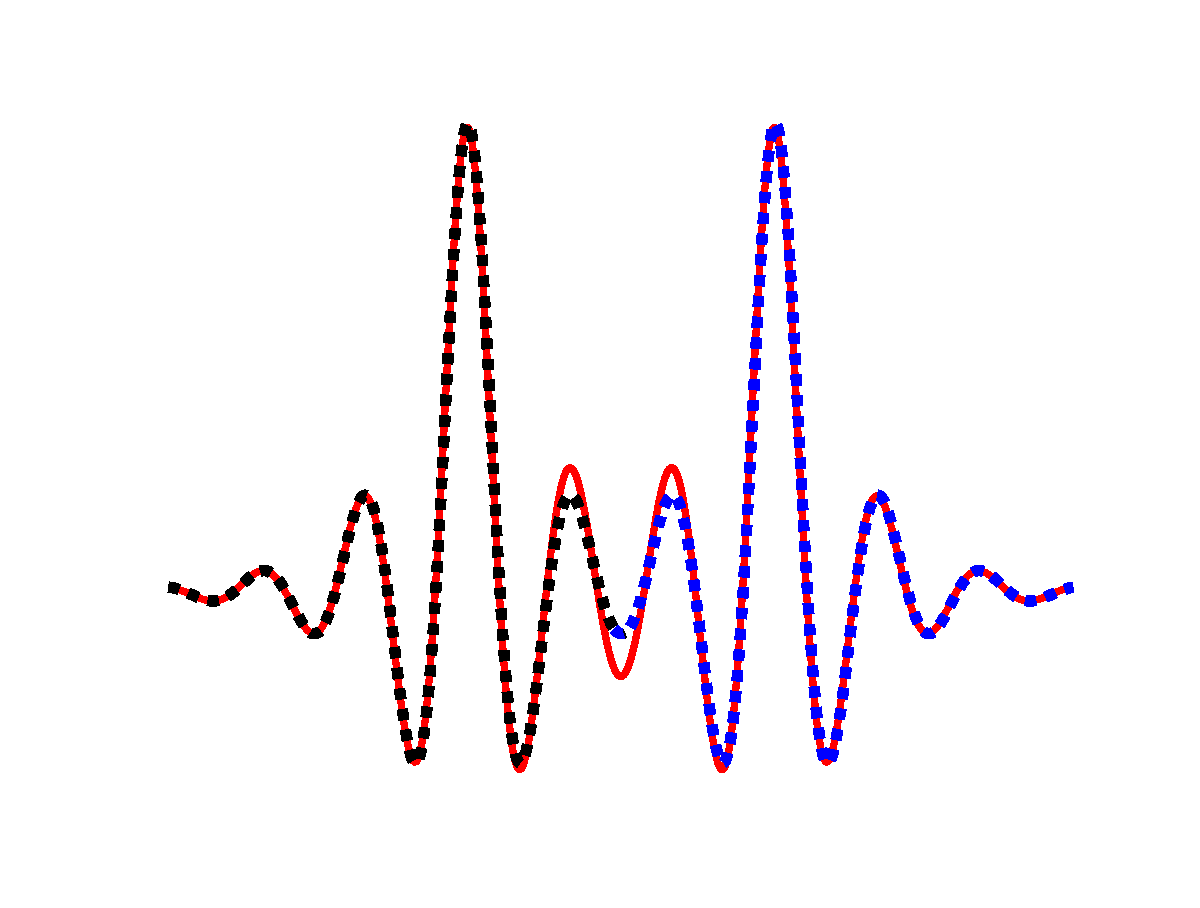
\includegraphics[width=7cm]{images/dpconstruction.eps} &
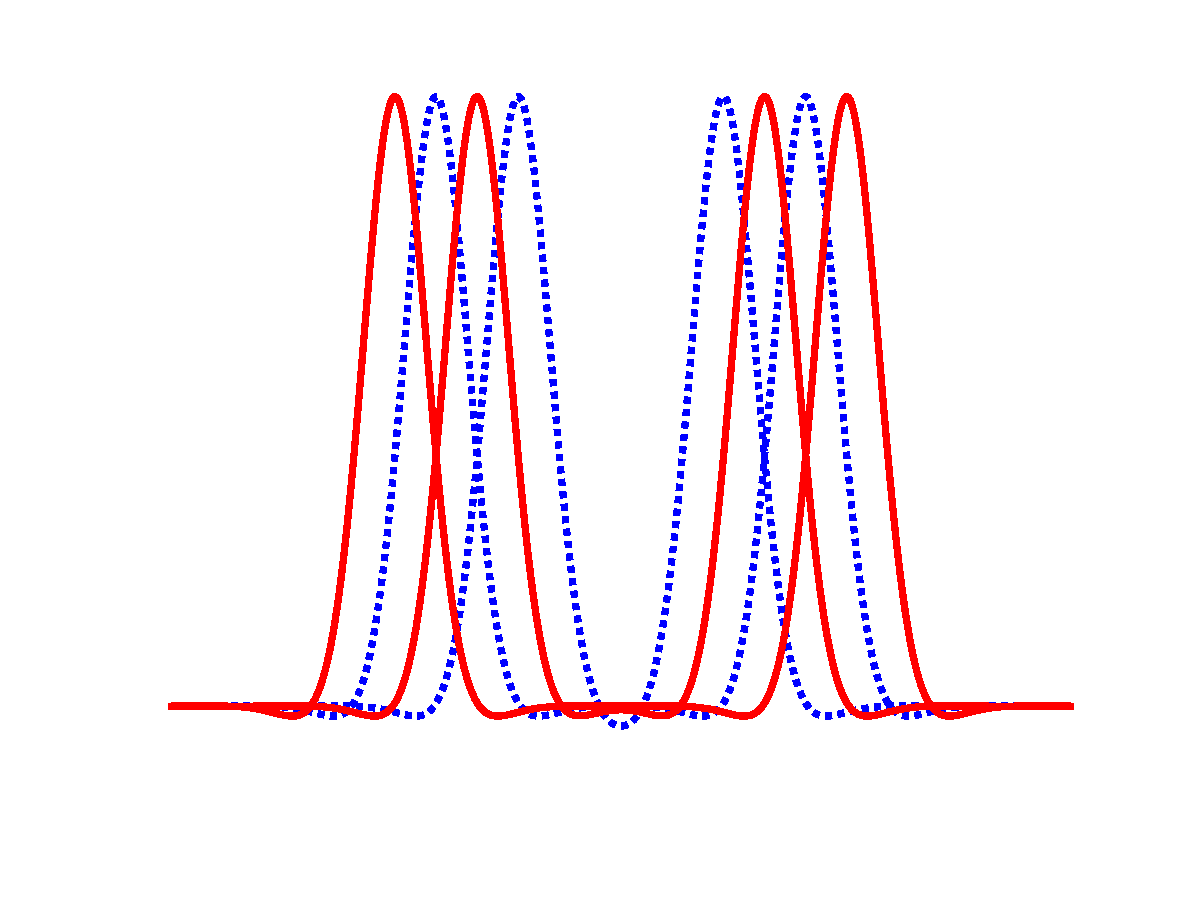
\includegraphics[width=7cm]{images/doublepulsealt.eps}
\end{tabular}
\end{center}
\caption{Left panel shows construction of double pulse solution (solid line) from two single pulses (dotted lines). Oscillatory tails are exaggerated. Right panel shows first four double pulse solutions.}
\label{fig:KdV5double}
\end{figure} 
\noi For the spectral problem, the essential spectrum is the entire imaginary axis, and depends only on the background state. 
% In addition, there is a set of interaction eigenvalues, which must occur in one of the three patterns in \cref{fig:kdv5inteigpattern} since equation \cref{KdV5example} is Hamiltonian. 
% \begin{figure}[H]
% \begin{center}
% 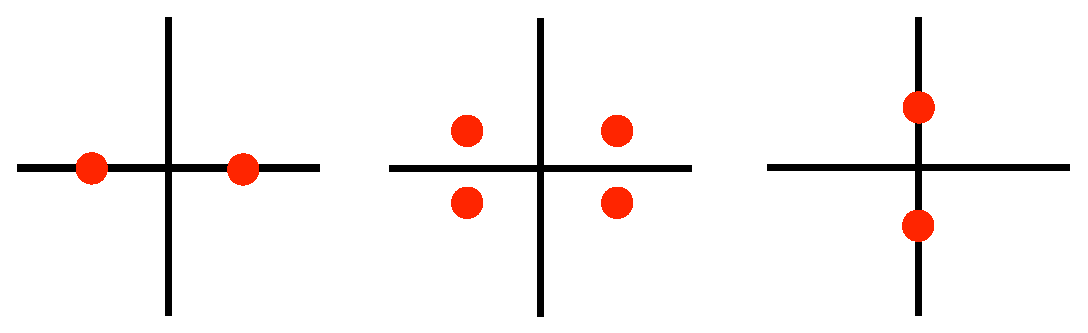
\includegraphics[width=8cm]{images/KdV5eigpattern}
% \end{center}
% \caption{Possible interaction eigenvalue patterns for double pulse solutions to KdV5.}
% \label{fig:kdv5inteigpattern}
% \end{figure}
\noi In addition, there is a pair of interaction eigenvalues which is symmetric about the origin and alternates between real (corresponding to double pulses with dashed lines in \cref{fig:KdV5double}, right panel) and imaginary with negative Krein signature (corresponding to double pulses with solid lines in \cref{fig:KdV5double}, right panel) \cite{Pelinovsky2007}. Numerical timestepping verifies that double pulses with real eigenvalues are unstable; when perturbed, the two peaks move away from each other with equal and opposite velocities (\cref{fig:KdV5waterfall}, left panel). For the remaining double pulses, numerical timestepping suggests that the two peaks exhibit oscillatory behavior when perturbed (\cref{fig:KdV5waterfall}, right panel). Similar timestepping results can be seen in \cite[Figure 9]{Pelinovsky2007}, as well as a reduction of the system to a two-dimensional phase plane \cite[Figure 10]{Pelinovsky2007}.

\begin{figure}[H]
\begin{center}
\begin{tabular}{cc}

\includegraphics[width=8cm]{images/waterfallunstable.eps} &
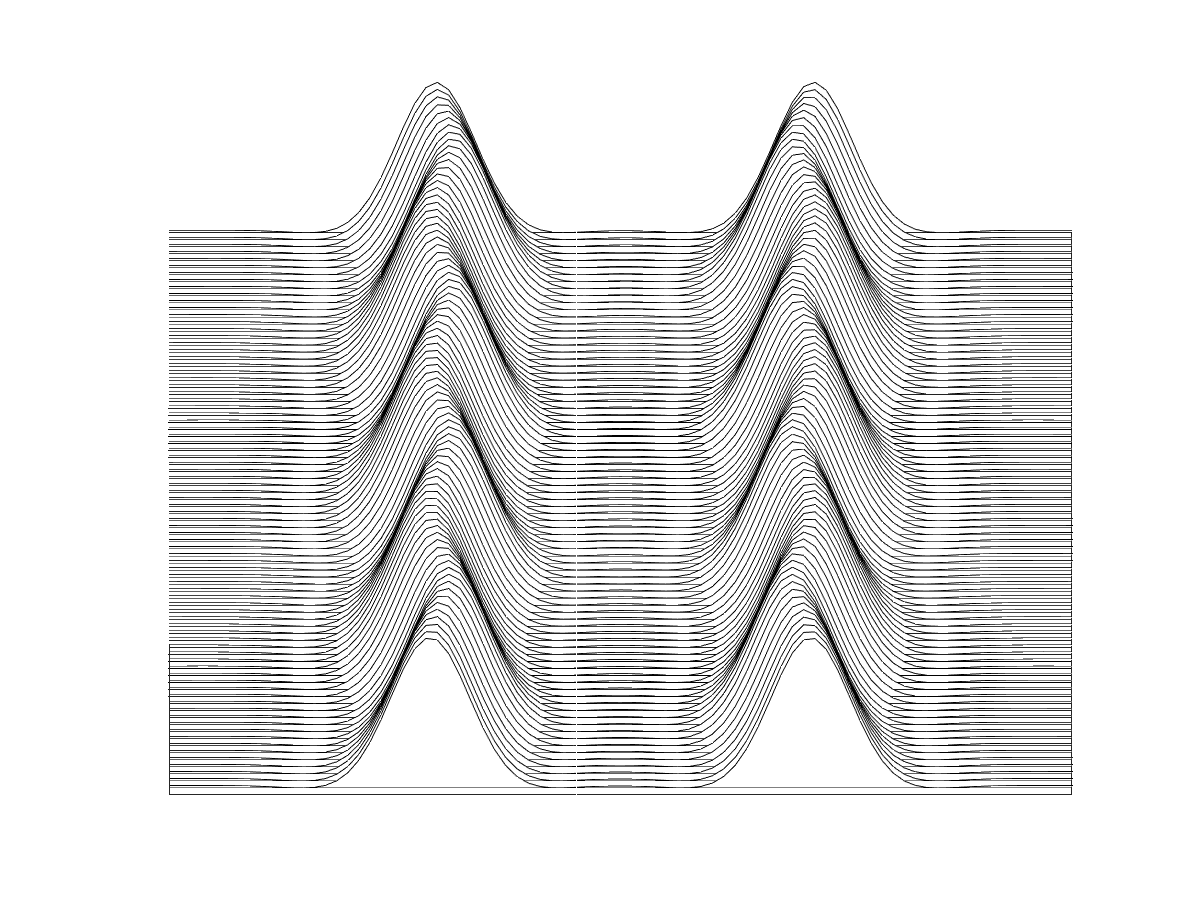
\includegraphics[width=8cm]{images/waterfallstable.eps}
\end{tabular}
\end{center}
\caption{Results of numerical timestepping simulations for perturbations of double pulse solutions to \cref{KdV5example}. Crank-Nicolson/Adams-Bashforth 2 IMEX scheme in time with Chebyshev spectral discretization, Dirichlet and Neumann boundary conditions.}
\label{fig:KdV5waterfall}
\end{figure}

% \noi This suggests that the dynamics of perturbed double pulses can be reduced to a 2-dimensional system, where the variables are the peak distance and peak relative velocity (\cref{fig:KdV5reduction}). The phase portrait resembles that of a harmonic oscillator with spatially varying restoring force. Double pulses with real eigenvalues correspond to saddle points, and the remaining double pulses correspond to centers. 
% \begin{figure}[H]
% \begin{center}
% \begin{tabular}{c}
% 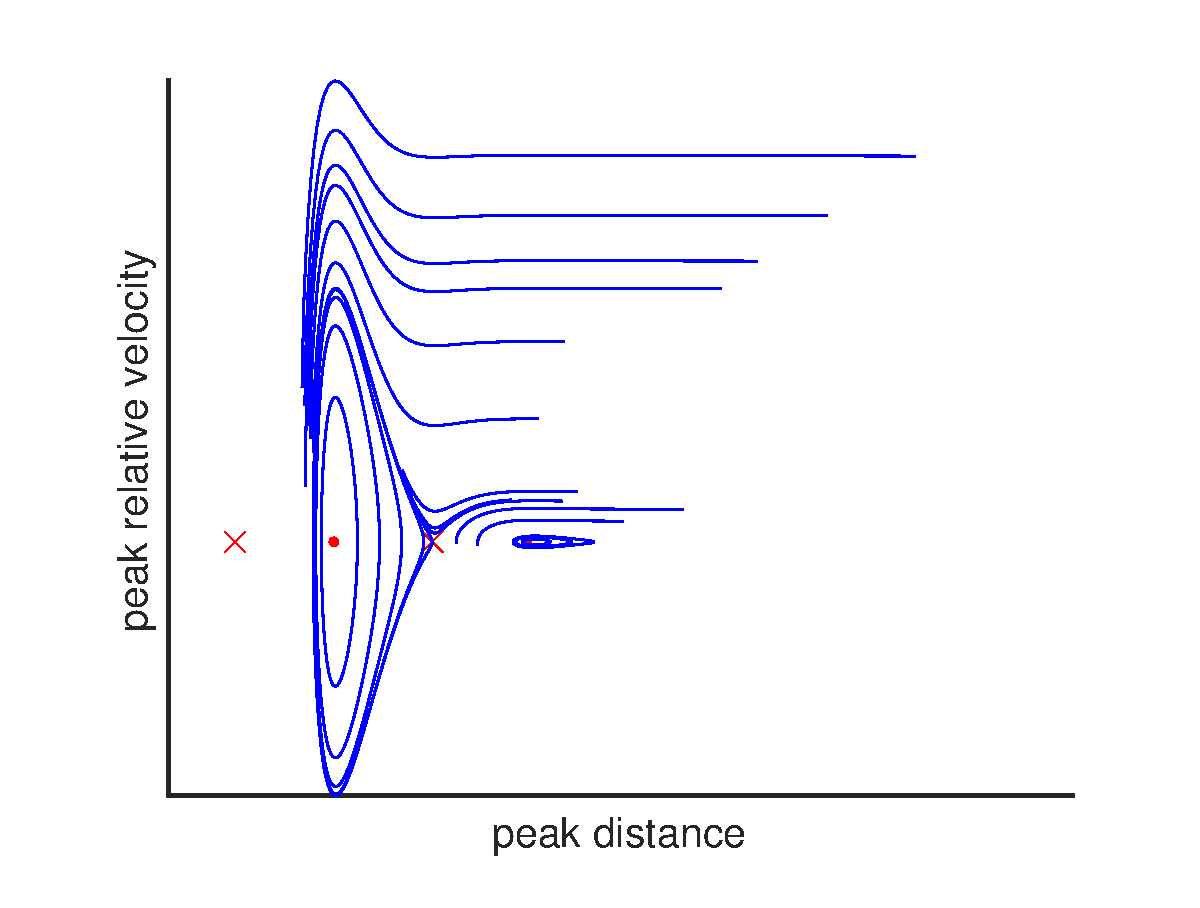
\includegraphics[width=7cm]{images/reduction.eps}
% \end{tabular}
% \end{center}
% \caption{Plot of peak relative velocity versus peak distance for perturbed double pulses.}
% \label{fig:KdV5reduction}
% \end{figure}

\noi Although these numerical results suggest that every other double pulse is neutrally stable, this remains an open question since the imaginary eigenvalues are embedded in the essential spectrum. Furthermore, the timestepping simulation was performed with separated boundary conditions, which shifts the essential spectrum into the left half plane and thus could fundamentally alter the behavior of the system.

As an alternative, we look at multi-pulse solutions on a periodic domain. Periodic traveling waves were described by Korteweg and de Vries in their 1895 paper \cite{KdVoriginal}, and the stability of these cnoidal waves is shown in \cite{Pava2006,Bottman2009}. Since then, stability of periodic solutions has been investigated for many other systems, including the generalized KdV equation \cite{Johnson2009}, the generalized Kuramoto-Sivashinsky equation \cite{Barker2013}, the Boussinesq equation \cite{Hakkaev2014}, the Klein-Gordon equation \cite{Demirkaya2015}, a generalized class of nonlinear dispersive equations \cite{Hur2015}, and the regularized short pulse and Ostrovsky equations \cite{Hakkaev2017}. In this paper, we consider multi-pulse solutions on a periodic domain $[-X, X]$ subject to co-periodic perturbations. The essential spectrum becomes a discrete set of points on the imaginary axis, and purely imaginary interaction eigenvalues can lie within gaps in the essential spectrum. As long as the interaction eigenvalues and the essential spectrum do not get too close, we show that the interaction eigenvalues for double pulses on a periodic domain are either real or purely imaginary. As the domain size $X$ is increased, however, the essential spectrum eigenvalues move along the imaginary axis towards the origin. At a critical value of $X$, there can be a collision between one of these essential spectrum eigenvalues and a purely imaginary interaction eigenvalue. Since the two eigenvalues have opposite Krein signature, we expect them to leave the imaginary axis upon collision. In fact, what occurs is that a brief instability bubble is formed, where the two eigenvalues collide, move off the imaginary axis, trace an approximate circle in the complex plane, and recombine on the imaginary axis in a ``reverse'' Krein collision. This brief instability bubble, which we call a Krein bubble, is shown in cartoon form in \cref{fig:KreinBubbleCartoon}.
\begin{figure}[H]
\begin{center}
\begin{tabular}{c}
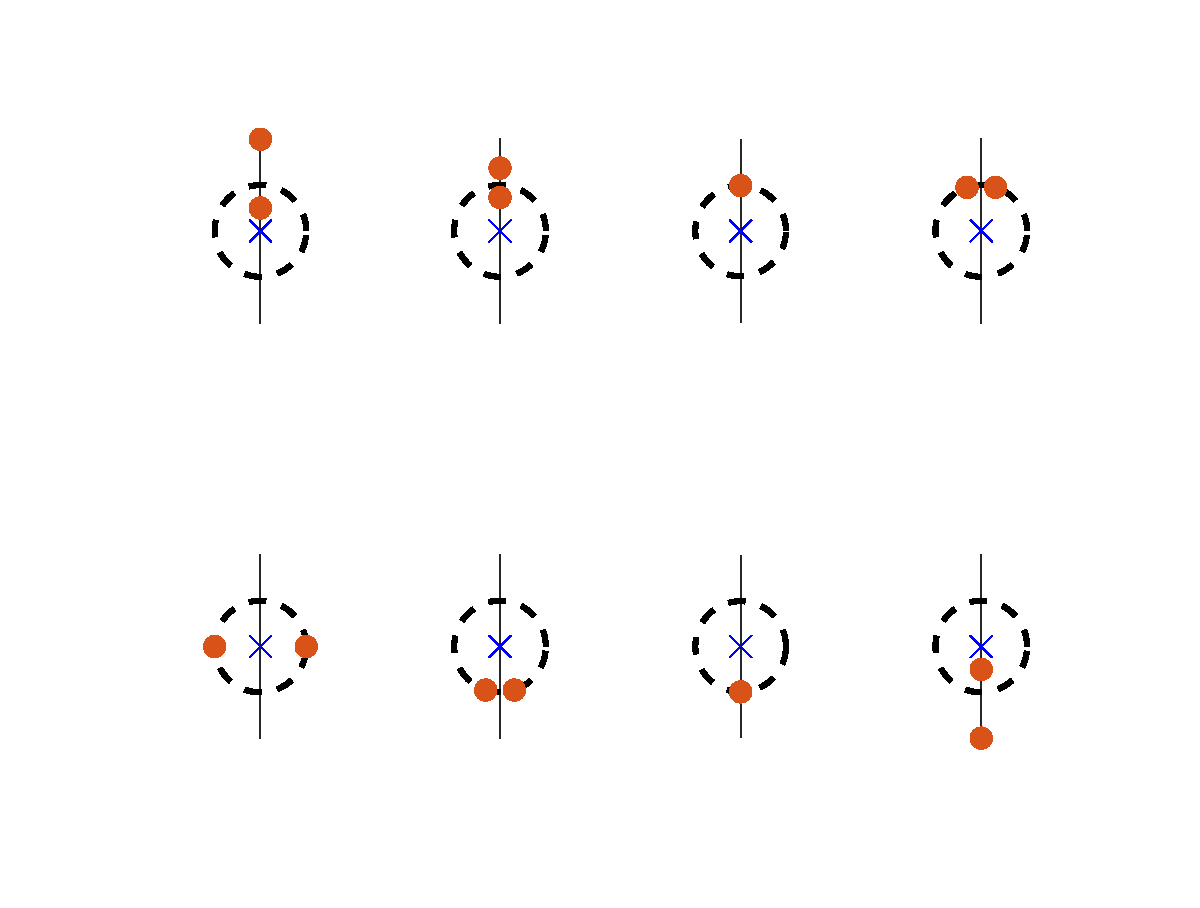
\includegraphics[width=15cm]{images/KreinBubbleCartoon.eps}
\end{tabular}
\end{center}
\caption{Cartoon showing brief instability bubble which forms as imaginary interaction eigenvalue and first essential spectrum eigenvalue collide on imaginary axis. Eigenvalues are shown in red dots, center of instability bubble is marked with blue X.}
\label{fig:KreinBubbleCartoon}
\end{figure}
\noi Similar instability bubbles have been observed in other systems. As one example, they are found for dark soliton solutions of the discrete nonlinear Schr{\"o}dinger equation on a finite lattice as the coupling parameter is increased \cite{Johansson1999}; in that case, however, the instability bubbles disappear after a critical value of the coupling parameter is reached (\cite[Figure 2]{Johansson1999}).

This paper is organized as follows. In \cref{sec:KdV5}, we introduce a generalization of KdV5 as our motivating example. In \cref{sec:setup}, we set up the problem of interest in general terms as a Hamiltonian system which is reversible and translation invariant, for which KdV5 is a special case. We then present the main results of this paper, which concern the existence (\cref{sec:perexist}) and spectrum (\cref{sec:perstab}) of periodic multi-pulse solutions. This is then applied to the periodic single pulse and the periodic double pulse. In particular, we prove that Krein bubbles occur and give a formula for their radius in terms of fundamental constants associated with the system. In \cref{sec:numerics}, we present numerical results which provide verification for our theoretical work. The next sections contain proofs of the main results, after which we discuss our findings in \cref{sec:conclusions} and offer some directions for future work. 

\section{Background and motivation}\label{sec:KdV5}

The Kawahara equation, also known as a fifth-order KdV-type equation, is used as a model for water waves, magneto-acoustic waves, plasma waves, and other dispersive phenomena. This equation takes the general form
\begin{equation}\label{kawahara}
u_t + \alpha u_{xxx} + \beta u_{xxxxx} = \frac{\partial}{\partial x} f(u, u_x, u_{xxx}),
\end{equation}
where $u(x, t)$ is a real-valued function, the parameters $\alpha$ and $\beta$ are real with $\beta \neq 0$, and $f$ is a smooth function \cite{Bridges2002,Bridges2002a}. If $f$ is a variational derivative, then \cref{kawahara} is the Hamiltonian system $\partial_t u = \calJ \calE'(u)$, where $\calJ = \partial_x$ is skew-Hermitian,
\begin{equation}\label{kawaharaE}
\calE(u) = -\frac{1}{2}\int_{-\infty}^\infty 
\left( \frac{1}{2}u_{xx}^2 - \frac{1}{2}\alpha u_x^2 + h(u, u_x, u_{xx})\right)dx
\end{equation}
is the energy, and $f$ in \cref{kawahara} is the variational derivative of the term involving $h$ in \cref{kawaharaE} \cite{Bridges2002}. A prototypical example is
\[
u_t + \frac{2}{15}u_{xxxxx} - b u_{xxx} + 3 u u_x + 2 u_x u_{xx} + u u_{xxx} = 0,
\]
which is a weakly nonlinear long-wave approximation for capillary-gravity water waves \cite{Champneys1998,Champneys1997}. We will consider instead the simpler equation 
\begin{equation}\label{KdV5}
u_t = u_{xxxxx} + p u_{xxx} - 2 u u_x,
\end{equation}
which is a general form of \cite[(1)]{Pelinovsky2007}. Writing \cref{KdV5} in a co-moving frame with speed $c$ by letting $\xi = x - ct$, equation \cref{KdV5} becomes
\begin{equation}\label{KdV5c}
u_t = \partial_x(u_{xxxx} + p u_{xx} + cu - u^2),
\end{equation}
where we have renamed the independent variable back to $x$. Localized traveling pulse solutions satisfy the 4th order ODE
\begin{equation}\label{KdV5eq4}
u_{xxxx} + p u_{xx} + c u - u^2 = 0,
\end{equation}
which is obtained from \cref{KdV5c} by integrating once. Equation \cref{KdV5eq4} is Hamiltonian, with conserved quantity
\begin{equation}\label{KdV5ham}
H(u, u_x, u_{xx}, u_{xxx}) = u_x u_{xxx} - \frac{1}{2}u_{xx}^2 + \frac{p}{2}u_x^2 + \frac{c}{2}u^2 - \frac{1}{3}u^3,
\end{equation}
which is obtained by multiplying \cref{KdV5eq4} by $u_x$ and integrating once. Letting
\begin{equation}\label{KdV5U}
U = (q_1, q_2, p_1, p_2) = (u, u_x, -u_{xxx} + u_x, u_{xx}),
\end{equation}
we can also write \cref{KdV5eq4} in standard Hamiltonian form as the first order system
\begin{equation}\label{KdV5ham2}
U' = F(U) = J \nabla \tilde{H}(U),
\end{equation}
where $J$ is the standard $4 \times 4$ symplectic matrix and
\begin{equation}
\tilde{H}(q_1, q_2, p_1, p_2) = \frac{1}{3}q_1^3 - \frac{1}{2}c q_1^2 + p_1 q_2 + \frac{p}{2}q_2^2 + \frac{1}{2}p_2^2.
\end{equation}
We have the following theorem concerning the existence of localized solutions to \cref{KdV5eq4}, which is a direct consequence of \cite{Groves1998}, reversibility, and the stable manifold theorem.

\begin{theorem}\label{KdV1pulse}
If $p < 2 \sqrt{c}$, then there exists a one-pulse solution $q(x)$ to \cref{KdV5eq4} which is an even function and decays exponentially to 0 at $\pm \infty$.
\end{theorem}

Linearization of \cref{KdV5eq4} about a solution $u^*(x)$ is the self-adjoint linear operator
\begin{equation}\label{KdV5hessian}
\calE''(u^*) = \partial_x^4 + p \partial_x^2 + c - 2 u^*,
\end{equation}
where $\calE''(u^*)$ is the Hessian of the energy. The rest state $u = 0$ corresponds to the equilibrium point $U = 0$ of the first order system \cref{KdV5ham2}. When $p < 2 \sqrt{c}$, this equilibrium is a hyperbolic saddle with 2-dimensional stable and unstable manifolds. The primary pulse $q(x)$ corresponds to a homoclinic orbit connecting the stable and unstable manifolds of this equilibrium. If $-2 \sqrt{c} < p < 2 \sqrt{c}$, the eigenvalues of $DF(0)$ are a complex quartet $\pm \alpha_0 \pm \beta i_0$, and multi-modal homoclinic and periodic orbits exist which lie close to the primary homoclinic orbit. We adapt Lin's method as in \cite{Sandstede1993, SandstedeStrut} to construct periodic multi-pulse solutions by gluing together consecutive copies of the primary pulse in a loop using small remainder functions. This provides not only an existence result but also estimates for these small remainder functions. As opposed to $n$-homoclinic solutions, which require $n-1$ joins at the pulse tails, these $n$-periodic solutions require $n$ joins at the tails, which provides an additional degree of freedom. For periodic double pulses, this leads to a pitchfork bifurcation structure, whereby solutions with unequal pulse distances bifurcate from those with equal pulse distances. For spectral stability, as in \cite{Sandstede1998}, we reduce the computation of the spectrum of the linearization of the PDE \eqref{KdV5c} about a periodic $n$-pulse to a matrix equation. In contrast to \cite{Sandstede1998}, we obtain a $2n \times 2n$ block matrix which encodes both the interaction eigenvalues and the essential spectrum eigenvalues near the origin.


\section{Mathematical Setup}\label{sec:setup}

\subsection{Hamiltonian PDE}\label{sec:HamPDE}

First, we define a Hamiltonian PDE which is reversible and translation invariant. This analysis follows Grillakis, Shatah, and Strauss \cite{Grillakis1987}. Let $X = H^{2m}(\R)$ and $Y = L^2(\R)$, and consider the PDE
\begin{equation}\label{genPDE}
u_t = \partial_x \calE'(u),
\end{equation}
where $u \in X$ and $\calE: X \subset Y \rightarrow \R$ is a smooth functional representing the conserved energy of the system. We take the following hypothesis regarding the energy $\calE(u)$.

\begin{hypothesis}\label{hyp:E}
The energy $\calE(u)$ has the following properties:
\begin{enumerate}[(i)]
\item $\calE(0) = 0$ and $\calE'(0) = 0$.
\item $\calE(u) = \calE(\rho(u))$, where $\rho: X \rightarrow X$ is the reversor operator $[\rho(u)](x) = u(-x)$.
\item $\calE(T(s)u) = \calE(u)$ for all $s \in \R$, where $\{T(s) : s \in \R \}$ is the one parameter group of unitary translation operators on $X$ defined by $[T(s)]u(\cdot) = u(\cdot - s)$.
\item $\calE'(u): X \rightarrow X$ is a differential operator of the form
\begin{equation}\label{Eprimeuform}
\calE'(u) = \partial_x^{2m}u - f(u, \partial_x u, \dots, \partial_x^{2m-1} u),
\end{equation}
where $f: \R^{2m} \rightarrow \R$ is smooth.
\end{enumerate}
\end{hypothesis}

\noi \cref{hyp:E}(ii) is reversibility, and \cref{hyp:E}(iii) is translation invariance. \cref{hyp:E}(iv) holds in applications such as KdV5, and lets us write the $2m$-th order ODE $\calE'(u) = 0$ as a first order system in $\R^{2m}$. Differentiating the reversibility relation $\calE(u) = \calE(\rho(u))$ with respect to $u$,
\[
\calE'(u) = \rho^*( \calE'(\rho(u) ) = \rho( \calE'(\rho(u) ),
\]
since $\rho$ is self-adjoint. Differentiating the symmetry relation $\calE(T(s)u) = \calE(u)$ with respect to $u$,
\begin{align}
\calE'(u) &= T(s)^* \calE'(T(s)u) \label{Eprimesymm} \\
\calE''(u) &= T(s)^* \calE''(T(s)u) T(s). \label{EHessiansymm}
\end{align}
Differentiating the symmetry relation $\calE(T(s)u) = \calE(u)$ with respect to $s$ at $s = 0$, 
\begin{align*}
0 = \langle \calE'(u), T'(s) u \rangle|_{s = 0}
= \langle \calE'(u), T'(0) u \rangle
= \langle \calE'(u), \partial_x u \rangle
\end{align*}
for all $u \in X$, since $T'(0) = \partial_x$ is the infinitesimal generator of the translation group $T(s)$. There is an additional conserved quantity $\calQ: L^2(\R) \rightarrow \R$, given by
\begin{equation}\label{defV}
\calQ(u) = -\frac{1}{2} \int_{-\infty}^\infty u^2 dx,
\end{equation}
which represents charge in some applications. Traveling waves are solutions of \cref{genPDE} of the form $u(x, t) = T(ct)\phi(x) = \phi(x - ct)$. If $\phi$ satisfies the equilibrium equation $\calE'(\phi) = c \calQ'(\phi)$, then $T(ct)\phi(x)$ is a traveling wave \cite{Grillakis1987}. Since $\calQ'(\phi) = -\phi$, the equilibrium equation becomes
\begin{equation}\label{eqODE}
\calE'(\phi) + c \phi = 0.
\end{equation}
Without loss of generality, we will assume that $\calE'(\phi)$ does not contain any terms of the form $b\phi$ for $b$ constant, since that is accounted for by the $c \phi$ term in \cref{eqODE}.

We take the following hypothesis concerning existence of traveling waves, which is similar to \cite[Assumption 2]{Grillakis1987}. In the next section, we will give a condition under which this hypothesis is satisfied. 
\begin{hypothesis}\label{hyp:cinterval}
There exists an open interval $(c_1, c_2) \subset \R$ and a $C^1$ map $c \mapsto \phi_c$ such that for every $c \in (c_1, c_2)$, $\calE'(\phi_c) + c \phi_c = 0$, i.e. $\phi_c$ is a traveling wave solution to \cref{genPDE}.
\end{hypothesis}

The linearization of the PDE \cref{genPDE} about a traveling wave solution $\phi_c$ is the linear operator $\partial_x \calL(\phi_c)$, where $\calL(\phi_c)$ is the self-adjoint operator
\begin{equation}\label{PDElinearization}
\calL(\phi_c) = \calE''(\phi_c) + c,
\end{equation}
and $\calE''(\phi_c)$ is the Hessian of the energy $\calE(\phi_c)$. Differentiating \cref{eqODE} with respect to $x$ and with respect to $c$,
\begin{equation}\label{Lkernel}
\begin{aligned}
\calL(\phi_c) \partial_x \phi_c &= 0 \\
\calL(\phi_c) (-\partial_c \phi_c)& = \phi_c.
\end{aligned}
\end{equation}
Differentiating again with respect to $x$,
\begin{equation}\label{Ekernel}
\begin{aligned}
[\partial_x \calL(\phi_c)] \partial_x \phi_c &= 0 \\
[\partial_x \calL(\phi_c)](-\partial_c \phi_c) &= \partial_x \phi_c,
\end{aligned}
\end{equation}
thus the kernel of $\partial_x \calE''(\phi_c)$ has algebraic multiplicity at least 2 and geometric multiplicity at least 1.

\subsection{Spatial dynamics formulation}\label{sec:spatdym}

We reformulate the equilibrium equation \cref{eqODE} using a spatial dynamics approach by rewriting it as a first-order dynamical system in $\R^{2m}$ evolving in the spatial variable $x$. From this viewpoint, an exponentially localized traveling wave is a homoclinic orbit connecting a saddle point equilibrium to itself. Let $U = (u, \partial_x u, \dots, \partial_x^{2m-1} u)^T \in \R^{2m}$. Using \cref{hyp:E}(iv), equation \cref{eqODE} is equivalent to the first order system
\begin{equation}\label{genODE}
U'(x) = F(U(x); c),
\end{equation}
where $F: \R^{2m} \times \R \rightarrow \R^{2m}$ is smooth and is given by
\begin{equation}\label{defF}
F(u_1, u_2, \dots, u_{2m}; c) = 
\begin{pmatrix}
u_2 \\ u_3 \\ \vdots \\ f(u_1, u_2, \dots, u_{2m}) - c u_1
\end{pmatrix}.
\end{equation}
By reversibility,
\begin{equation}\label{genODErev}
\begin{aligned}
F(RU; c) &= -RF(U; c) \\
DF(RU; c) &= -RDF(U; c)R,
\end{aligned}
\end{equation}
where $R:\R^{2m} \rightarrow \R^{2m}$ is the standard reversor operator on $\R^{2m}$
\begin{equation}\label{reverserR2m}
R(u_1, u_2, \dots, u_{2m-1}, u_{2m}) = (u_1, -u_2, \dots, u_{2m-1}, -u_{2m}).
\end{equation}
First, we assume that \cref{genODE} is a conservative system.
\begin{hypothesis}\label{hyp:H}
There exists a smooth function $H: \R^{2m} \times \R \rightarrow \R$ such that 
\begin{enumerate}[(i)]
\item $H(0; c) = 0$ for all $c$.
\item $\nabla_U H(U; c) = 0$ if and only if $F(U; c) = 0$.
\item For all $U \in \R^{2m}$ and all $c$, $\langle F(U; c), \nabla_U H(U; c) \rangle = 0$.
\end{enumerate}
\end{hypothesis}

\noi It follows from \cref{hyp:H} that $H$ is conserved along solutions to \cref{genODE}. Since $F(0; c) = 0$ for all $c$, the rest state $U = 0$ is an equilibrium of \cref{genODE} for all $c$. The next hypothesis addresses the hyperbolicity of this equilibrium. Although the eigenvalue pattern described in \cref{hyp:hypeq} is not necessary for the existence of a homoclinic orbit solution, it is a sufficient condition for the existence of multi-pulse and periodic multi-pulse solutions.

\begin{hypothesis}\label{hyp:hypeq}
For a specific $c_0 > 0$, $U = 0$ is a hyperbolic equilibrium of \cref{genODE}. Furthermore, the spectrum of $DF(0; c_0)$ contains a quartet of simple eigenvalues $\pm \alpha_0 \pm \beta_0 i$, $\alpha_0, \beta_0 > 0$, and for any other eigenvalue $\nu$ of $DF(0; c_0)$, $|\text{Re }\nu| > \alpha_0$.
\end{hypothesis}

We now address the existence of a primary pulse solution, which is a symmetric homoclinic orbit connecting the unstable manifold $\tilde{W}^u(0; c_0)$ and the stable manifold $\tilde{W}^s(0; c_0)$ of the rest state equilibrium. Both of these manifolds have dimension $m$ by reversibility. Since, in general, the existence of such a solution is unknown, we take the existence of a primary pulse solution for a specific wavespeed $c_0$ as a hypothesis.

\begin{hypothesis}\label{Qexistshyp}
For the same $c_0$ as in \cref{hyp:hypeq}, there exists a homoclinic orbit solution $Q_1(x; c_0) = (q(x; c_0), \partial_x q(x; c_0), \dots, \partial_x^{2m-1}q(x; c_0))^T\in \tilde{W}^s(0) \cap \tilde{W}^u(0) \subset H^{-1}(0; c_0)$ to \cref{genODE}. In addition,
\begin{enumerate}[(i)]
\item $Q_1(0; c_0) \neq 0$.
\item $\nabla_U H(Q_1(0; c_0); c_0) \neq 0$.
\item $Q_1(x; c_0)$ is symmetric with respect to the reversor operator \cref{reverserR2m}, i.e. $Q_1(-x; c_0) = R Q_1(x; c_0)$.
\end{enumerate}
\end{hypothesis}

\noi It follows from \cref{Qexistshyp} that $q(x; c_0)$ is a symmetric, exponentially localized traveling wave solution solution to \cref{genPDE}. In order to prove the  existence of homoclinic orbits $Q_1(x; c)$ for $c$ near $c_0$, we take the following additional hypothesis.

\begin{hypothesis}\label{hyp:transverse}
The stable manifold $\tilde{W}^s(0; c_0)$ and the unstable manifold $\tilde{W}^u(0; c_0)$ intersect transversely in $H^{-1}(0; c_0)$ at $Q_1(0; c_0)$.
\end{hypothesis}

\noi Using \cref{hyp:transverse} and a dimension-counting argument, we obtain the nondegeneracy condition
\begin{equation}\label{nondegencond}
T_{Q_1(0; c_0)}W^s(0; c_0) \cap T_{Q_1(0; c_0)}W^u(0; c_0) = \R Q_1'(0; c_0).
\end{equation}
We then have the following existence theorem. The proof is given in \cref{sec:transverseintproof}.

\begin{theorem}\label{transverseint}
Assume \cref{hyp:H} and \cref{hyp:transverse}. Then there exists $\delta_0 > 0$ such that for $c \in (c_0 - \delta_0, c_0 + \delta_0)$, the stable and unstable manifolds $\tilde{W}^s(0; c)$ and $\tilde{W}^u(0; c)$ have a one-dimensional transverse intersection in $H^{-1}(0; c)$ which is a homoclinic orbit $Q_1(x; c)$. $Q_1(-x; c) = R Q_1(x; c)$, the map $c \rightarrow Q_1(x; c)$ is smooth, and $\partial_c Q_1(x; c)$ is exponentially localized, i.e. for any $\epsilon > 0$ there exists $\delta_1 > 0$ with $\delta_1 \leq \delta_0$ such that for $c \in (c_0 - \delta_1, c_0 + \delta_1)$,
\begin{equation}\label{Qcbound}
|\partial_c Q_1(x; c)| \leq C e^{-(\alpha_0 - \epsilon)|x|}.
\end{equation}
\end{theorem}

Finally, as in \cite{Grillakis1987}, define the scalar $d(c) = \calE(q(x, c)) - \omega\calQ(q(x, c))$. By \cite{Bona1987,Grillakis1987}, the traveling wave $q(x, c)$ is orbitally stable if $d''(c) > 0$, where
\begin{align}\label{ddoubleprime}
d''(c) = \langle \calQ'(q(x, c)), \partial_c q(x, c) \rangle
= \int_{-\infty}^\infty q(x, c) \partial_c q(x, c) dx.
\end{align}
This can be computed numerically, and we take this stability criterion as a hypothesis.

\begin{hypothesis}\label{hyp:dccpos}
For each $c \in (c_0 - \delta_0, c_0 + \delta_0)$, where $\delta_0$ is defined in \cref{transverseint}, $d''(c) > 0$.
\end{hypothesis}

\noi From this point on, we will fix a speed $c \in (c_0 - \delta_0, c_0 + \delta_0)$ and suppress the dependence on $c$ for notational simplicity.

\subsection{Eigenvalue problem}\label{sec:EVP}

Let $U^*(x) = (u^*(x), \partial_x u^*(x), \dots, \partial_x^{2m-1}u^*(x) )^T$ be any solution to \cref{genODE}, so that $u^*(x)$ is a traveling wave solution to \cref{genPDE}.
Then $u^*(x)$ solves the equation $\partial_x(\calE'(u) + cu) = 0$, which is equivalent to the system
\begin{equation}\label{eqsystem2}
\begin{aligned}
\calE'(u) + cu &= k \\
\partial_x k &= 0.
\end{aligned}
\end{equation}
Using a spatial dynamics approach, we rewrite \cref{eqsystem2} as
\begin{equation}\label{spsystem2}
\begin{pmatrix}
U \\ k
\end{pmatrix}'(x) =
\begin{pmatrix} 
F(U(x)) + k e_{2m} \\ 0
\end{pmatrix},
\end{equation}
where $e_{2m} = (0, \dots, 0, 1)^T \in \R^{2m}$ is the standard unit vector. We similarly reformulate the PDE eigenvalue problem $\partial_x \calL(u^*) v = \lambda v$ as the system 
\begin{equation}\label{genPDEeig2}
\begin{aligned}
\calL(u^*) v &= k \\
\partial_x k &= \lambda v,
\end{aligned}
\end{equation}
which is equivalent to the first order system in $\C^{2m+1}$
\begin{equation}\label{PDEeigsystem}
V'(x) = A(U^*(x))V(x) + \lambda B V(x),
\end{equation}
where $A(U^*(x))$ and $B$ are the $(2m+1) \times (2m+1)$ matrices
\begin{equation}\label{defAB}
A(U^*(x)) = 
\begin{pmatrix}
DF(U^*(x)) & e_{2m}\\
0 & 0
\end{pmatrix}, \qquad
B = \begin{pmatrix}0 & 0 & \cdots & 0 \\ & 
\vdots & \vdots & \\0 & 0 & \cdots & 0 \\ 1 & 0 & \cdots & 0 \end{pmatrix}.
\end{equation}
$A(0)$ has a one-dimensional kernel, which is characterized in the following lemma. 

\begin{lemma}\label{eigA0lemma}
The matrix $A(0)$ has a simple eigenvalue at 0 and a quartet of eigenvalues $\pm \alpha_0 \pm \beta_0 i$. For any other eigenvalue $\nu$ of $A(0)$, $|\text{Re }\nu| > \alpha_0$. The kernel of $A(0)$ is spanned by $V_0$ and the kernel of $A^*(0)$ is spanned by $W_0$, where
\begin{equation}\label{V0W0}
V_0 = \left(\frac{1}{c}, 0, \dots, 0, 1\right)^T, \quad
W_0 = (0, 0, \dots, 0, 1)^T,
\end{equation}
and $\langle V_0, W_0 \rangle = 1$. The projection on $\R V_0$ is given by $P_{V_0} = \langle W_0, \cdot \rangle$.
\begin{proof}
Let $p_1(\nu)$ and $p_2(\nu)$ be the characteristic polynomials of $DF(0)$ and $A(0)$. Since
\begin{align*}
p_2(\nu) &= \det(A(0) - \nu I) = -\nu \det(DF(0) - \nu I) = -\nu p_1(\nu),
\end{align*}
$A(0)$ has the same eigenvalues as $DF(0)$ as well as an additional eigenvalue at 0, thus part (i) follows from \cref{hyp:hypeq}. The kernel eigenvectors $V_0$ and $W_0$ and the projection $P_{V_0}$ can be verified directly.
\end{proof}
\end{lemma}

Since $A(0)$ is non-hyperbolic, the rest state $(U, k) = (0, 0)$ is a non-hyperbolic equilibrium of \cref{spsystem2}, and the results of \cite{Sandstede1998} do not apply. Let $W^s(0)$, $W^u(0)$, and $W^c(0)$ be the stable, unstable, and center manifolds of the equilibrium at the origin. By reversibility, $\dim W^s(0) = m$ and $\dim W^u(0) = m$, and $\dim W^c(0) = 1$. Let $Q_1(x)$ be the primary pulse solution from \cref{transverseint}, and let $Q(x) = (Q_1(x), 0)$. The associated variational and adjoint variational equations are
\begin{align}
V'(x) &= A(Q(x)) V(x) \label{vareq2} \\
W'(x) &= -A(Q(x))^* W(x) \label{adjvareq2},
\end{align}
and $Q'(x)$ is an exponentially localized solution to \cref{vareq2}. Since $Q(x)$ is exponentially localized, $\R Q'(0) \subset T_{Q(0)}W^s(0) \cap T_{Q(0)}W^u(0)$. It follows from \cref{hyp:transverse} that these are in fact equal.

\begin{lemma}\label{nondegenlemma}
We have the nondegeneracy condition
\begin{equation}\label{nondegen2}
T_{Q(0)}W^s(0) \cap T_{Q(0)}W^u(0) = \R Q'(0).
\end{equation}
\begin{proof}
If the intersection were more than one-dimensional, there would exist another exponentially localized solution $V(x) = (v_1, \dots, v_{2m}, v_{2m+1})^T$ to \eqref{vareq2}. By the definition of $A(Q(x))$, $v_{2m+1}$ is a constant, which must be 0 since $V(x)$ is exponentially localized. Then $(v_1, \dots, v_{2m})^T$ would be an exponentially localized solution to $V'(x) = DF(Q(x)) V(x)$, which contradicts \eqref{nondegencond}.
\end{proof}
\end{lemma}

\noi Using \cref{nondegen2}, we can decompose the tangent spaces of the stable and unstable manifolds at $Q(0)$ as
\begin{equation}\label{TQ0decomp}
\begin{aligned}
T_{Q(0)}W^s(0) &= \R Q'(0) \oplus Y^+ \\
T_{Q(0)}W^u(0) &= \R Q'(0) \oplus Y^-.
\end{aligned}
\end{equation}
Since $\dim \R Q'(0) \oplus Y^+ \oplus Y^- = 2m-1$, we need two more directions to span $\R^{2m+1}$. We obtain these from the following lemma.

\begin{lemma}\label{varadjsolutions}
We have the following bounded solutions to the variational and adjoint variational equations.
\begin{enumerate}[(i)]
	\item There are two linearly independent, bounded solutions $Q'(x)$ and $V^c(x)$ to \eqref{vareq2}. $V^c(x) \rightarrow V_0$ as $|x| \rightarrow \infty$, and	$V^c(-x) = R V^c(x)$, where $R$ is the standard reversor operator. Furthermore, $V^c = (\tilde{V}^c, 1)$, where $\tilde{V}^c$ solves $\tilde{V}^c(x)' = DF(Q(x)) \tilde{V}^c(x) + e_{2m}$. Any other bounded solution to \eqref{vareq2} is a linear combination of these.

	\item There are two linearly independent, bounded solutions $\Psi(x)$ and $W_0$ to \eqref{adjvareq2}. $\Psi(x)$ is the exponentially localized solution
	\begin{equation}\label{psicomponents}
	\Psi(x) = (\nabla H(Q(x)), q(x))^T, 
	\end{equation}
	and $\Psi(-x) = R \Psi(x)$. $W_0$ is a constant solution. Any other bounded solution to \eqref{adjvareq2} is a linear combination of these.
\end{enumerate}
\begin{proof}
For part (i), the existence of $V^c(x)$ is a consequence of the geometry of the system, and will be proved below after \cref{lemma:Vpm}. The equation $V^c(x)' = A(Q(x))V^c(x)$ then reduces to $\tilde{V}^c(x)' = DF(Q(x)) \tilde{V}^c(x) + e_{2m}$. For part (ii), equation \cref{adjvareq2} can be written in block form as
\[
W'(x) = - 
\begin{pmatrix}DF(Q(x))^* & 0 \\ e_{2m}^T & 0 \end{pmatrix} W(x),
\]
for which $W_0 = (0, \dots, 0, 1)^T$ is a constant solution. Using \cref{psiform} below, $\Psi(x) = ( \nabla H(Q(x)), q(x) )^T$ is an exponentially localized solution. $\Psi(0)$ and $W_0$ are perpendicular to $\R Q'(0) \oplus Y^+ \oplus Y^-$ at $x = 0$ by \cref{eigadjoint} below. 
\end{proof}
\end{lemma}

\begin{remark}\label{remark:computeVc}
Let $v^c(x)$ be the first component of $V^c(x)$. Then $v^c$ is a formal solution to $\calL(q) v^c = 1$, which provides a convenient way of computing $V^c(x)$ numerically.
\end{remark}

\noi Using \cref{nondegenlemma} and \cref{varadjsolutions}, we can decompose $\R^{2m+1}$ as 
\begin{equation}\label{DSdecomp}
\R^{2m+1} = \R Q'(0) \oplus Y^+ \oplus Y^- \oplus \R \Psi(0) \oplus \R W_0.
\end{equation}

\section{Existence of periodic multi-pulses}\label{sec:perexist}

In this section, we prove the existence of periodic multi-pulse solutions to \cref{genODE}, which are multi-modal periodic orbits that remain close to the primary homoclinic orbit. Heuristically, we construct a periodic multi-pulse by gluing together multiple copies of the primary pulse end-to-end in a loop.
\begin{figure}[H]
\begin{center}
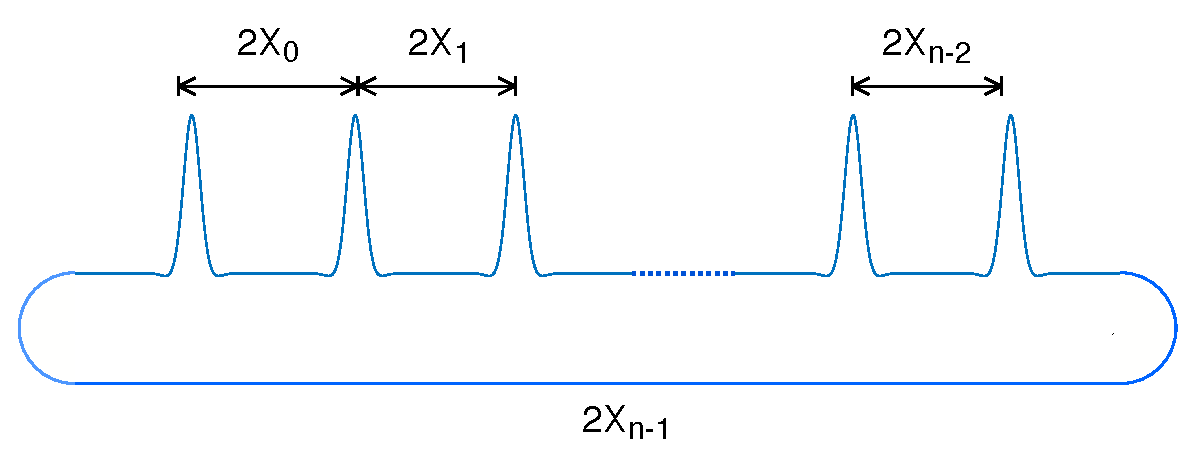
\includegraphics[width=10cm]{images/multipulseperiodic}
\end{center}
\caption[Construction of a periodic $n$-pulse solution]{Construction of a periodic $n-$pulse solution from the primary pulse.}
\label{fig:permultipulse}
\end{figure}
\noi A periodic $n$-pulse can be described by $n$ pulse distances $2 X_0, \dots, 2 X_{n-1}$, as shown in \cref{fig:permultipulse}. The period of the orbit is $2X$, where $X = X_0 + \dots + X_{n-1}$. A periodic $n$-pulse requires one more distance parameter than $n$-pulse on the real line, since we need one more connection to ``close the loop''.  Rather than describing a periodic multi-pulse by the ``physical'' pulse distances $X_i$, we will use a parameterization which is both more mathematically convenient and captures the underlying geometry necessary for a periodic $n$-pulse to exist. This parameterization is an adaptation of that in \cite{SandstedeStrut,Sandstede1998} to the periodic case. Let
\begin{equation}\label{defrho}
\rho = \frac{\beta_0}{\alpha_0}, \quad p^* = \arctan \rho
\end{equation}
where $\alpha_0$ and $\beta_0$ are defined in \cref{hyp:hypeq}. Define the set
\begin{align}
\mathcal{R} &= \left\{ \exp\left(-\frac{2 m \pi}{\rho}\right) : m \in \N_0 \right\} \cup \{ 0 \},
\end{align}
which is a complete metric space. We will use $r \in \mathcal{R}$ as a scaling parameter. The parameterization is defined as follows.

\begin{definition}\label{def:perparam}
For $n \geq 2$, a \emph{periodic parameterization} of a periodic $n$-pulse is a sequence $(m_0, \dots, m_{n-1}, \theta)$, where $\theta \in (-\pi + p^*, p^*]$ and $m_i$ is a nonnegative integer with
\begin{enumerate}[(i)]
\item at least one of the $m_i \in \{0, 1\}$
\item $m_{n-1} \geq m_i$ for $i = 0, \dots, n-2$.
\end{enumerate}
\end{definition}
\noi The selection of $m_{n-1}$ as the largest of the $m_i$ is made for notational convenience and to allow the parameterization to be unique. Since we are on a periodic domain, there is no loss of generality. The physical pulse distances $X_i$ are determined by these parameters and by the scaling parameter $r$. If $r = \exp\left(-\frac{2 m \pi}{\rho}\right)$, then
\begin{align*}
X_i &= \frac{1}{2 \beta_0}\big( (2 m + m_i)\pi + \theta^*(\theta; m_{n-1} - m_i)\big) + L_0 && i = 0, \dots, n-2  \\
X_{n-1} &= \frac{1}{2 \beta_0}\big( (2 m + m_{n-1})\pi + \theta \big) + L_0,
\end{align*}
where $L_0$ is a constant. 
The functions $\theta^*(\theta; m): [-\pi + p^*, p^*] \rightarrow \R$ are defined for all nonnegative integers $m$, are continuous in $\theta$, and have the following properties.
\begin{enumerate}[(i)]
\item $\theta^*(0; m) = 0 \text{ for all } m$
\item $|\theta^*(\theta; m)| \leq |\theta|$
\item $|\theta^*(\theta; m)| \leq C \exp\left(-\frac{m \pi}{\rho} \right)$
\item $\theta^*(\theta; 0) = \theta $
\item $\theta^*(p^*; m) = \theta^*(-\pi+p^*; m+1)$
\end{enumerate}
The last property is a matching condition which ``links up'' the parameterizations corresponding to adjacent $m_i$. \cref{fig:thetastarcartoon} shows a cartoon of first four $\theta^*(\theta; m)$ plotted consecutively to illustrate these properties. Together with the restriction of $\theta$ to the half-open interval $\theta \in (-\pi + p^*, p^*]$, these guarantee that each periodic parameterization corresponds to a unique periodic multi-pulse. The proof that the functions $\theta^*(\theta; m)$ exist and have these properties is given in Lemma \ref{thetaparamlemma} below.

\begin{figure}[H]
\begin{center}
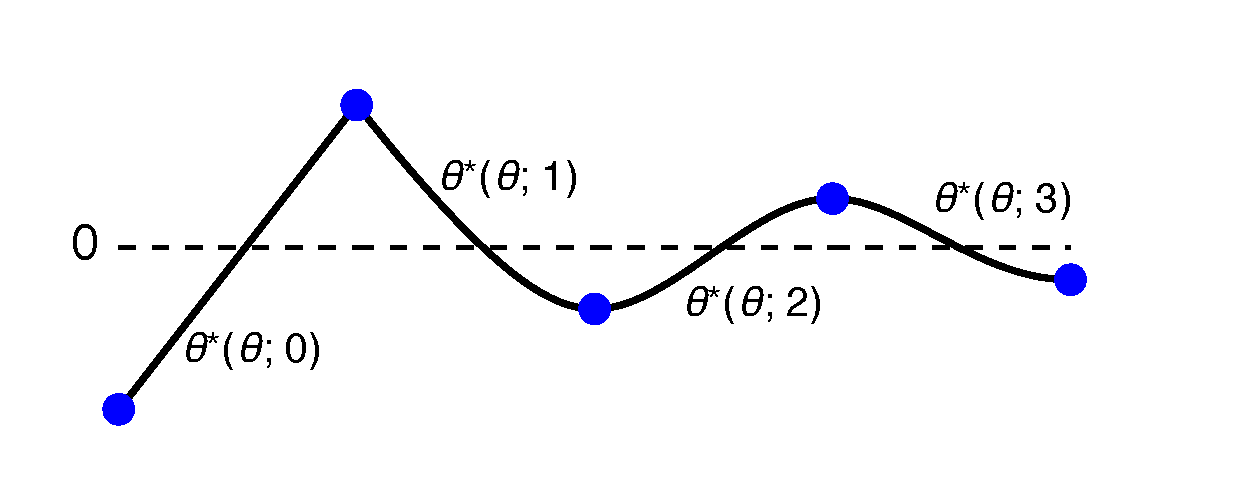
\includegraphics[width=12cm]{images/thetastarcartoon.eps}
\end{center}
\caption[Cartoon for $\theta^*(\theta; m)$]{Cartoon showing the first four functions $\theta^*(\theta; m)$ plotted consecutively. The region between each pair of blue dots corresponds to the domain $\theta = [-\pi + p^*, p^*]$.}
\label{fig:thetastarcartoon}
\end{figure} 

We can now state the main theorem of this section, which gives conditions for the existence of periodic multi-pulses. The requirement that the scaling parameter $r$ be sufficiently small means that the individual pulses must be well-separated. The proof is given in \cref{sec:existproof}. 

\begin{theorem}[Existence of $n$-periodic solutions]\label{th:perexist}
Assume Hypotheses \ref{hyp:E}, \ref{hyp:H}, \ref{hyp:hypeq}, \ref{Qexistshyp}, and \ref{hyp:transverse}. Let $Q_1(x)$ be the transversely constructed, symmetric primary pulse solution to \eqref{genODE} from \cref{transverseint}. For any periodic parameterization $(m_0, \dots, m_{n-1}, \theta)$ with $\theta \notin \{-\pi + p^*, p^* \}$, there exists $r_* = r_*(m_0, \dots, m_{n-1}, \theta) > 0$ such that for any $r \in \mathcal{R}$ with $r \leq r_*$, there exists a periodic $n$-pulse solution $U(x) = U(x; m_0, \dots, m_{n-1}, \theta, r)$ to \eqref{genODE}. The distances between consecutive copies of $Q_1(x)$ in $U(x)$ are $2X_i$, where
\begin{equation}\label{Xi}
\begin{aligned}
	X_i(r; m_i, m_{n-1},\theta) &= \frac{1}{2 \alpha_0} |\log r| + \frac{1}{2\beta_0} t_i(r; m_i,m_{n-1}, \theta) + L_0 && i = 0, \dots, n-2 \\
	X_{n-1}(r; m_{n-1}, \theta) &= \frac{1}{2 \alpha_0} |\log r| + \frac{1}{2 \beta_0}\big( m_{n-1}\pi + \theta \big) + L_0.
\end{aligned}
\end{equation}
The functions $t_i(r; m_i, m_{n-1}, \theta): \mathcal{R} \rightarrow \R$ are continuous in $r$ with 
\[
t_i(0; m_i, \theta) = m_i \pi + \theta^*(\theta; m_{n-1} - m_i) = m_i \pi + \mathcal{O}\left( e^{-\frac{\pi}{\rho}(m_{n-1} - m_i)} \right),
\]
and $L_0$ is a constant. Estimates for $U(x)$ in terms of the primary pulse $Q_1(x)$ are given below in Lemma \ref{solvewithjumps}.
\end{theorem}

\begin{remark}
It follows from the proof of \cref{2pulsebifurcation} that periodic single pulse solutions exist on domain $[-X, X]$ for all sufficiently large $X$. These are single-loop periodic orbits which lie close to the primary homoclinic orbit.
\end{remark}

The condition that $\theta \notin \{-\pi + p^*, p^* \}$ in \cref{th:perexist} is used to avoid bifurcation points which arise in the construction. For periodic 2-pulses, we can use the symmetry of the solutions to give a complete bifurcation picture. In the next theorem, we show that for periodic 2-pulses, asymmetric solutions ($X_0 \neq X_1$) bifurcate from symmetric solutions ($X_0 = X_1$) in a series of pitchfork bifurcations (\cref{fig:2pitch}, left panel). \cref{2pulsebifurcation} uses a different parameterization than \cref{th:perexist} (\cref{fig:2pitch}, right panel). The proof is given in \cref{sec:existproof}. 

\begin{figure}[H]
\begin{center}
\begin{tabular}{cc}
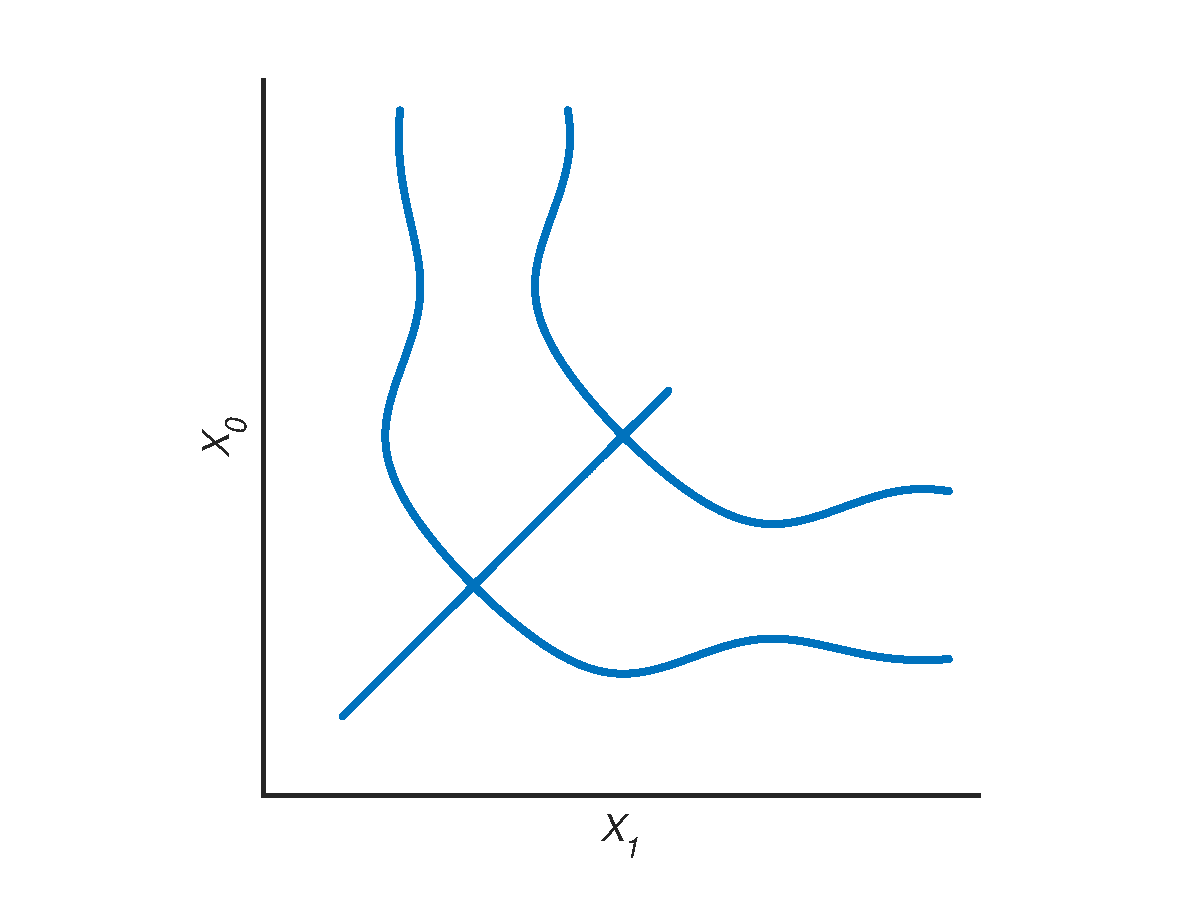
\includegraphics[width=8cm]{images/2pitchfork.eps}
\includegraphics[width=8cm]{images/2pitchparam1}
\end{tabular}
\end{center}
\caption[Pitchfork bifurcation structure for periodic 2-pulses]{Pitchfork bifurcation structure for periodic 2-pulses (right panel). Parameterization from \cref{2pulsebifurcation} (left panel). Blue represents symmetric periodic 2-pulses, and orange represents asymmetric periodic 2-pulses are in orange. Parameters $s_0$ and $s_1$ increase in the direction of the arrow.}
\label{fig:2pitch}
\end{figure} 

\begin{theorem}\label{2pulsebifurcation}
Assume Hypotheses \ref{hyp:E}, \ref{hyp:H}, \ref{hyp:hypeq}, \ref{Qexistshyp}, and \ref{hyp:transverse}. Let $Q_1(x)$ be the transversely constructed, symmetric primary pulse solution to \eqref{genODE} from Hypothesis \ref{Qexistshyp}. Then there exists $r_* > 0$ such that for all $r \in \mathcal{R}$ with $r \leq r_*$ and $m_0 \in \{0, 1\}$,
\begin{enumerate}[(i)]
	\item There exists a family of symmetric periodic 2-pulses $\tilde{Q}_2(x; m_0, s_0, r)$ parameterized by $s_0 \in [0, \pi)$. The pulse distances $\tilde{X}_i$ are given by
	\begin{equation}\label{2psymmdist}
		\tilde{X}_0(r, s_0) = \tilde{X}_1(r, s_0) = \frac{1}{2 \alpha_0} |\log r| + \frac{1}{2\beta_0} (m_0 \pi + s_0) + L_0.
	\end{equation}
	\item There exists a family of asymmetric periodic 2-pulses $Q_2(x; m_0, s_1, r)$ with distances $X_1 > X_0$ parameterized by $s_1 \in [p^*, \infty)$. The pulse distances $X_i$ are given by
	\begin{equation}\label{2pasymmdist}
	\begin{aligned}
		X_0(r, m_0, s_1) &= \frac{1}{2 \alpha_0} |\log r| + \frac{1}{2\beta_0} t_0(r; m_0, s_1) + L_0 \\
		X_1(r, s_1) &= \frac{1}{2 \alpha_0} |\log r| + \frac{1}{2\beta_0} s_1 + L_0, 
	\end{aligned}
	\end{equation}
	where $t_0(r; m_0, s_1)$ is continuous in $r$ and $s_1$, $t_0(0; m_0, k \pi) = m_0 \pi$ for all nonnegative integers $k$, and 
	\begin{align}\label{t0est}
	t_0(0; m_0, s_1) = m_0 \pi + \mathcal{O}\left(e^{-\frac{1}{\rho} s_1 }\right).
	\end{align}

	\item The two families meet at a pitchfork bifurcation when $s_0 = p^*(m_0; r)$ and $s_1 = p^*$, where $p^*(m_0; r)$ is continuous in $r$, and $p^*(m_0; r) \rightarrow p^*$ as $r \rightarrow 0$.
\end{enumerate}
\end{theorem}

\section{Spectrum of periodic multi-pulses}\label{sec:perstab}

We now look at the spectrum of the periodic multi-pulses which we constructed in the previous section. Let $Q_n(x) = (q_n(x), \partial_x q_n(x), \dots, \partial_x^{2m} q_n(x), 0)$ be any periodic $n$-pulse solution constructed according to \cref{th:perexist} on periodic domain $[-X, X]$. It is natural to pose the PDE eigenvalue problem \cref{genPDEeig2} on the space of periodic functions $H^{2m}_{\text{per}}[-X,X]$, where
\[
H^{2m}_{\text{per}}[-X,X] = \left\{ f \in H^{2m}(\R) : f^{(k)}(-X) = f^{(k)}(X) \text{ for } k = 0, \dots, 2m \right\},
\]
although we note that in doing so, we are restricting ourselves to co-periodic perturbations. By \cref{Ekernel}, $\partial_x \calL(q_n)$ has a kernel with algebraic multiplicity at least 2 and geometric multiplicity at least 1. In the next lemma, we show that there is another kernel eigenfunction when the eigenvalue problem is posed on $H^{2m}_{\text{per}}[-X,X]$. 

\begin{lemma}\label{qnkernel}
The linear operator $\partial_x \calL(q_n)$ on $H^{2m}_{\text{per}}[-X,X]$ has a kernel eigenfunction $v_n^c$, which is a solution to $\calL(q_n)v_n^c = 1$.
\begin{proof}
Since $1 \in H^{2m}_{\text{per}}[-X,X]$, $\calL(q_n) 1 = c \neq 0$, and $\calL(q_n)$ is self-adjoint, for any $v \in \ker \calL(q_n)$,
\begin{align*}
\langle 1, v \rangle = \frac{1}{c} \langle \calL(q_n) 1, v \rangle
= \frac{1}{c} \langle  1, \calL(q_n)^* v \rangle = \frac{1}{c} \langle  1, \calL(q_n) v \rangle = 0,
\end{align*}
thus $1 \perp \ker \calL(q_n)^*$. By the Fredholm alternative, the equation $\calL(q_n) v_n^c = 1$ has a solution $v_n^c \in H^{2m}_{\text{per}}[-X,X]$. Differentiating with respect to $x$, $\partial_x \calL(q_n) v_n^c = 0$.
\end{proof}
\end{lemma}

\noi Using a spatial dynamics approach from \cref{sec:EVP}, the PDE eigenvalue problem on $H^{2m}_{\text{per}}[-X,X]$ is equivalent to the first order system with periodic boundary conditions
\begin{equation}\label{PDEeigsystemper3}
\begin{aligned}
V'(x) &= A(Q_n(x))V(x) + \lambda B V(x) \\
V(-X) &= V(X),
\end{aligned}
\end{equation}
where $V(x) \in C^0(\R,\R^{2m+1})$. Let $A(\lambda) = A(0) + \lambda B$. In next lemma we show that for small $\lambda$, $A(\lambda)$ has a simple eigenvalue $\nu(\lambda)$ near 0.

\begin{lemma}\label{nulambdalemma}
There exists $\delta_1 > 0$ such that for $|\lambda| < \delta_1$, the matrix $A(\lambda)$ has a simple eigenvalue $\nu(\lambda)$. $\nu(\lambda)$ is smooth in $\lambda$, $\nu(0) = 0$, $\nu'(0) = 1/c$, and for $|\lambda| < \delta_1$,
\begin{equation}\label{nulambda}
\nu(\lambda) = \frac{1}{c} \lambda + \mathcal{O}(|\lambda|^3)
\end{equation}
In addition, $\nu(-\lambda) = -\nu(\lambda)$ and $\nu(\overline{\lambda}) = \overline{\nu(\lambda)}$.
\begin{proof}
Let $p(\nu; \lambda)$ be the characteristic polynomial of $A(\lambda)$. Since $p(0; 0) = 0$ and $\partial_\nu p(0; 0) = -c \neq 0$, by the implicit function theorem there exists $\delta_1 > 0$ and a smooth function $\nu(\lambda)$ such that $\nu(0) = 0$ and for $|\lambda| < \delta_1$, $\nu(\lambda)$ is the unique solution to $p(\nu; \lambda) = 0$, and $\nu'(0) = 1/c$. By reversibility, $p(\nu; \lambda)$ only involves odd powers of $\nu$, thus $p(\nu; \lambda) = 0$ if and only if $p(-\nu; -\lambda) = 0$. Since the solution $\nu(\lambda)$ is unique, $\nu(-\lambda) = -\nu(\lambda)$. Conjugate symmetry follows similarly since $p(\nu; \lambda) = 0$ if and only if $p(\overline{\nu}; \overline{\lambda}) = 0$. Equation \cref{nulambda} follows from a Taylor expansion of $\nu(\lambda)$ about $\lambda = 0$. 
\end{proof}
\end{lemma}

We can now state the main theorem of this section, which provides a condition for \cref{PDEeigsystemper3} to have a solution. Since the spatial dynamics formulation \cref{PDEeigsystemper3} is equivalent to the PDE eigenvalue problem, this allow us to find the eigenvalues of \cref{genPDEeig2}. This theorem is analogous to \cite[Theorem 2]{Sandstede1998}, with the $n\times n$ matrix in that theorem replaced by a $2n\times 2n$ block matrix. The proof is given in \cref{sec:blockmatrixproof}.

% block matrix theorem
\begin{theorem}\label{blockmatrixtheorem}
Assume Hypotheses \ref{hyp:E}, \ref{hyp:H}, \ref{hyp:hypeq}, \ref{Qexistshyp}, and \ref{hyp:transverse}, and \ref{hyp:dccpos}. Let $Q_1(x)$ be the transversely constructed, symmetric primary pulse solution to \eqref{genODE} from \cref{Qexistshyp}, and let $Q(x) = (Q_1(x), 0)$. Let $\Psi(x)$ and $V^c(x)$ be defined as in \cref{varadjsolutions}. Choose any periodic parameterization $(m_0, \dots, m_{n-1}, \theta)$ with $\theta \notin \{-\pi + p^*, p^* \}$. Let $r_*$ be defined as in \cref{th:perexist}, and for $r \leq r_*$, let $Q_n(x; r)$ be the corresponding periodic $n$-pulse solution. Then there exists $r_1 \leq r_*$ and $\delta > 0$ with the following property. For $r \leq r_1$, there exists a bounded, nonzero solution $V(x)$ of \cref{PDEeigsystemper3} for $|\lambda| < \delta$ and $|\Re \lambda| < r^{1/4}$ if and only if
\begin{equation}\label{blockmatrixcond}
E(\lambda) = \det S(\lambda) = 0.
\end{equation}
$S(\lambda)$ is the $2n \times 2n$ block matrix
\begin{equation}\label{blockeq}
S(\lambda) = 
\begin{pmatrix}
K(\lambda) - \frac{1}{2} \lambda \tilde{M} K^+(\lambda) & \lambda^2 M_c I \\
-\frac{1}{2} \lambda M_c K^+(\lambda) & A - \lambda^2 MI 
\end{pmatrix} +
\begin{pmatrix}C_1 & D_1 \\ C_2 & D_2
\end{pmatrix},
\end{equation}
and the individual terms in $S(\lambda)$ are as follows.

\begin{enumerate}[(i)]
\item $K(\lambda)$ is the periodic, bi-diagonal matrix
\begin{align*}
K(\lambda) &=  
\begin{pmatrix}
e^{-\nu(\lambda)X_1} & -e^{\nu(\lambda)X_0} \\
-e^{\nu(\lambda)X_1} & e^{-\nu(\lambda)X_0} \\
\end{pmatrix} && n = 2\\
K(\lambda) &=  
\begin{pmatrix}
e^{-\nu(\lambda)X_1} & & & & & -e^{\nu(\lambda)X_0} \\
-e^{\nu(\lambda)X_1} & e^{-\nu(\lambda)X_2} \\
& -e^{\nu(\lambda)X_2} & e^{-\nu(\lambda)X_3} \\
  & & \ddots & && \\
& & & & -e^{\nu(\lambda)X_{n-1}} & e^{-\nu(\lambda)X_0}
\end{pmatrix} && n > 2,
\end{align*}
where $\nu(\lambda)$ is defined in Lemma \ref{nulambdalemma}. $K^+(\lambda)$ is the same matrix as $K(\lambda)$ with all terms positive.

\item $A$ is the symmetric banded matrix
\begin{align}\label{Asymm}
A &= \begin{pmatrix}
-a_1 - a_0 & a_1 + a_0 \\
a_1 + a_0 & - a_1 - a_0 
\end{pmatrix} && n = 2 \\
A &= \begin{pmatrix}
-a_{n-1} - a_0 & a_0 & & &  & a_{n-1}\\
a_0 & -a_0 - a_1 &  a_1 \\
& a_1 & -a_1 - a_2 &  a_2 \\
& \ddots & \ddots & \ddots \\
a_{n-1} & & & & a_{n-2} & -a_{n-2} - a_{n-1} \\
\end{pmatrix} && n > 2,
\end{align}
where
\begin{align*}
a_i &= \langle \Psi(X_i), Q'(-X_i) \rangle
\end{align*}

\item $M$, $M_c$, and $\tilde{M}$ are the Melnikov-type integrals
\begin{align*}
M &= \int_{-\infty}^\infty q(y) \partial_c q(y) dy, \quad
M_c = \int_{-\infty}^\infty \partial_c q(y) dy, \quad
\tilde{M} = \int_{-\infty}^{\infty} \left(v^c(y) - \frac{1}{c}\right) dy,
\end{align*}
where $v^c(y)$ is the first component of $V^c(y)$, and $q(y)$ is the first component of $Q(y)$.

\item The remainder matrices $C_i$ and $D_i$ are analytic in $\lambda$ and have uniform bounds
\begin{align*}
|C_1| &\leq C (|\lambda| + r^{1/2})^2, \quad
|D_1| \leq C |\lambda|(|\lambda| + r^{1/2})^2 \\
|C_2| &\leq C (|\lambda| + r^{1/2})^2, \quad
|D_2| \leq C (|\lambda| + r^{1/2})^3 
\end{align*}
\end{enumerate}
\end{theorem}

The condition $|\Re \lambda| < r^{1/4}$ is used to simplify the analysis. We will see in \cref{sec:perdouble} that this condition is satisfied for sufficiently small $r$.

\subsection{Spectrum of periodic single pulse}\label{sec:persingle}

The simplest case is the periodic single pulse. There is a only single length parameter $X_0$, which is the same as the domain length $X$, and the block matrix $S(\lambda)$ is a $2\times 2$ matrix. The form of $S(\lambda)$ is given in the following lemma. Proofs of all results in this section are given in \cref{sec:singlepulse}. 

\begin{lemma}\label{lemma:1blockmatrix}
For a periodic single pulse, the block matrix $S(\lambda)$ from \cref{blockmatrixtheorem} is 
\begin{align}\label{1pblockmatrix}
S(\lambda) &= 
\begin{pmatrix}
-2 \sinh(\nu(\lambda) X) - \tilde{M}\lambda \cosh(\nu(\lambda) X) & M_c \lambda^2 \\
-M_c \lambda \cosh(\nu(\lambda)X) & - M \lambda^2
\end{pmatrix} +
\begin{pmatrix}
c_1 & d_1 \\ c_2 & d_2
\end{pmatrix},
\end{align}
where the remainder terms are scalars with bounds
\begin{align*}
|c_1|, |c_2| &\leq C |\lambda|(|\lambda| + r^{1/2}), \qquad |d_1|, |d_2| \leq C |\lambda|^2(|\lambda| + r^{1/2}).
\end{align*}
In addition, $\det S(-\lambda) = -\det S(\lambda)$, and 
\begin{equation}\label{1pblockmatrixdet}
\begin{aligned}
\det S(\lambda, r) &= \lambda^2 \Big( 2 M \sinh(\nu(\lambda)X)(1 + \mathcal{O}(|\lambda| + r^{1/2} )) + \lambda(M \tilde{M} + M_c^2 )\cosh(\nu(\lambda)X) + \mathcal{O}(|\lambda|(|\lambda| + r^{1/2} ) \Big),
\end{aligned}
\end{equation}
\end{lemma}

\noi Using this lemma, we can compute the nonzero essential spectrum eigenvalues for the periodic single pulse.

\begin{theorem}\label{theorem:1pess}
Assume Hypotheses \ref{hyp:E}, \ref{hyp:H}, \ref{hyp:hypeq}, \ref{Qexistshyp}, and \ref{hyp:transverse}, and \ref{hyp:dccpos}. Let $r_*$ be as in \cref{th:perexist}, and let $\delta(r)$ be as in Theorem \ref{blockmatrixtheorem}. Then there exists $r_1 \leq r_*$ such that for any $r \in \mathcal{R}$ with $r \leq r_1$, the following holds regarding the nonzero essential spectrum eigenvalues. Let $N$ be any positive integer such that $\frac{N \pi}{X} < \delta(r)$. Then there are $2N$ nonzero essential spectrum eigenvalues $\lambda = \{ \pm \lambda_m^{\text{ess}} : m = 1, \dots, N \}$, where
\begin{align}\label{1pess}
\lambda_m^{\text{ess}}(r) = c \frac{m \pi i}{X + c \frac{M\tilde{M} + M_c^2 }{2 M}} +  \mathcal{O}\left( \frac{m^3}{|\log r|^3} \right)
\end{align}
is on the imaginary axis.
\end{theorem}

\subsection{Spectrum of periodic double pulse}\label{sec:perdouble}

Next, we consider the periodic double pulse. In this case, the block matrix $S(\lambda)$ is a $4\times 4$ matrix, the form of which is given in the next lemma. Proofs of all results in this section are given in \cref{sec:doublepulse}. 

\begin{lemma}\label{lemma:2blockmatrix}
For a periodic 2-pulse, the block matrix $S(\lambda)$ from \cref{blockmatrixtheorem} is the $4 \times 4$ matrix
\begin{align}\label{dpSmatrix}
S(\lambda) = 
\begin{pmatrix}
e^{-\nu(\lambda)X_1} -\frac{1}{2}\lambda \tilde{M} e^{-\nu(\lambda)X_1} & -e^{\nu(\lambda)X_0} -\frac{1}{2}\lambda \tilde{M} e^{\nu(\lambda)X_0} & M_c \lambda^2 & 0 \\
-e^{\nu(\lambda)X_1} -\frac{1}{2}\lambda \tilde{M} e^{\nu(\lambda)X_1} & e^{-\nu(\lambda)X_0} -\frac{1}{2}\lambda \tilde{M} e^{-\nu(\lambda)X_0} & 0 & M_c \lambda^2 \\
-\frac{1}{2}\lambda M_c e^{-\nu(\lambda)X_1} & -\frac{1}{2}\lambda M_c e^{\nu(\lambda)X_0} &-a-\lambda^2 M & a \\
-\frac{1}{2}\lambda M_c e^{\nu(\lambda)X_1} & -\frac{1}{2}\lambda M_c e^{-\nu(\lambda)X_0}  & a & -a-\lambda^2 M
\end{pmatrix} + R(\lambda)
\end{align}
where
\begin{equation}\label{2pa}
a = \langle \Psi(X_0), Q'(-X_0) \rangle + \langle \Psi(X_1), Q'(-X_1) \rangle.
\end{equation}
The remainder matrix is a $4 \times 4$ matrix of the form
\begin{align}
R(\lambda) = 
\begin{pmatrix} 
c_1(\lambda) & \tilde{c}_1(\lambda) & \lambda d_1(\lambda) & \lambda \tilde{d}_1(\lambda) \\ 
-c_1(-\lambda) & -\tilde{c}_1(-\lambda) & -\lambda \tilde{d}_1(-\lambda) & -\lambda d_1(-\lambda) \\ 
c_2(\lambda) & \tilde{c}_2(\lambda) & d_0 + \lambda d_2(\lambda) & -d_0 + \lambda \tilde{d}_2(\lambda) \\ 
-c_2(-\lambda) & -\tilde{c}_2(-\lambda) & -d_0 - \lambda \tilde{d}_2(-\lambda) & d_0 - \lambda d_2(-\lambda)
\end{pmatrix},
\end{align}
where the individual entries have bounds
\begin{align*}
|d_0| &\leq C r^{3/2} \\
|c_i|, |\tilde{c}_i|, |d_i|, |\tilde{d}_i| &\leq C (|\lambda| + r^{1/2})^2 && i = 1, 2
\end{align*}
In addition,
\begin{equation}\label{2pblockmatrixdet}
\begin{aligned}
\det S(&\lambda, r) = -2 \lambda^2 (2a + \lambda^2 M + R_1) \left( M \sinh(\nu(\lambda)X) + \lambda (M \tilde{M} + M_c^2 ) \cosh(\nu(\lambda)X) \right) \\
&+4 a \lambda^3 M_c^2 \sinh(\nu(\lambda)X_1)\sinh(\nu(\lambda)X_0) 
+ R_2 \lambda^2 \sinh(\nu(\lambda)(X_1 - X_0)) + \lambda^2 R_3 \sinh(\nu(\lambda)X)) + \lambda^3 R_4,
\end{aligned}
\end{equation}
where the $R_i$ are scalars with bounds 
\begin{equation*}
|R_1| \leq C r^{3/2}, \quad |R_2|, |R_3|, |R_4| \leq C(|\lambda| + r^{1/2})^4,
\end{equation*}
and $\det S(-\lambda) = -\det S(\lambda)$.
\end{lemma}

We will consider first the case where the interaction eigenvalues are ``out of the way'' of the essential spectrum eigenvalues. Since the interaction eigenvalues scale as $r^{1/2}$ and the essential spectrum eigenvalues scale as $1/|\log r|$, we can always choose $r$ sufficiently small so that this is the case. We will state the result separately for asymmetric and symmetric periodic 2-pulses. First, we locate the eigenvalues for asymmetric periodic 2-pulses. As long as $r$ is chosen sufficiently small, the interaction eigenvalue pattern is determined by the parameter $m_0$, and the essential spectrum eigenvalues do not interfere.

\begin{theorem}\label{theorem:2peigsassym}
Assume Hypotheses \ref{hyp:E}, \ref{hyp:H}, \ref{hyp:hypeq}, \ref{Qexistshyp}, and \ref{hyp:transverse}, and \ref{hyp:dccpos}. Let $r_*$ be as in \cref{2pulsebifurcation}, and let $\delta(r)$ be as in Theorem \ref{blockmatrixtheorem}. Then for every $m_0 \in \{0, 1\}$ and $s_1 > p^*$ there exists $r_1 = r_1(m_0, s_1) \leq r_*$ such that for any $r \in \mathcal{R}$ with $r \leq r_1$, the following hold regarding the spectrum associated with the asymmetric periodic 2-pulse $Q_2(x; m_0, s_1, r)$.

\begin{enumerate}[(i)]
\item Let $N$ be any positive integer such that $\frac{N \pi}{X} < \delta(r)$. Then there are $2N$ nonzero essential spectrum eigenvalues $\lambda = \{ \pm \lambda_m^{\text{ess}} : m = 1, \dots, N \}$, where
\begin{align}\label{2pess}
\lambda_m^{\text{ess}}(r) = c \frac{m \pi i}{X + c \frac{M\tilde{M} + M_c^2}{M}} +  \mathcal{O}\left( \frac{m^3}{|\log r|^3} \right)
\end{align}
is on the imaginary axis.

\item There is a pair of interaction eigenvalues located at $\lambda = \pm \lambda^{\text{int}}(r)$, where
\begin{align*}
\lambda^{\text{int}}(r) = \sqrt{-\frac{2a}{M}} + \mathcal{O}\left( r \right).
\end{align*}
$a$ is defined in \cref{2pa} and $|\lambda^{\text{int}}(r)| < \frac{1}{2}|\lambda_1^{\text{ess}}(r)|$. These are real when $m_0 = 0$ and purely imaginary when $m_0 = 1$.
\item There is an eigenvalue at 0 with algebraic multiplicity 3. 
\item There are no other eigenvalues inside a circle with radius slightly larger than $|\lambda_{N}^{\text{ess}}(r)|$.
\end{enumerate}
\end{theorem}

We note that the interaction eigenvalues are order $r^{1/2}$ and the essential spectrum eigenvalues are purely imaginary, thus the condition $|\Re \lambda| < r^{1/4}$ is satisfied for sufficiently small $r$.

\begin{remark}The essential spectrum eigenvalues are not identical for the periodic single pulse and the periodic double pulse. In particular, note the additional factor of 2 in the denominator of \cref{1pess}.
\end{remark}

Next, we consider the symmetric periodic 2-pulse. As long as we are away from the pitchfork bifurcation points, i.e. as long as $a \neq 0$, the results of \cref{theorem:2peigsassym} hold in the symmetric case as well; the only difference is that the eigenvalue pattern is determined by the sign of $a$ rather than by $m_0$ (see \cref{lemma:chara} below). Thus we only need to consider what happens at the pitchfork bifurcation point.

\begin{theorem}\label{theorem:2peigssym}
Assume Hypotheses \ref{hyp:E}, \ref{hyp:H}, \ref{hyp:hypeq}, \ref{Qexistshyp}, and \ref{hyp:transverse}, and \ref{hyp:dccpos}. Then there exists $r_1 \leq r_*$ such that for all $r \in \mathcal{R}$ with $r \leq r_1$ and for $m_0 \in \{0, 1\}$, there is eigenvalue at 0 with algebraic multiplicity 5 for the symmetric periodic 2-pulse $\tilde{Q}_2(x; m_0, p^*(m_0; r), r)$, where $p^*(m_0; r)$ is defined in \cref{2pulsebifurcation}.
\end{theorem}

Finally, we consider what happens when essential spectrum eigenvalues collide with an interaction eigenvalue on the imaginary axis. For simplicity, we will only show what happens for the first collision. The existence of the first Krein bubble is given in the following theorem, which also provides numerically verifiable estimates for its size and location. 

\begin{theorem}\label{th:Kreinbubble}
Assume Hypotheses \ref{hyp:E}, \ref{hyp:H}, \ref{hyp:hypeq}, \ref{Qexistshyp}, and \ref{hyp:transverse}, and \ref{hyp:dccpos}. Choose $m_0 = 1$, and let $r_*$ be as in \cref{2pulsebifurcation}. Let 
\begin{align}\label{deflambdastar}
\lambda_*(r) &= \sqrt{ \frac{-2a(r) - R_1 }{M} } + \mathcal{O}(r) = \sqrt{ \frac{-2a(r)}{M} } + \mathcal{O}(r),
\end{align}
and let $Q_2^*(x; r)$ be the periodic 2-pulse solution from \cref{2pulsebifurcation} with domain length $X = X_*(r)$, where
\begin{align}\label{defXstar}
X_*(r) &= c \left( \frac{\pi i}{\lambda_*(r)} - \frac{M \tilde{M} + M_c^2 }{M}\right).
\end{align}
Define $T_1(r) > 0$ by 
\begin{align}\label{defT0}
T_1(r) = \frac{M_c^2 }{2 \pi M^2 c } |\lambda_*|^5 X_0^2.
\end{align}
For $s \in [-2\sqrt{T_1(r)}, 2 \sqrt{T_1(r)}]$, let $Q_2(x; s, r)$ be the periodic 2-pulse solution with domain size $X = X(s, r)$, where
\begin{equation}
X(s,r) = X_*(r) + \frac{2 c \pi s}{|\lambda_*(r)|^2} + \mathcal{O}(s^2).
\end{equation}
Then there exists $r_0 \leq r_*$ such that the following holds for the linearization about $Q_2(x; s, r)$.
\begin{enumerate}[(i)]
	\item There is a pair of eigenvalues located at
	\begin{align}\label{Kreineigs}
	\lambda = \lambda_*(r) - s i \pm \sqrt{ T_1(r) -  s^2} + \mathcal{O}\left(r^{5/4}|\log r|^{1/2} \right)
	\end{align}

	\item For
	\[
	s = s_\pm(r) = \pm \sqrt{T_1(r)} + \mathcal{O}\left(r^{5/4}|\log r|^{1/2} \right),
	\]
	there is a double eigenvalue on the imaginary axis at $\lambda = \lambda_*(r) + s_\pm(r) i + \mathcal{O}\left(\frac{1}{|\log r|} \right)$, which occurs when 
	\begin{equation}\label{KreinDeltaX}
	X(s, r) = X_*(r) \pm \Delta X_1(r) + \mathcal{O}(s^2), \qquad \Delta X_1(r) = \frac{2 c \pi}{|\lambda_*(r)|^2}\sqrt{T_1(r)} 
	\end{equation}
\item For $s \in (s_-, s+)$, equation \cref{Kreineigs} describes, to leading order, a circle of radius $\sqrt{T_1(r)}$ in the complex plane, and the pair of eigenvalues is symmetric across the imaginary axis.
\item For $s \in [-2\sqrt{T_1(r)}, s_-) \cup (s_+, 2 \sqrt{T_1(r)}]$, the eigenvalues \cref{Kreineigs} are on the imaginary axis.
\end{enumerate}
\end{theorem}

We note that maximum real part of the Krein bubble is order $r^{5/4}|\log r|$, thus the condition $|\Re \lambda| < r^{1/4}$ is satisfied for sufficiently small $r$.

\begin{remark}\label{remark:kreinbubbles}
It is straightforward to adapt \cref{th:Kreinbubble} to locate more Krein bubbles. For any positive integer $N$, there exists $r_0 \leq r_*$ such that for $m = 1, \dots, N$, a Krein bubble occurs when the $m$-th essential spectrum eigenvalue collides with the interaction eigenvalue on the imaginary axis. The radius of $m$-th Krein bubble in the complex plane is approximately $\sqrt{T_1(r) / m}$, and the Krein collisions occur at approximately $X = X^m_*(r) \pm \Delta X^m(r)$, where 
\[
X^m_*(r) = c \left( \frac{m \pi i}{\lambda_*(r)} - \frac{M \tilde{M} + M_c^2 }{M}\right), \qquad \Delta X^m(r) = \sqrt{m} \Delta X_1(r).
\]
\end{remark}

\section{Numerical Results}\label{sec:numerics}

In this section, we present numerical results for the existence and spectrum of periodic multi-pulse solutions to KdV5. We start with the construction of the primary pulse solution. For $p = -1$ and $c = 36/169$, the exact solution to \cref{KdV5eq4} is known \cite[(3)]{Pelinovsky2007}
\begin{equation}\label{KdV5exactsol}
q(x) = \frac{105}{338}\sech^4\left(\frac{x}{2\sqrt{13}} \right).
\end{equation}
We use AUTO for parameter continuation in $c$ and $p$ until $-2 \sqrt{c} < p < 2 \sqrt{c}$, so that \cref{hyp:hypeq} is satisfied. Following the AUTO demo \texttt{kdv}, we formulate the problem using \cref{KdV5ham2} with a small parameter $\epsilon$ to break the Hamiltonian structure. We impose periodic boundary conditions and rescale the domain from $[-X, X]$ to $[0, 1]$, using the domain size $X$ as a parameter. 

To construct a periodic double pulse $q_2(x)$, we discretize equation \cref{KdV5eq4} using Fourier spectral differentiation matrices to enforce periodic boundary conditions. As an initial ansatz, we take two copies of the primary pulse spliced together at the distances predicted by \cref{2pulsebifurcation}. We then solve for the periodic double pulse using Matlab's \texttt{fsolve} function. This same procedure can also be used to construct arbitrary periodic multi-pulses. We can also vary the domain size $X$ by parameter continuation in AUTO, from which verify that asymmetric solutions bifurcate from symmetric solutions in a series of pitchfork bifurcations (\cref{fig:KdV5eigs1}, left panel). Next, we compute the spectrum of $\partial_x \calE''(q_n)$ by discretizing the linear operator using Fourier spectral differentiation matrices and using Matlab's \texttt{eig} function (\cref{fig:KdV5eigs1}). 
\begin{figure}[H]
\begin{center}
\begin{tabular}{cc}
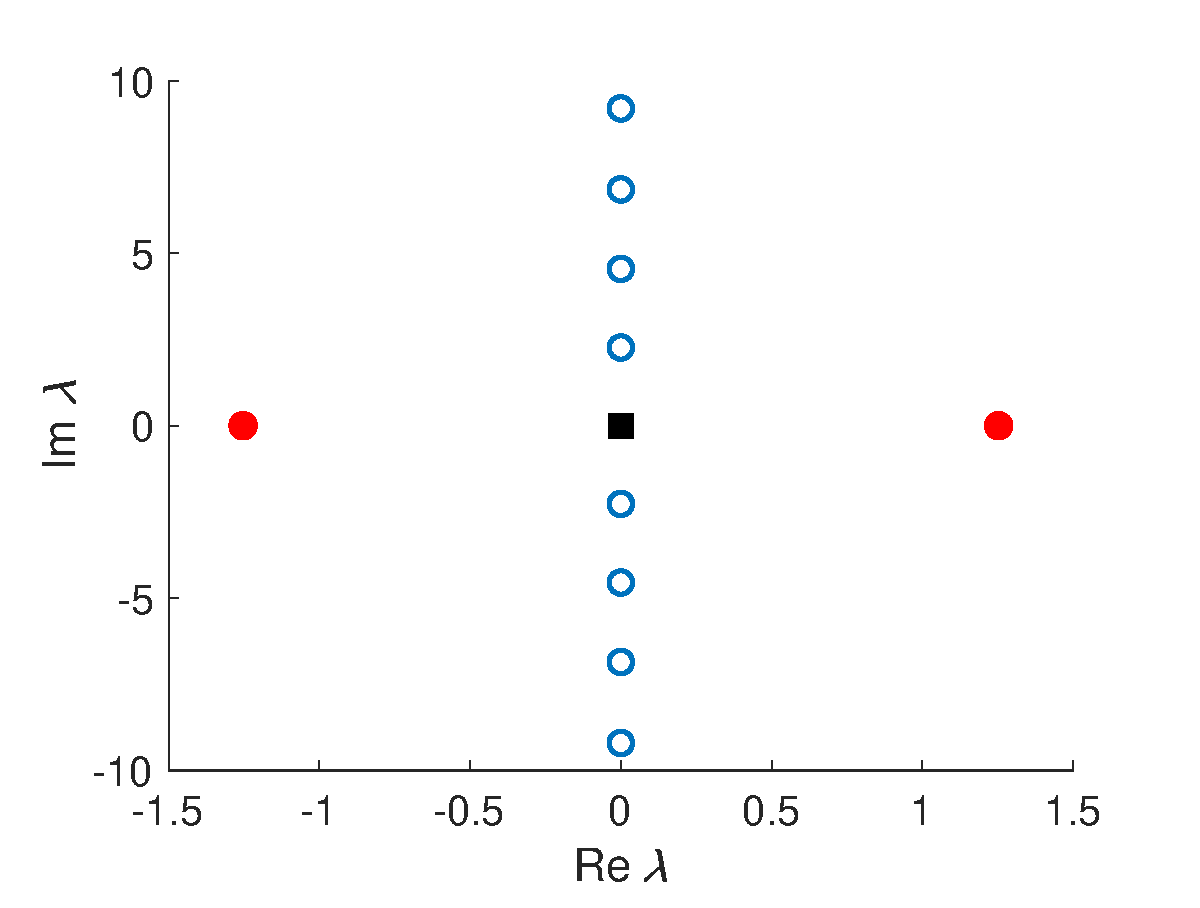
\includegraphics[width=7.5cm]{images/dp1spec.eps} &
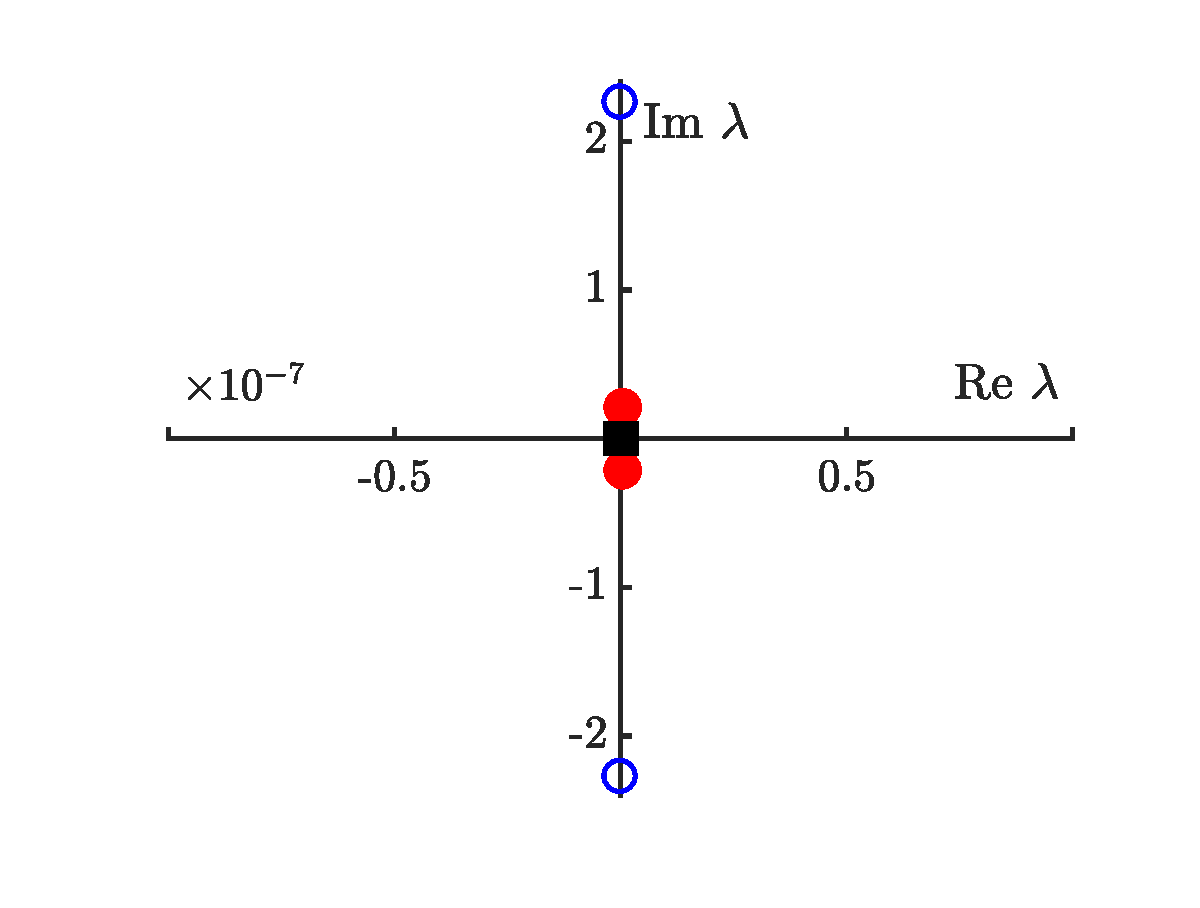
\includegraphics[width=7.5cm]{images/dp2spec.eps}
\end{tabular}
\end{center}
\caption[Spectrum of double pulse solutions]{Spectrum of first two double pulse solutions for KdV5, $X = 30$. Left panel ($m_0 = 0$) has real interaction eigenvalues, right panel ($m_0 = 1$) has imaginary eigenvalues. Interaction eigenvalues in red, essential spectrum eigenvalues in blue, kernel eigenvalues in black. Fourier spectral methods with $N = 1024$ grid points, $p = -1$, $c = 10$, $X = 30$.}
\label{fig:KdV5eigs1}
\end{figure}
For $m_0 = 1$ and $r$ sufficiently small, the interaction eigenvalues are purely imaginary; the real part of the eigenvalues computed with \texttt{eig} is order $10^{-9}$. We can also compute the interaction eigenvalues for symmetric periodic double pulses with equal pulse distances (\cref{fig:periodiceigbif}, right panel), which shows that at each pitchfork bifurcation point, an eigenvalue bifurcation occurs, where a pair of interaction eigenvalues collides at 0 and switches from real to purely imaginary (or vice versa). The full interaction eigenvalue pattern (up to the first Krein bubble) is shown in the left panel of \cref{fig:periodiceigbif}.
\begin{figure}[H]
\begin{center}
\begin{tabular}{cc}
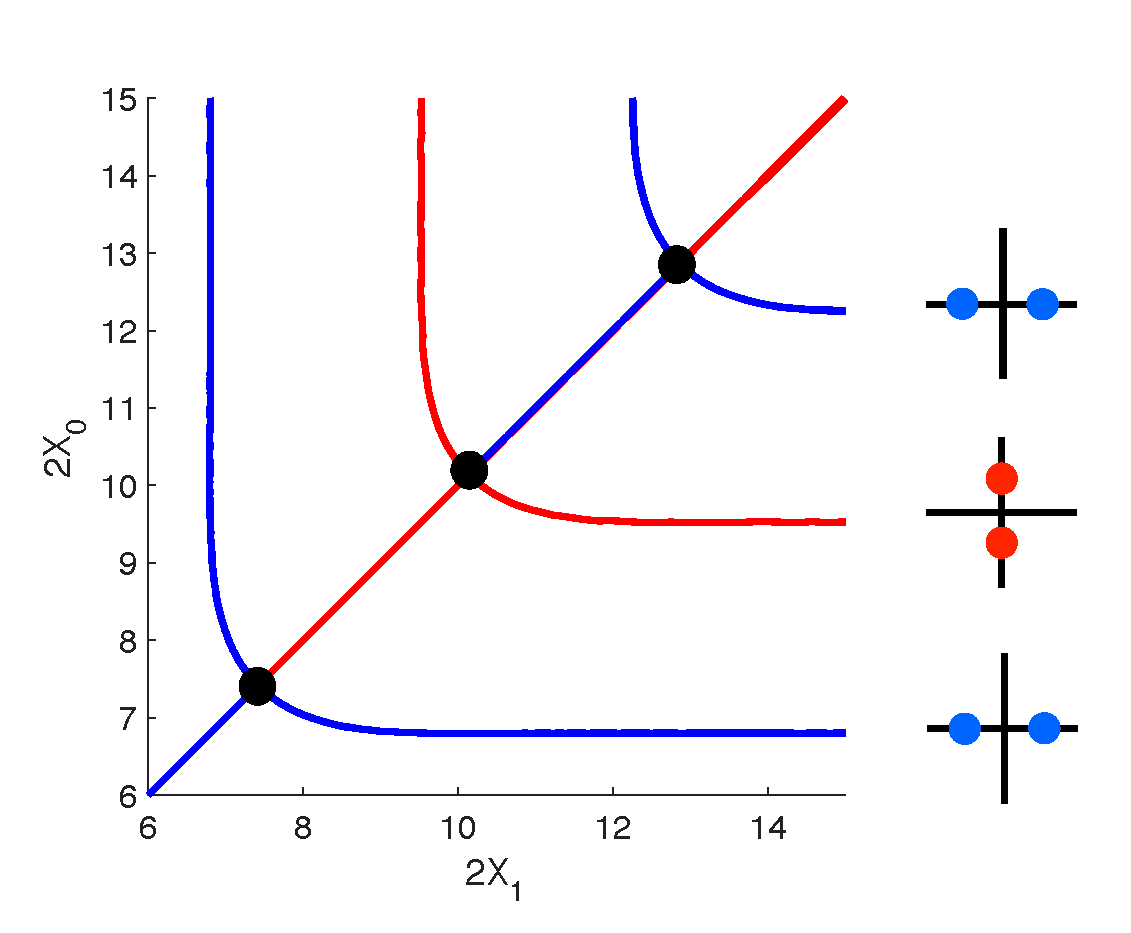
\includegraphics[width=7.5cm]{images/2periodiceigpattern.eps}
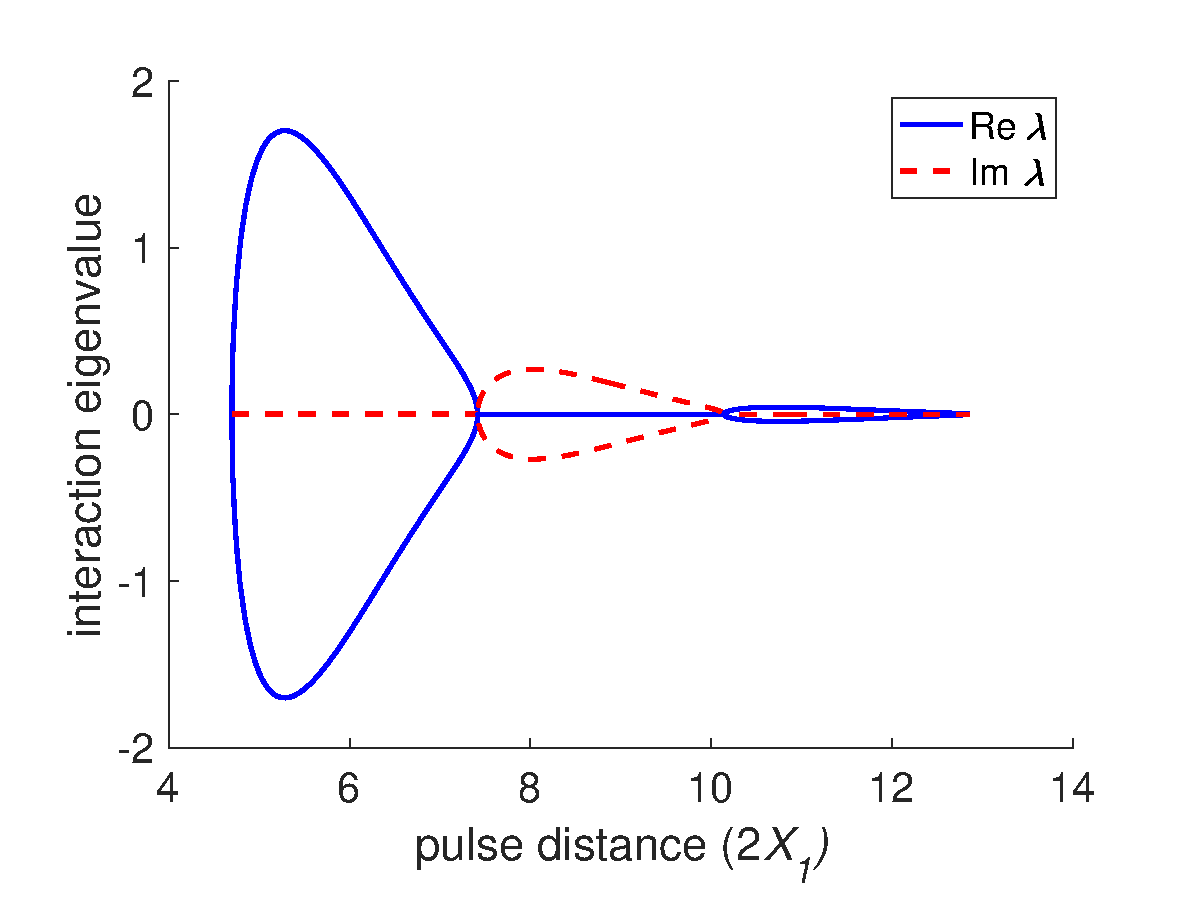
\includegraphics[width=7.5cm]{images/periodicequaleigbif.eps}
\end{tabular}
\end{center}
\caption{Right panel shows pitchfork bifurcation structure for periodic double pulses, as well as interaction eigenvalue pattern. Blue lines represent real interaction eigenvalues, and red lines represent purely imaginary interaction eigenvalues. Eigenvalue bifurcations take place at the pitchfork bifurcation points. Right panel shows real part (blue line) and imaginary part (red line) of interaction eigenvalues versus pulse distance for symmetric periodic double pulses. }
\label{fig:periodiceigbif}
\end{figure}
For the essential spectrum eigenvalues for periodic single and double pulses, we compare the results from \texttt{eig} to those predicted by the leading order formulas from \cref{theorem:1pess} and \cref{theorem:2peigsassym}. Plotting the log of absolute value of the error vs $\log m$ and constructing a least squares linear regression line (\cref{fig:DP2esslogerror}), the absolute error is proportional to $m^{3.02}$ and $m^{3.05}$ (respectively), which is a relative error of less than 0.02 from the predicted exponent of $3$.
\begin{figure}[H]
\begin{center}
\begin{tabular}{cc}
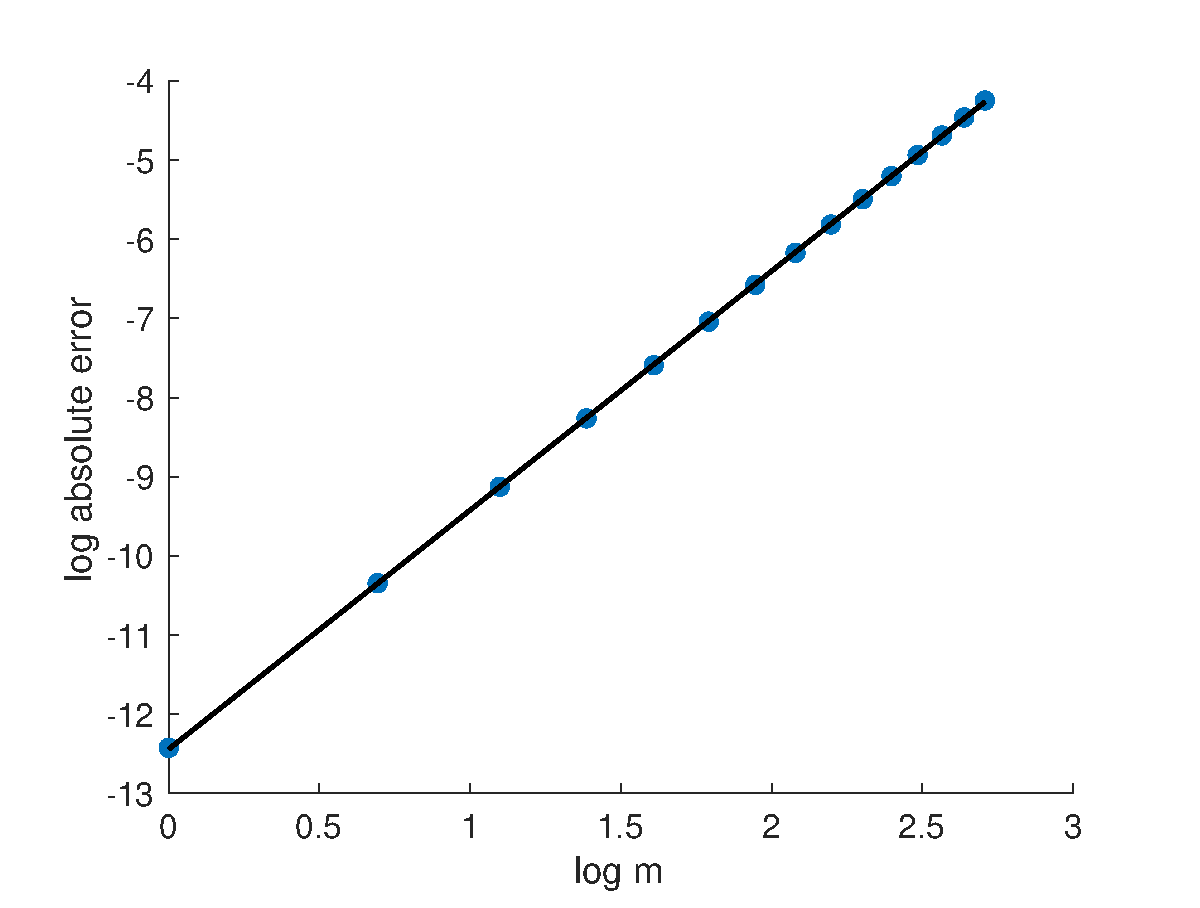
\includegraphics[width=7.5cm]{images/SPesslogerror.eps}
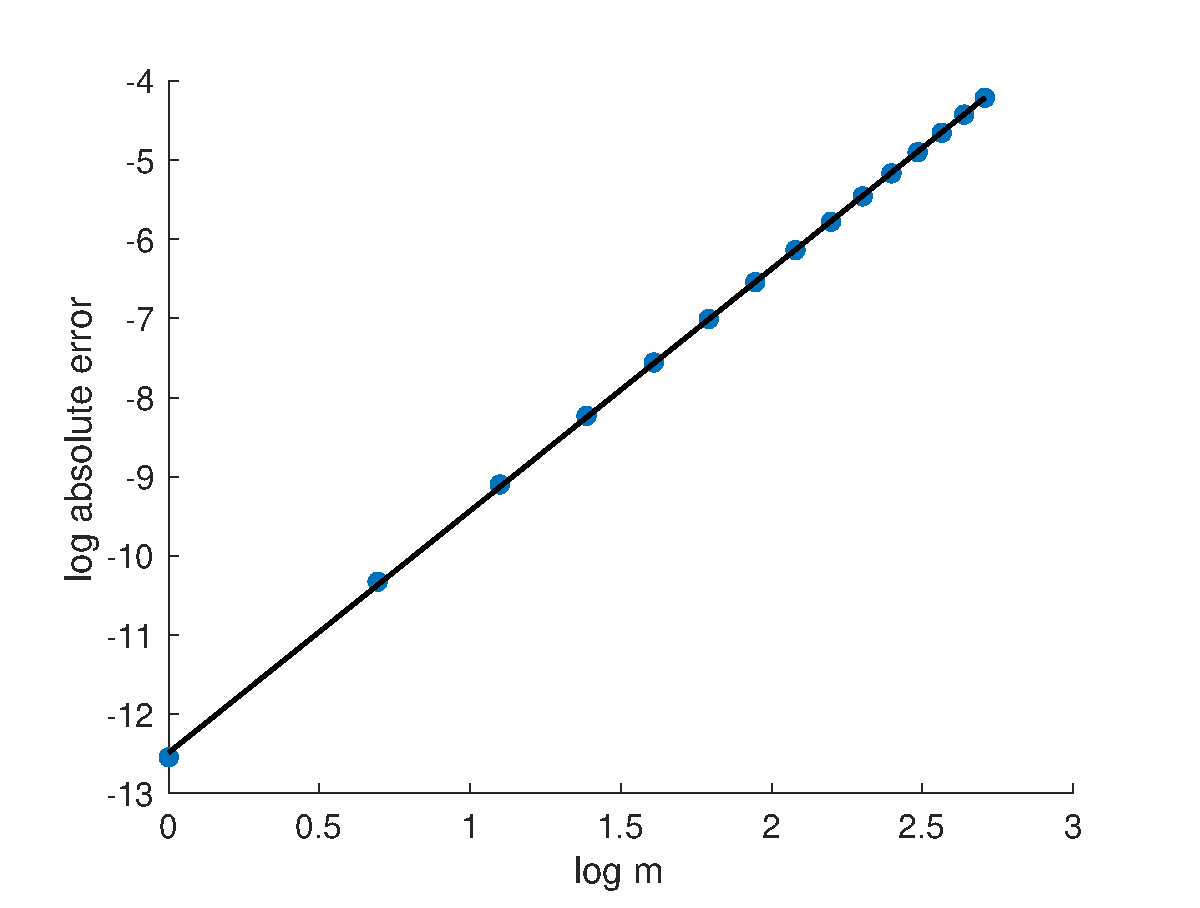
\includegraphics[width=7.5cm]{images/DP2esslogerror.eps} 
\end{tabular}
\end{center}
\caption{Log of absolute error vs. $\log m$ for the first 15 essential spectrum eigenvalues with least squares linear regression line for periodic single pulse (left panel) and second periodic double pulse (right panel). $N = 1024$ grid points, $p = -1$, $c = 10$, $X = 200$.}
\label{fig:DP2esslogerror}
\end{figure}

Finally, we look at what happens when we increase the period $X$. As predicted by \cref{th:Kreinbubble}, there is a brief instability bubble when the first essential spectrum eigenvalue collides with the imaginary interaction eigenvalue (\cref{fig:kreinbubble1}).
\begin{figure}[H]
\begin{center}
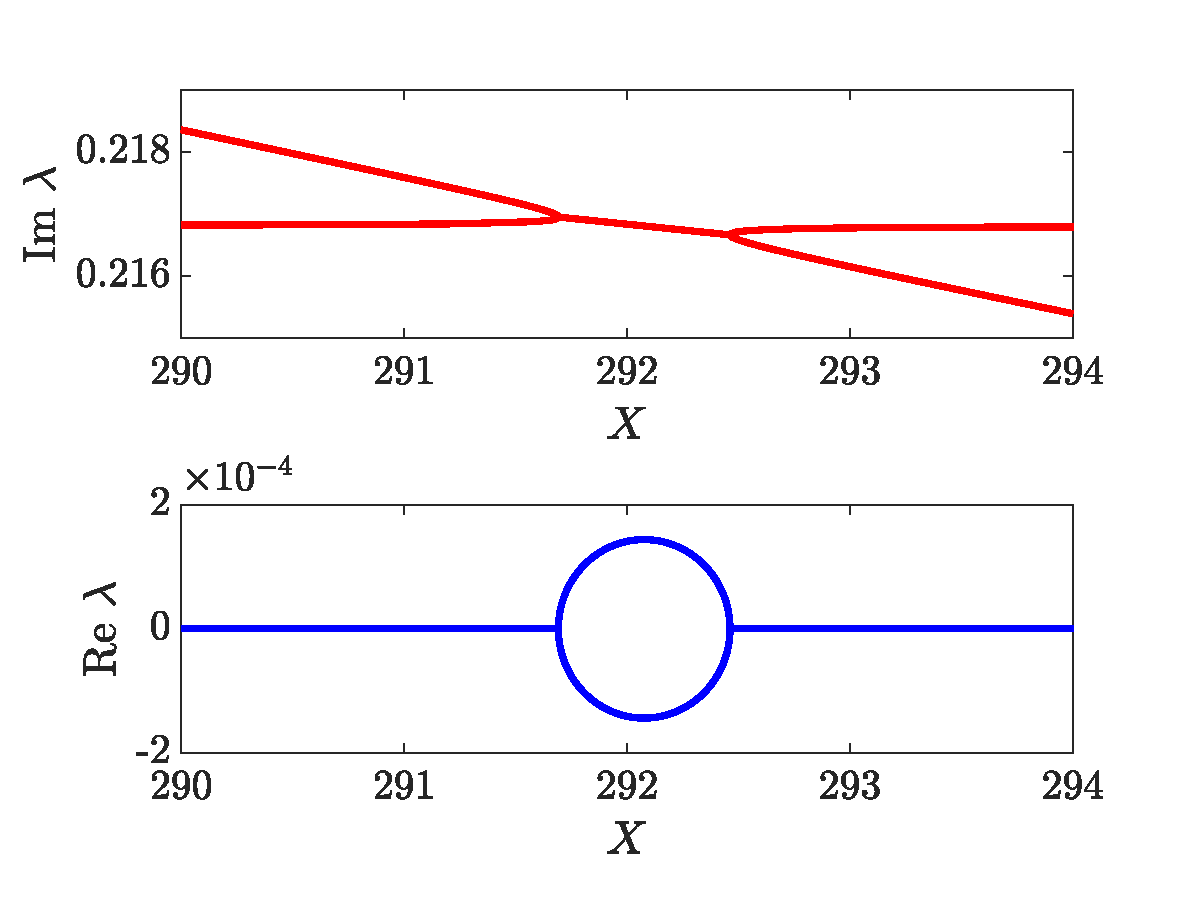
\includegraphics[width=7.5cm]{images/kreinbubble1}
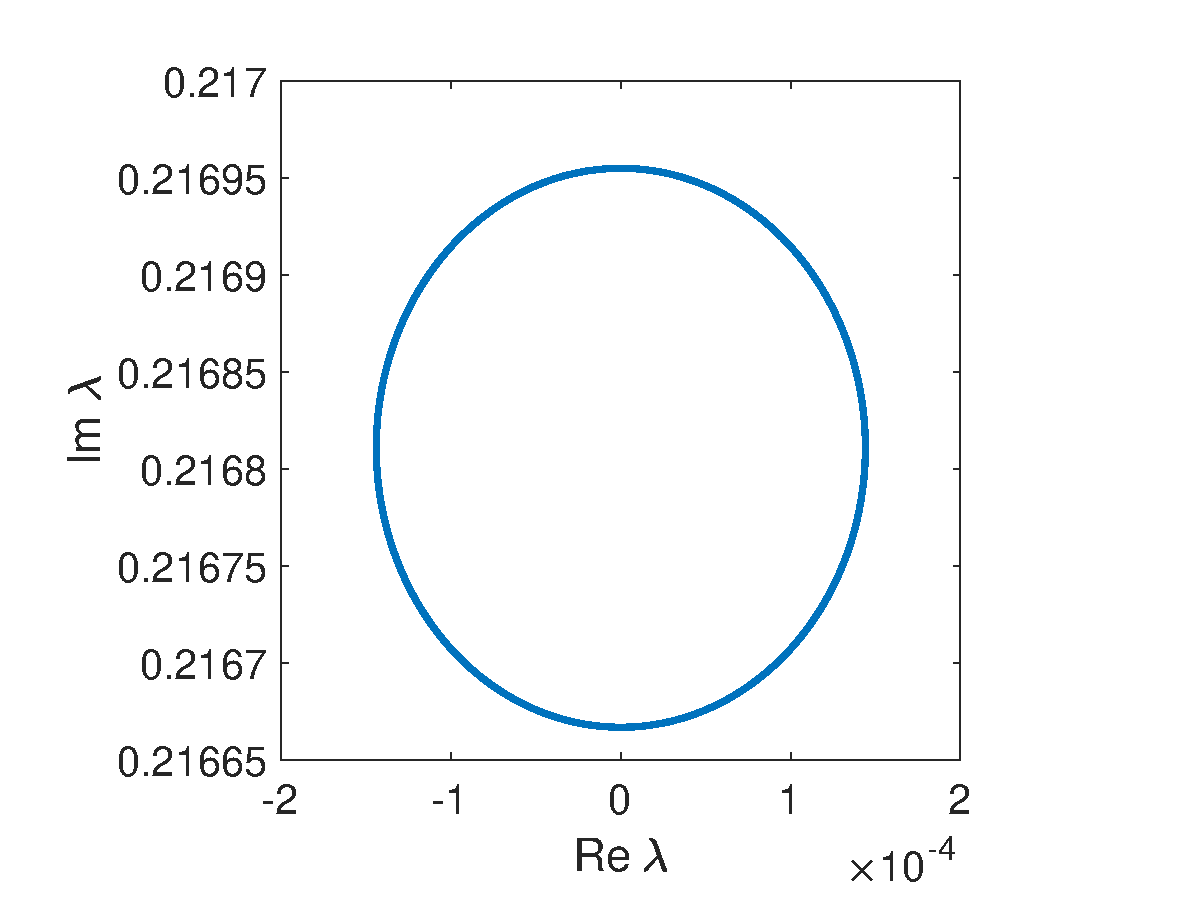
\includegraphics[width=7.5cm]{images/kreinbubble1zoom.eps}
\end{center}
\caption{Left panel shows collision of first essential spectrum eigenvalue with purely imaginary interaction eigenvalue as $X$ is increased. Imaginary part of eigenvalues in top panel (red), real part of eigenvalues in bottom panel (blue). Right panel plots the imaginary part vs. the real part of the eigenvalues in the Krein bubble as $X$ varies. Parameter continuation with AUTO in periodic domain length $X$, $p = -1$, $c = 20$.}
\label{fig:kreinbubble1}
\end{figure}
\noi If $p$ and $c$ in \cref{KdV5eq4} are related by
\begin{align}\label{KdVpabc}
p &= -2(a+b), \quad c = (a+b)^2 && a, b > 0,
\end{align}
then the eigenvalues of $DF(0)$ are the quartet $\pm \sqrt{a} \pm \sqrt{b} i$. Choosing $a = 0.25$ and $b = 3$, so that the tail oscillations of the primary pulse are sufficiently rapid and do not decay too fast, we can construct the first four periodic double pulses with $m_0 = 1$, together with their interaction eigenfunctions, to a sufficient degree of accuracy so that that AUTO converges for both the existence problem and the eigenvalue problem. \cref{fig:kreinerrors} plots the log of the absolute error of the Krein bubble radius in the complex plane and the Krein bubble radius in $X$ ($\Delta X$ from \cref{KreinDeltaX}) versus $\alpha X_0$. 
\begin{figure}[H]
\begin{center}
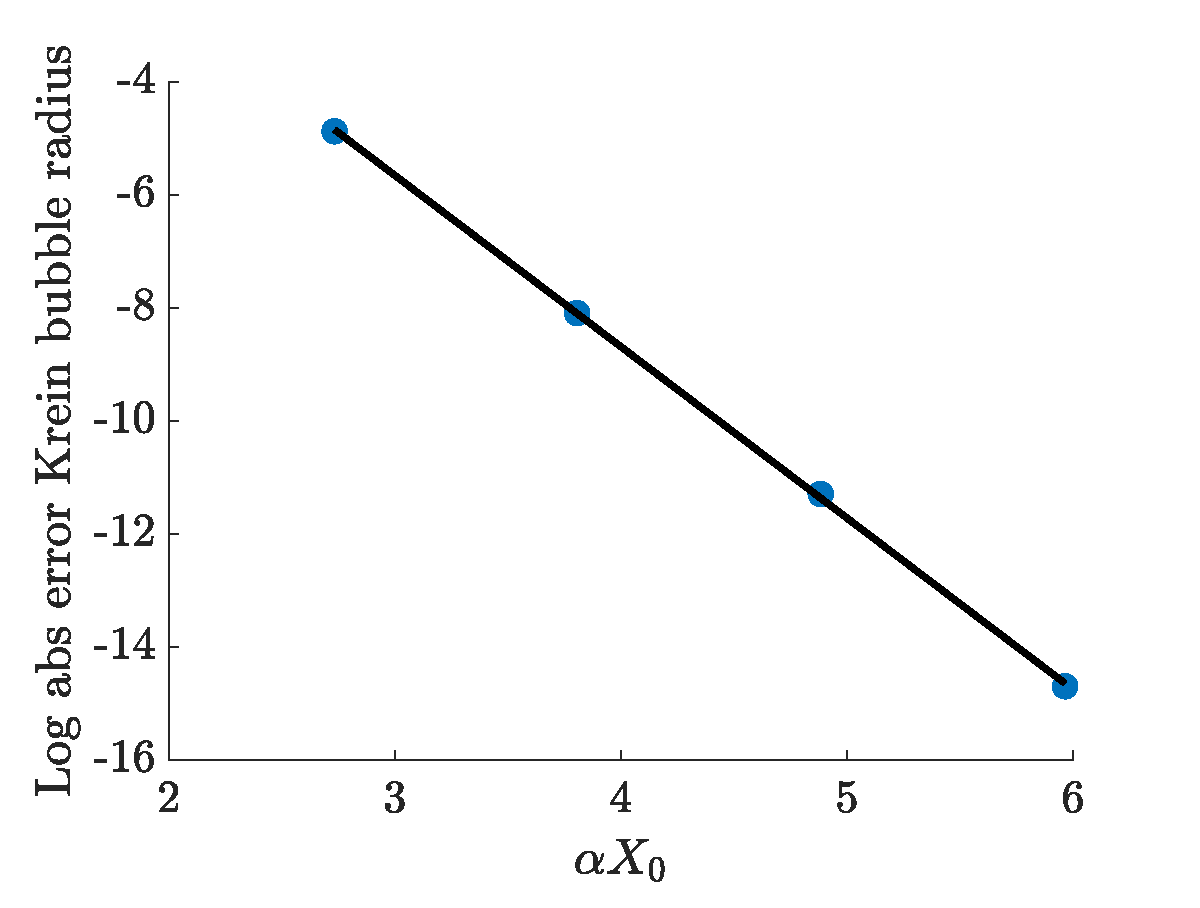
\includegraphics[width=7.5cm]{images/KreinRadiusError.eps}
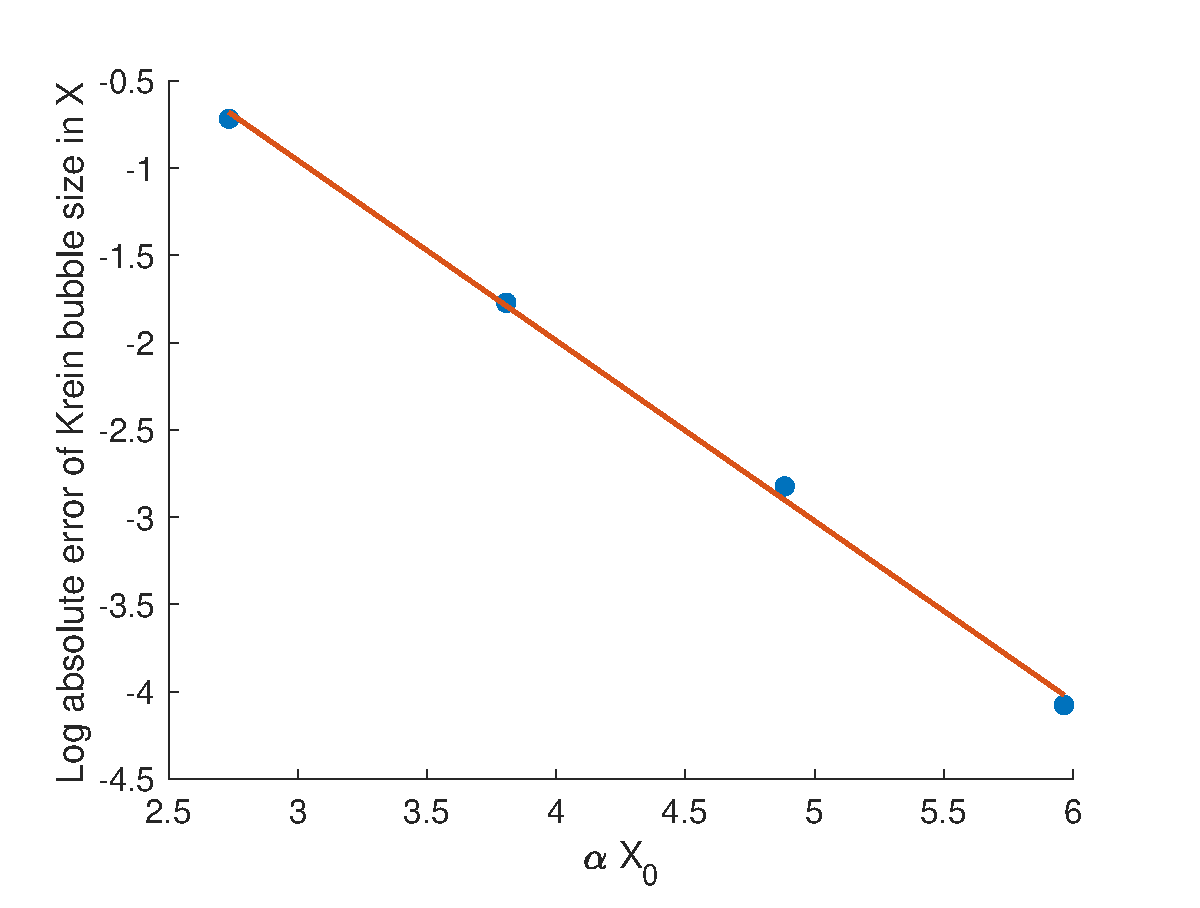
\includegraphics[width=7.5cm]{images/KreinRadiusXError.eps}
\end{center}
\caption{Plot of log of absolute error for Krein bubble radius in the complex plane (left panel) and Krein bubble size in $X$ (right panel) versus $\alpha X_0$ with least-square linear regression lines for first four double pulses with $m_0 = 1$. Parameters $p = 5.3$, $c = 11.2225$.}
\label{fig:kreinerrors}
\end{figure}
\noi The slopes of the least squares linear regression lines suggest that the Krein bubble radius in the complex plane is given by $\sqrt{T_1} + \mathcal{O}(e^{-3 \alpha X_0})$ and that the Krein bubble radius in $X$ is given by $\Delta X + \mathcal{O}(e^{-\alpha X_0})$, with relative errors in the exponent less than 0.01 and 0.03 (respectively). The leading order terms agree with \cref{th:Kreinbubble}, while the error term is higher order than predicted. The results for subsequent Krein bubbles mentioned in \cref{remark:kreinbubbles} can similarly be verified numerically.

\section{Proof of Theorem \ref{transverseint}}\label{sec:transverseintproof}

The proof is similar to that of \cite[Lemma 6.2 and Lemma 6.4]{Kapitula2020}. By \cref{Qexistshyp}, $Q(0; c_0) \neq 0$, $H(Q(0; c_0); c_0) = 0$, and $\nabla_U H(Q(0; c_0); c_0) \neq 0$. By the implicit function theorem, for $c$ close to $c_0$, the 0-level set $H^{-1}(0; c)$ contains a smooth $(2m-1)$-dimensional manifold $K(c)$, with $K(c_0)$ containing $Q(0; c_0)$. The existence result and the smoothness of the map $c \rightarrow Q(x; c)$ follow from the transverse intersection of $\tilde{W}^s(0; c_0)$ and $\tilde{W}^u(0; c_0)$ in $K(c_0) \subset H^{-1}(0; c_0)$, the implicit function theorem, and the smoothness of $F$. Symmetry with respect to the reversor $R$ follows from symmetry of $Q(0; c_0)$ and the symmetry of $H$ from \cref{hyp:H}.

Fix $c \in (c_0 - \delta, c_0 + \delta)$. Since $Q(x; c)$ solves \ref{genODE}, $Q(x; c) \in C^1(\R, \R^{2m})$. By the stable manifold theorem, $Q(x; c)$ is exponentially localized, i.e. for every $\epsilon > 0$ there exists a constant $C$ such that for all $x \in \R$, $|Q(x; c)| \leq C e^{-(\alpha - \epsilon)|x|}$. Substituting $Q(x; c)$ into \cref{genODE} and differentiating with respect to $c$, $\partial_c Q(x; c)$ satisfies
\begin{equation}\label{Qcprime}
[\partial_c Q(x; c)]' = D_U F(Q(x;c); c) \partial_c Q(x; c) - B Q(x;c),
\end{equation}
where $B$ is defined in \cref{defAB}. Define the linear operator $\calL: C^1(\R, \R^{2m}) \rightarrow C^0(\R, \R^{2m})$ by
\begin{equation}\label{defLtv}
\calL = \frac{d}{dx} - D_U F(Q(x;c); c).
\end{equation}
By equation \cref{Qcprime}, $B Q(x;c) \in \ran \calL$ and is exponentially localized. Since $DF(0; c)$ is hyperbolic, it follows from \cite[Lemma~4.2]{Palmer1984} and the roughness theorem for exponential dichotomies \cite{Coppel1978} that $\calL$ is Fredholm with index 0. By \cref{Qexistshyp}, $\ker \calL = \R \partial_x Q'(x; c)$, thus the set of all bounded solutions to \cref{Qcprime} is given by $\{\partial_c Q(x; c) + \R Q'(x; c)\}$.

To show that $\partial_c Q(x; c)$ is exponentially localized, we reformulate equation \cref{Qcprime} in an exponentially weighted space. Choose $\epsilon \in (0,\alpha_0)$ and let $\eta(x)$ be a standard mollifier function \cite[Section~C.5]{Evans2010}. Let
\begin{equation}\label{defQZ}
Q(x; c) = Z(x; c) e^{-(\alpha - \epsilon)r(x)},
\end{equation}
where $r(x) = \eta(x) * |x|$ is smooth, and $r(x) = |x|$ and $r'(x) = 1$ for $|x| > 1$. Substituting \cref{defQZ} into \cref{Qcprime} and simplifying, we obtain the weighted equation
\begin{equation}\label{Zcprime}
[\partial_c Z(x; c)]' = [D_U F(Q(x;c); c) + (\alpha - \epsilon) r'(x) ] Z(x; c) - e^{(\alpha - \epsilon)r(x)} B Q(x;c),
\end{equation}
where the last term on the RHS is bounded. Define the weighted linear operator $\calL_{\alpha - \epsilon}: C^1(\R, \R^{2m}) \rightarrow C^0(\R, \R^{2m})$ by
\begin{equation}\label{defLtvalpha}
\calL_{\alpha - \epsilon} = \frac{d}{dx} - D_U F(Q(x;c); c) - (\alpha - \epsilon) r'(x) \calI.
\end{equation}
Since $B Q(x;c) \in \ran \calL$, $e^{(\alpha - \epsilon)r(x)} B Q(x;c) \in \ran \calL_{\alpha - \epsilon}$. Since $D_U F(0; c)-(\alpha-\epsilon)\calI$ is still hyperbolic with the same unstable dimension as $D_U F(0; c)$, it follows again from \cite[Lemma 4.2]{Palmer1984} that $\calL_{\alpha - \epsilon}$ is Fredholm with index 0. Since $Q'(x; c)$ is exponentially localized by the stable manifold theorem, $e^{(\alpha - \epsilon)r(x)} Q'(x; c)$ is bounded, thus since $Q'(x; c) \in \ker \calL$, $e^{(\alpha - \epsilon)r(x)} Q'(x; c) \in \ker \calL_{\alpha - \epsilon}$. Since any element in $\ker \calL_{\alpha - \epsilon}$ gives an element of $\ker \calL$ via \cref{defQZ}, $\ker \calL_{\alpha - \epsilon} = \R e^{(\alpha - \epsilon)r(x)} Q'(x; c)$. Since $e^{(\alpha - \epsilon)r(x)} B Q(x;c) \in \ran \calL_{\alpha - \epsilon}$, the set of all bounded solutions to \cref{Zcprime} is given by $\{ \partial_c Z(x; c) + \R e^{(\alpha - \epsilon)r(x)} Q'(x;c) \}$, which implies that $\partial_c Q(x; c) = \partial_c Z (x; c) e^{-(\alpha - \epsilon)r(x)}$ is exponentially localized.

\section{Proof of existence results}\label{sec:existproof}

We will construct a periodic $n$-pulse $U(x)$ using Lin's method. For convenience of notation, we will denote the primary pulse by $Q(x)$ instead of $Q_1(x)$. Rather than taking $U(x)$ to be a piecewise perturbation of $Q(x)$, we adapt the technique in \cite{Sandstede1997} and take a piecewise ansatz of the form
\[
U_i^\pm(x) = Q^\pm(x; \beta_i^\pm) + \tilde{Q}_i^\pm(x),
\]
where the functions $Q^\pm(x; \beta_i^\pm)$ parameterize the stable and unstable manifolds $\tilde{W}^s(0)$ and $\tilde{W}^u(0)$ near $Q(0)$, and $\tilde{Q}_i^\pm$ are small remainder functions. In essence, we use the small parameters $\beta_i^\pm$ to break the homoclinic orbit $Q(x)$, and then the remainder functions $\tilde{Q}_i^\pm$ to glue the pieces back together. We will show that we can find a unique piecewise solution $U_i^\pm(x)$ which generically has $n$ jumps in a specified direction. A periodic multi-pulse solution exists if and only if these $n$ jumps are all 0.

\subsection{Setup}

Using \cref{nondegencond}, we decompose the tangent spaces of the stable and unstable manifolds at $Q(0)$ as 
\begin{equation*}
\begin{aligned}
T_{Q(0)}\tilde{W}^u(0) &= \R Q'(0) \oplus Y^- \\
T_{Q(0)}\tilde{W}^s(0) &= \R Q'(0) \oplus Y^+
\end{aligned}
\end{equation*}
The variational and adjoint variational equations associated with \cref{genODE} are
\begin{align}
V' = DF(Q(x)) V \label{vareq1} \\
W' = -DF(Q(x))^* W \label{adjvareq1}.
\end{align}
It follows from \cref{nondegencond} that $Q'(x)$ is the unique bounded solution to \cref{vareq1}, and that there exists a unique bounded solution $\Psi(x)$ to \cref{adjvareq1}. (In both cases, uniqueness is up to scalar multiples). Since we have a conserved quantity $H$, the following lemma gives the exact form of $\Psi(x)$.

\begin{lemma}\label{psiform}
We can take $\Psi(x) = \nabla H(Q(x))$, where $H$ is the conserved quantity from \cref{hyp:H}. In addition, $\Psi(-x) = R \Psi(x)$, where $R$ is the standard reversor operator, and the last component of $\Psi(x)$ is $q'(x)$.
\begin{proof}
Taking the gradient of $\langle F(U; c), \nabla_U H(U; c) \rangle = 0$, $0 = D F(Q(x))^* \nabla H(Q(x)) + D^2 H(Q(x))^* F(Q(x))$. Using standard vector calculus identities, equation \cref{eqODE}, and the fact that the Hessian is self-adjoint,
\begin{align*}
-D F(Q(x))^* \nabla H(Q(x)) &= D^2 H(Q(x)) Q'(x) = \frac{d}{dx} \nabla H(Q(x)),
\end{align*}
thus $\nabla H(Q(x))$ is a solution to \eqref{adjvareq1}. Since $\nabla H$ is continuous and $Q(x)$ is exponentially localized, $\nabla H(Q(x))$ is bounded as well, thus by uniqueness we can take $\Psi(x) = \nabla H(Q(x))$. Using \eqref{genODErev} and the symmetry relation $Q(-x) = R Q(x)$, 
\begin{align*}
[R \Psi(-x)]' = -R DF(Q(-x)) \Psi(-x) 
= -R [-RDF(Q(x))R] \Psi(-x) = DF(Q(x))[ R \Psi(-x) ].
\end{align*}
By uniqueness, $\Psi(x) = R \Psi(-x)$, thus $\Psi(-x) = R \Psi(x)$. By the definition of $F$, if $\Psi(x) = (\psi_1(x), \dots, \psi_{2m}(x))$ is a solution to \cref{adjvareq1}, then $\psi_{2m}(x)$ solves $\calL(q)^* w = [\calE''(q) + c]^* w = 0$. Since $\calL(q)$ is self-adjoint and $\calL(q)q' = 0$, by uniqueness we must have $\psi_{2m}(x) = q'(x)$.
\end{proof}
\end{lemma}

In the next lemma, we collect a few important results about solutions to \cref{vareq1} and \cref{adjvareq1}.

\begin{lemma}\label{eigadjoint}
Consider the linear ODE $V' = A(x)V$ and the corresponding adjoint equation $W' = -A(x)^* W$, where $A(x)$ is a smooth $n \times n$ matrix. Then
\begin{enumerate}[(i)]
\item $\dfrac{d}{dx}\langle V(x), W(x) \rangle = 0$, thus the inner product is constant in $x$.
\item If $W(x)$ is bounded and $V(x) \rightarrow 0$ as $x \rightarrow \infty$ or $x \rightarrow -\infty$, then $\langle V(x), W(x) \rangle = 0$ for all $x \in \R$. The same holds if we reverse the roles of $W$ and $V$.
\item If $\Phi(y, x)$ is the evolution operator for $V'(x) = A(x)V(x)$, then $\Phi(x, y)^*$ is the evolution operator for the adjoint equation $W'(y) = -A(y)^* W(y)$.
\end{enumerate}
\begin{proof}
For part (i), 
\begin{align*}
\dfrac{d}{dx}\langle V(x), W(x) \rangle &= 
\langle V'(x), W(x) \rangle + \langle V(x), W'(x) \rangle \\
&= \langle A(x)V(x), W(x) \rangle + \langle V(x), -A(x)^* W(x) \rangle = 0
\end{align*}
Part (ii) follows from part (i), the Cauchy-Schwartz inequality and the continuity of the norm. For part (iii), take the derivative of the expression $\Phi(y, x)\Phi(x, y) = I$ with respect to $y$ to get
\begin{align*}
0 &= \left(\frac{d}{dy}\Phi(y, x)\right) \Phi(x, y) +
\Phi(y, x)\left(\frac{d}{dy}\Phi(x, y)\right) 
= A(y) + \Phi(y, x)\left(\frac{d}{dy}\Phi(x, y)\right).
\end{align*}
Rearrange and take the transpose of both sides to get
\begin{align*}
\frac{d}{dy}\Phi(x, y)^* &= -A(y)^* \Phi(x, y)^*  
\end{align*}
\end{proof}
\end{lemma}

\noi Using \cref{eigadjoint}(ii), $\Psi(0) \perp \R Q'(0) \oplus Y^+ \oplus Y^-$, thus we can decompose $\R^{2m}$ as
\begin{equation}\label{R2mdecomp}
\R^{2m} = \R Q'(0) \oplus Y^+ \oplus Y^- \oplus \R \Psi(0).
\end{equation}

\subsection{Piecewise ansatz}

First, we write the manifolds $\tilde{W}^u(0)$ and $\tilde{W}^s(0)$ as graphs over their tangent spaces near $Q(0)$. Following \cite{Sandstede1997}, we can parameterize the unstable and stable manifolds near $Q(0)$ by the smooth functions $Q^-(\gamma, \beta^-)$ and $Q^+(\gamma, \beta^+)$, where $\gamma \in \R$, $\beta^\pm \in Y^\pm$. These functions are chosen so that $Q^+(\gamma, 0) - Q^-(\gamma, 0) \in \R \Psi(0)$, and $Q^+(0, 0) = Q^-(0, 0) = Q(0)$. We will always take $\gamma = 0$. Let $Q^\pm(x; \beta^\pm)$ be the unique solutions to \eqref{genODE} on $\R^\pm$ with initial conditions $Q^\pm(0, \beta^\pm)$ at $x = 0$. We will look for a $n-$periodic solution $U(n)$ to \eqref{genODE} which is piecewise of the form
\begin{equation}\label{Upiecewise}
\begin{aligned}
U_i^-(x) &= Q^-(x; \beta_i^-) + \tilde{Q}_i^-(x) && x \in [-X_{i-1}, 0] \\
U_i^+(x) &= Q^+(x; \beta_i^+) + \tilde{Q}_i^+(x) && x \in [0, X_i]
\end{aligned}
\end{equation}
for $i = 0, \dots, n-1$, where $U_i^-: [-X_{i-1}, 0] \rightarrow \R$ and $U_i^+: [0, X_i] \rightarrow \R$ are continuous. The subscripts $i$ are taken $\Mod n$ since we are on a periodic domain, and the pieces are glued together end-to-end as in \cite{Sandstede1998}, with one additional join to ``close the loop''. Since $Q^\pm(0; \beta_i^\pm) \in \R Q'(0) \oplus Y^\pm$, we can choose $\tilde{Q}_i^\pm(x)$ so that
\begin{align*}
\tilde{Q}_i^-(0) &\in \R \Psi(0) \oplus Y^- \\
\tilde{Q}_i^+(0) &\in \R \Psi(0) \oplus Y^+.
\end{align*}
In order to construct a periodic $n$-pulse, we will solve the following system of equations
\begin{align}
(U_i^\pm(x))' - F(U_i^\pm(x)) &= 0 \label{exsystem1} \\
U_i^+(X_i) - U_{i+1}^-(-X_i) &= 0 \label{exsystem2} \\
U_i^+(0) - U_i^-(0) &= 0 \label{exsystem3}
\end{align}
for $i = 0, \dots, n-1$. Equation \cref{exsystem2} is a matching condition at the pulse tails, and equation \cref{exsystem3} is a matching condition at the pulse centers.

\subsection{Exponential Dichotomy}\label{sec:existdichot}

Let $\Phi_\pm(x, y; \beta^\pm)$ be the family of evolution operators for
\begin{align}\label{qpmODEs}
[V^\pm(x)]' &= D F\left(Q^\pm(x, \beta^\pm)\right) V^\pm(x) && x \in \R^\pm.
\end{align}
Choose any $\alpha$ slightly less than $\alpha_0$. In the next lemma, we decompose these evolution operators in exponential dichotomies on $\R^+$ and $\R^-$. 

% lemma : exp dichotomy
\begin{lemma}\label{dichotomy1}
There exist projections
\begin{align*}
&P_+^s(y; \beta^+), \quad P_+^u(y; \beta^+) = I - P_+^s(y; \beta^+) && y \geq 0 \\
&P_-^u(y; \beta^-), \quad P_-^s(y; \beta^-) = I - P_-^u(y; \beta^-) && y \leq 0 
\end{align*}
on $\R^\pm$ such that the evolution operators $\Phi_\pm(x, y; \beta^\pm)$ can be decomposed as
\begin{align*}
\Phi^s_\pm(x, y; \beta^\pm) &= \Phi_\pm(x, y; \beta^\pm) P^s_\pm(y; \beta^\pm) \\
\Phi^u_\pm(x, y; \beta^\pm) &= \Phi_\pm(x, y; \beta^\pm) P^u_\pm(y; \beta^\pm),
\end{align*}
and we have the estimates
\begin{align*}
|\Phi^s_+(x, y, \beta^+)| &\leq C e^{-\alpha(x - y)} && 0 \leq y \leq x \\
|\Phi^u_+(x, y, \beta^+)| &\leq C e^{-\alpha(y - x)} && 0 \leq x \leq y \\
|\Phi^u_-(x, y, \beta^-)| &\leq C e^{-\alpha(y - x)} && 0 \geq y \geq x \\
|\Phi^s_-(x, y, \beta^-)| &\leq C e^{-\alpha(x - y)} && 0 \geq x \geq y,
\end{align*}
which also hold for derivatives with respect to the initial conditions $\beta^\pm$. In addition, the projections satisfy the commuting relations
\begin{align*}
\Phi_\pm(x, y; \beta^\pm) P^{s/u}_\pm(y; \beta^\pm) 
= P^{s/u}_\pm(x; \beta^\pm) \Phi_\pm(x, y; \beta^\pm).
\end{align*}
The projections can be chosen such that at $y = 0$ we have, independent of $\beta^+$ and $\beta^-$
\begin{align*}
\ker P^s_+(0; \beta^+) &= \R \Psi(0) \oplus Y^-, \qquad
\ker P^u_-(0; \beta^-) = \R \Psi(0) \oplus Y^+ \\
\ran P^u_+(0; \beta^+) &= \R \Psi(0) \oplus Y^-, \qquad
\ran P^s_-(0; \beta^-) = \R \Psi(0) \oplus Y^+.
\end{align*}
Let $E_0^s$ and $E_0^u$ be the stable and unstable eigenspaces of $DF(0)$, and let $P_0^s$ and $P_0^u$ be the corresponding eigenprojections. Then we have the following estimates, which are independent of $\beta_i^\pm$.
\begin{equation}\label{projdiffest}
\begin{aligned}
&|P^u_+(x; \beta^+) - P_0^u| \leq C e^{-\alpha x},
&&|P^s_+(x; \beta^+) - P_0^s| \leq C e^{-\alpha x} \\
&|P^u_-(x; \beta^-) - P_0^u| \leq C e^{\alpha x},
&&|P^s_-(x; \beta^-) - P_0^s| \leq C e^{\alpha x} .
\end{aligned}
\end{equation}

\begin{proof}
Since $DF(0)$ is hyperbolic by \cref{hyp:hypeq} and $|\Re \nu| \geq \alpha_0$ for all eigenvalues $\nu$ of $DF(0)$, the exponential dichotomy results follow from \cite[Lemma 5.1]{Sandstede1997}, which follows from \cite[Lemma 1.1]{Sandstede1993}. The estimates \cref{projdiffest} follow from \cite[Lemma 1.1]{Sandstede1993} and \cite[Lemma 2.1]{Sandstede1993}.
\end{proof}
\end{lemma}

\subsection{Fixed Point Formulation}

Next, we formulate equation \eqref{exsystem1} as a fixed point problem. Plug in the piecewise ansatz \eqref{Upiecewise} into \eqref{genODE} and using the fact that $Q^\pm(x; \beta_i^\pm)$ solves \eqref{genODE} on $\R^\pm$,
\begin{align*}
(\tilde{Q}_i^\pm(x))' &= F\left(Q^\pm(x; \beta_i^\pm) + \tilde{Q}_i^\pm(x) \right) - F(Q^\pm(x; \beta_i^\pm)) && i = 0, \dots, n-1
\end{align*}
Expanding the RHS in a Taylor series about $Q^\pm(x; \beta_i^\pm)$, we obtain the ODE for $\tilde{Q}_i^\pm$
\begin{align}\label{Vpiecewise1}
(\tilde{Q}_i^\pm(x))' &= DF(Q^\pm(x; \beta_i^\pm)) \tilde{Q}_i^\pm(x) + G_i^\pm(x; \beta_i^\pm) && i = 0, \dots, n-1
\end{align}
where $G_i^\pm$ depends on $\tilde{Q}_i^\pm$ and
\begin{equation}\label{Gquadratic}
G_i^\pm(x; \beta_i^\pm) = \mathcal{O}(|\tilde{Q}_i^\pm(x)|^2).
\end{equation}
As in \cite{Sandstede1997}, derivatives of $G_i^\pm$ with respect to the parameters $\beta_i^\pm$ are also quadratic in $\tilde{Q}_i^\pm$. We rewrite \eqref{Vpiecewise1} in integrated form to get the fixed point problem
\begin{equation}\label{FPequations}
\begin{aligned}
\tilde{Q}_i^+(x) &= \Phi^u_+(x, X_i; \beta_i^+) a_i^+  
+ \int_{X_i}^x \Phi_+^u(x, y; \beta_i^+) G_i^+(y; \beta_i^+)dy 
+ \int_0^x \Phi_+^s(x, y; \beta_i^+) G_i^+(y; \beta_i^+)dy \\ 
\tilde{Q}_i^-(x) &= \Phi^s_-(x, -X_{i-1}; \beta_i^-) a_{i-1}^-  
+\int_{-X_{i-1}}^x \Phi_-^s(x, y; \beta_i^-) G_i^-(y; \beta_i^-)dy 
+ \int_0^x \Phi_-^u(x, y; \beta_i^-) G_i^-(y; \beta_i^-)dy
\end{aligned}
\end{equation}
where $a_i^+ \in E_0^u$ and $a_i^- \in E_0^s$. Define the exponentially weighted norms
\begin{equation}\label{expwtnorm}
\begin{aligned}
\|V\|_{X, +} &= \sup_{x \in [0, X]} e^{\alpha(X - x)}|V(x)| \\
\|V\|_{X, -} &= \sup_{x \in [-X, 0]} e^{\alpha(X + x)}|V(x)|,
\end{aligned}
\end{equation}
and let $K_{X, \pm}$ be the Banach spaces of continuous functions on $[0, X]$ and $[-X, 0]$ equipped with these norms. Let $B_{X, \pm}(\rho)$ be the ball of radius $\rho$ about $0$ in $K_{X, \pm}$.

\subsection{Inversion}

As in \cite{Sandstede1997}, we will solve for the remainder functions $\tilde{Q}_i^\pm$ and parameters $\beta_i^\pm$ in a series of lemmas. First, we will solve equation \cref{exsystem1} for $\tilde{Q}_i^\pm(x)$.

\begin{lemma}\label{solveforV}
There exist $\delta, \rho > 0$ such that for $|X_i|, |X_{i-1}| > 1/\delta$ and $|a_{i-1}^-|, |a_i^+|, |\beta_i^\pm| < \delta$, there exist unique solutions
\begin{align*}
\tilde{Q}_i^-(a_{i-1}^-, \beta_i^-) &\in B_{X_{i-1}, -}(\rho) \\
\tilde{Q}_i^+(a_i^+, \beta_i^+) &\in B_{X_i, +}(\rho) \\
\end{align*}
to \eqref{FPequations}. $\tilde{Q}_i^-(a_{i-1}, \beta_i^-)$ depends smoothly on $(a_{i-1}^-, \beta_i^-)$, and $\tilde{Q}_i^+(a_i, \beta_i^+)$ depends smoothly on $(a_i^+, \beta_i^+)$, and we have the estimates
\begin{equation}\label{Vest}
\begin{aligned}
\|\tilde{Q}_i^-\|_{X_{i-1}, -} &\leq C |a_{i-1}^-| \\
\|\tilde{Q}_i^+\|_{X_i, +} &\leq C |a_i^+|
\end{aligned}
\end{equation}
where the constant $C$ depends only on $\delta$. The estimates hold for derivatives of $\tilde{Q}_i^\pm$ with respect to $\beta_i^\pm$.
\begin{proof}
The proof follows \cite[Lemma 5.2]{Sandstede1997}. For the first term on the RHS of \eqref{FPequations} on $\R^+$,
\begin{align*}
e^{\alpha(X_i - x)} | \Phi^u_+(x, X_i; \beta_i^+) a_i^+ | 
&\leq C e^{\alpha(X_i - x)} e^{-\alpha(X_i - x)} |a_i^+| = C |a_i^+|,
\end{align*}
and for the second term, since $G_i^+$ is quadratic order in $\tilde{Q}_i^+$ and $\tilde{Q}_i^+ \in K_{X_i, +}$, 
\begin{align*}
e^{\alpha(X_i - x)} &\left| \int_{X_i}^x \Phi_+^u(x, y; \beta_i^+) G_i^+(y; \beta_i^+)dy  \right| 
\leq C e^{\alpha(X_i - x)} \int_x^{X_i} e^{-\alpha(y - x)}|\tilde{Q}_i^+(y)|^2 dy \\
&\leq C e^{\alpha(X_i - x)} \int_x^{X_i} 
e^{-\alpha(y - x)}(e^{-\alpha(X_i - y)})^2|e^{\alpha(X_i - y)} \tilde{Q}_i^+(y)|^2 dy \leq C
\end{align*}
The third term is similarly bounded. Thus the RHS of the fixed point equation \eqref{FPequations} on $\R^+$ is a smooth map $K_{X_i, +} \mapsto K_{X_i, +}$. Define $H: K_{X_i, +} \times E_0^s \times Y^+ \rightarrow K_{X_i, +}$ by
\begin{align*}
H(\tilde{Q}_i^+(x), &a_i^+, \beta_i^+) = \tilde{Q}_i^+(x) - \Phi^u_+(x, X_i; \beta_i^+) a_i^+ - \int_{X_i}^x \Phi_+^u(x, y; \beta_i^+) G_i^+(y; \beta_i^+)dy \\
&- \int_0^x \Phi_+^s(x, y; \beta_i^+) G_i^+(y; \beta_i^+)dy.
\end{align*}
Since $Q(x)$ satisfies \eqref{genODE}, $H(0, 0, 0) = 0$, and since $G_i^+$ is quadratic in $\tilde{Q}_i^+(x)$, the Fr\'echet derivative of $H$ with respect to $\tilde{Q}_i^+(x)$ at $(\tilde{Q}_i^+(x), a_i^+, \beta_i^+) = (0, 0, 0)$ is the identity. Using the implicit function theorem, we can solve for $\tilde{Q}_i^+(x)$ in terms of $(a_i^+, \beta_i^+)$ for sufficiently small $|a_i^+|$ and $|\beta_i^+|$. Since the map $H$ is smooth, this dependence is smooth. The estimate on $\tilde{Q}_i^+$ comes from the first term on the RHS of \eqref{FPequations}, since the remaining terms on the RHS are are quadratic in $\tilde{Q}_i^+$. Since the exponential dichotomy estimates from Lemma \ref{dichotomy1} hold for derivatives with respect to $\beta_i^+$, these do as well. We can similary solve for $\tilde{Q}_i^-$ in terms of $(a_{i-1}^-, \beta_i^-)$.
\end{proof}
\end{lemma}

Next, we will solve equation \cref{exsystem2} to match the pieces \cref{Upiecewise} at $\pm X_i$, which will solve for the initial conditions $a_i^\pm$.

\begin{lemma}\label{solvefora}
For $X_i$ and $\beta_i^\pm$ chosen as in Lemma \ref{solveforV}, there is a unique pair of initial conditions $(a_i^+, a_i^-) \in E_0^s \times E_0^u$ such that $U_i^+(X_i) - U_{i+1}^-(-X_i) = 0$. $(a_i^+, a_i^-)$ depends smoothly on $(\beta_i^+, \beta_{i+1}^-)$, and we have the estimate
\begin{equation}\label{aest}
|a_i^\pm| \leq C e^{-\alpha X_i},
\end{equation}
which holds as well for derivatives with respect to $\beta_i^\pm$. In addition,
\begin{equation}\label{aiformula}
\begin{aligned}
a_i^+ &= -P^u_0 \left( Q^+(X_i; \beta_i^+) - Q^-(-X_i; \beta_{i+1}^-) \right) + \mathcal{O}( e^{-2 \alpha X_i} ) \\
a_i^- &= P^s_0 \left( Q^+(X_i; \beta_i^+) - Q^-(-X_i; \beta_{i+1}^-) \right) + \mathcal{O}\left( e^{-2 \alpha X_i} \right)
\end{aligned}
\end{equation}

\begin{proof}
Evaluating the fixed point equations \cref{FPequations} at $\pm X_i$ and substituting them into \cref{Upiecewise}, the matching condition \cref{exsystem2} becomes $H(a_i^+, a_i^-, \beta_i^+, \beta_{i+1}^-) = 0$, where $H: E_0^s \times E_0^u \times Y^+ \times Y^- \rightarrow \R^{2m}$ is defined by
\begin{align*}
H(a_i^+, &a_i^-, \beta_i^+, \beta_{i+1}^-) 
= a_i^+ - a_i^- + (P^u_+(X_i; \beta_i^+) -  P^u_0)a_i^+ - (P^s_-(-X_i; \beta_{i+1}^-) - P^s_0) a_i^-  \\
&+ Q^+(X_i; \beta_i^+) - Q^-(-X_i; \beta_{i+1}^-)\\
&+ \int_0^{X_i} \Phi_+^s(X_i, y; \beta_i^+) G_i^+(y,\beta_i^+)dy
- \int_0^{-X_i} \Phi_-^u(-X_i, y; \beta_{i+1}^-) G_{i+1}^-(y,\beta_{i+1}^-)dy,
\end{align*}
where we substutited $\tilde{Q}_i^\pm(x)$ from Lemma \ref{solveforV} into $G_i^\pm$. Since $Q(x)$ satisfies \eqref{genODE}, $H(0, 0, 0, 0) = 0$. Since $G_i^\pm$ is quadratic in $\tilde{Q}_i^\pm$, thus quadratic in $a_i^\pm$ by Lemma \ref{solveforV},
\[
\frac{\partial}{\partial a_i^\pm} H(0, 0, 0, 0) = \pm 1 + \mathcal{O} (e^{-\alpha X_i}),
\]
where we also used the estimate \cref{projdiffest}. For sufficiently large $X_i$, $D_{a_i^\pm} H(0, 0, 0, 0)$ is invertible in a neighborhood of $(0, 0, 0, 0)$, thus we can use the implicit function theorem to solve for $a_i^\pm$ in terms of $\beta_i^\pm$. The estimate \cref{aest} then comes from the stable manifold theorem, since $Q^\pm(\pm X_i; \beta_i^\pm) = \mathcal{O}(e^{-\alpha X_i})$. To obtain the expressions \cref{aiformula}, we apply the eigenprojections $P^u_0$ and $P^s_0$ (respectively) to $H(a_i^+, a_i^-, \beta_i^+, \beta_{i+1}^-) = 0$. The bound on the remainder term comes from the bound \cref{aest}, together with the estimates from Lemma \ref{solveforV} and equation \cref{projdiffest}. 
\end{proof}
\end{lemma}

It only remains to solve equation \eqref{exsystem3}, which will match the pieces \eqref{Upiecewise} at $0$. Before we do that, we will use the the flow-box method to make a smooth change of coordinates to ``straighten out'' the stable and unstable manifolds near $Q(0)$ so that their non-intersecting directions are $Y^+$ and $Y^-$.

\begin{lemma}\label{straightenW}
There exists a differentiable map $S: \R \times Y^- \times Y^+ \times \R \Psi(0) \rightarrow \R^{2m}$ such that $S(0, 0, 0, 0) = Q(0)$, $S$ is invertible in a neighborhood of $Q(0)$, and
\begin{align*}
S^{-1}(Q^-(0; \beta^-)) &= \beta^-  \\
S^{-1}(Q^+(0; \beta^+)) &= \beta^+ 
\end{align*}
for sufficiently small $\beta^\pm$.
\begin{proof}
Let $\Theta_x(U_0)$ be the solution operator which maps $U_0 \in \R^{2m}$ to the point $U(x)$, where $U(\cdot)$ is the unique solution to \eqref{genODE} with $U(0) = U_0$. Define the map $S: \R \times Y^- \times Y^+ \times \R \Psi(0) \rightarrow \R^{2m}$ by 
\begin{equation}\label{flowboxdefS}
S(x; \beta^-, \beta^+, \gamma) = \Theta_x\left(Q(0) + Q^-(0; \beta^-) + Q^-(0; \beta^+) + \gamma \Psi(0)\right)
\end{equation}
For small $x$ and $\beta^\pm$ the stable and unstable manifolds are the surfaces
\begin{align*}
\tilde{W}^u &= S(x; \beta^-, 0, 0) \\
\tilde{W}^s &= S(x; 0, \beta^+, 0) 
\end{align*}
Their one-dimensional intersection is the homoclinic orbit $Q(x) = S(x; 0, 0, 0)$, whose tangent space is $Q'(x)$, and $S(0, 0, 0, 0) = Q(0) \neq 0$. The partial derivatives of $S$ are
\begin{align*}
S_x(0, 0, 0, 0) &= F(Q(0)) = Q'(0) \\
S_{\beta^-}(0, 0, 0, 0) &= (Q^-)_{\beta^-}(0; 0) = Y^- \\
S_{\beta^+}(0, 0, 0, 0) &= (Q^+)_{\beta^+}(0; 0) = Y^+ \\
S_{\gamma}(0, 0, 0, 0) &= \Psi(0)
\end{align*}
which span $\R^{2m}$ by \cref{R2mdecomp}. Since the Jacobian of $S$ is invertible at the origin, $S$ is invertible near $Q(0)$ by the inverse function theorem.
\end{proof}
\end{lemma}

Applying this coordinate change near $Q(0)$, the matching condition \cref{exsystem3} is equivalent to projecting $U_i^+(0) - U_i^-(0) = 0$ onto $\R \Q'(0)$, $Y^+$, $Y^-$, and $\R \Psi(0)$ and solving separately on each subspace. Since $P_{\R Q'(0)}(Q^\pm(0; \beta^\pm)) = 0$ and $\tilde{Q}_i^\pm(0) \in \R \Psi(0) \oplus Y^+ \oplus Y^-$, $P_{\R Q'(0)}(U_i^+(0) - U_i^-(0)) = 0$ is automatically satisfied. Since $P_{Y^\pm}(Q^\pm(0; \beta^\pm)) = \beta^\pm$ and $P_{\R \Psi(0)}(Q^\pm(0; \beta^\pm)) = 0$, it remains to solve the equations
\begin{align}
P_{Y^+}(\tilde{Q}_i^+(0) - \tilde{Q}_i^-(0)) + \beta_i^+  &= 0 \label{PY+match} \\
P_{Y^-}(\tilde{Q}_i^+(0) - \tilde{Q}_i^-(0)) - \beta_i^- &= 0 \label{PY-match} \\
P_{\R \Psi(0)}(\tilde{Q}_i^+(0) - \tilde{Q}_i^-(0)) &= 0 \label{PZmatch}
\end{align}
In the next lemma we solve \cref{PY+match} and \cref{PY-match} to obtain the parameters $\beta_i^\pm$.

\begin{lemma}\label{solveforbeta}
For $X_i$ and $\beta_i^\pm$ chosen as in Lemma \ref{solveforV}, and for $i = 0, \dots, n-1$, there exist $(\beta_i^+, \beta_i^-) \in Y^+ \times Y^-$ such that $P_{Y^+ \oplus Y^-}(U_i^+(0) - U_i^-(0)) = 0$. In addition,
\begin{equation}\label{betaest}
\begin{aligned}
|\beta_i^+| &\leq C e^{-2 \alpha X_{i-1}} \\
|\beta_i^-| &\leq C e^{-2 \alpha X_i}
\end{aligned}
\end{equation}
\begin{proof}
Evaluating the fixed point equations \cref{FPequations} at $0$ and substituting them into \cref{Upiecewise}, equations \cref{PY+match} and \cref{PY-match} become $H_i(\beta_i^+, \beta_i^-) = 0$, where $H: Y^+ \oplus Y^- \rightarrow Y^+ \oplus Y^-$ is defined by
\begin{equation}\label{defHPY}
H_i(\beta_i^+, \beta_i^-) = 
\begin{pmatrix}
\beta_i^+ - P_{Y^+}\left(\Phi^s_-(0, -X_{i-1}, \beta_i^-) a_{i-1}^- 
- \int_{-X_{i-1}}^0 \Phi_-^s(0, y, \beta_i^-) G_i^-(y; \beta_i^-) dy\right) \\
\beta_i^- + P_{Y^-}\left( \Phi^u_+(0, X_i; \beta_i^+) a_i^+ 
+ \int_{X_i}^0 \Phi_+^u(0, y; \beta_i^+) G_i^+(y; \beta_i^+)dy \right)
\end{pmatrix},
\end{equation}
and we have substituted our expressions for $\tilde{Q}_i^\pm$ and $a_i^\pm$ from \cref{solveforV} and \cref{solvefora}. Using the estimates from these lemmas together with \cref{dichotomy1},
\begin{equation}\label{DHexp}
D H_i(\beta_i^+, \beta_i^-) = 
\begin{pmatrix}
1 & \mathcal{O}(e^{-2 \alpha X_{i-1}} ) \\
\mathcal{O}(e^{-2 \alpha X_i}) &  1 
\end{pmatrix},
\end{equation}
which is independent of $\beta_i^\pm$, thus $D H_i(\beta_i^+, \beta_i^-)$ is invertible for sufficiently large $X_i$. By the inverse function theorem, $(\beta_i^+, \beta_i^-) = H_i^{-1}(0, 0)$. The estimates \cref{betaest} follow from \cref{defHPY} and Lemmas \ref{dichotomy1}, \ref{solveforV}, and \ref{solvefora}.
\end{proof}
\end{lemma}

We have found a unique solution to \eqref{exsystem1} and \eqref{exsystem2} such that \eqref{exsystem3} is satisfied except for $n$ jumps in the direction of $\Psi(0)$. We summarize what we have obtained so far in the following lemma.

% bounds in this lemma

\begin{lemma}\label{solvewithjumps}
There exists $X^* > 0$ such that for $|X_i| \geq X^*$, $i = 0, \dots, n-1$, there is a unique solution $U(x)$ to equations \eqref{exsystem1}, \eqref{exsystem2}, and \eqref{exsystem3} which is continuous except for $n$ jumps in the direction of $\Psi(0)$. $U(x)$ can be written piecewise in the form 
\begin{equation}\label{Upiecewise2}
\begin{aligned}
U_i^-(x) &= Q^-(x; \beta_i^-) + \tilde{Q}_i^-(x) && x \in [-X_{i-1}, 0] \\
U_i^+(x) &= Q^+(x; \beta_i^+) + \tilde{Q}_i^+(x) && x \in [0, X_i]
\end{aligned}
\end{equation}
where the pieces are glued together end-to-end in a loop. We have the estimates
\begin{enumerate}[(i)]
\item
\begin{equation}\label{tildeQbounds}
\begin{aligned}
|\tilde{Q}_i^-(x)| &\leq C e^{-\alpha(X_{i-1} + x)}e^{-\alpha X_{i-1}} \\
|\tilde{Q}_i^+(x)| &\leq C e^{-\alpha(X_i - x)}e^{-\alpha X_i} 
\end{aligned}
\end{equation}
\item 
\begin{equation}
\begin{aligned}\label{Qpmbounds}
|Q^-(x; \beta_i^-) - Q(x)| &\leq C e^{-2 \alpha X_i} e^{\alpha x} \\
|Q^+(x; \beta_i^+) - Q(x)| &\leq C e^{-2 \alpha X_{i-1}} e^{-\alpha x}
\end{aligned}
\end{equation}
\item
\begin{equation}\label{VQpm}
\begin{aligned}
\tilde{Q}_i^+(X_i) &= Q^-(-X_i; \beta_{i+1}^-) + \mathcal{O}(e^{-2 \alpha X_i}) \\
\tilde{Q}_{i+1}^-(-X_i) &= Q^+(X_i; \beta_i^+) + \mathcal{O}(e^{-2 \alpha X_i})
\end{aligned}
\end{equation}
\end{enumerate}
which hold in addition for derivatives with respect to $x$.
\begin{proof}
Part (i) follows from the estimates \cref{Vest} and \cref{aest} together with the definition of the exponentially weighted norm \cref{expwtnorm}. Part (ii) follows from estimate \eqref{betaest}, smooth dependence on initial conditions, and the stable manifold theorem. For part (iii), in \cref{solvefora} we solved the matching condition at $\pm X_i$
\begin{equation}\label{matchpmXi}
Q^+(X_i; \beta_i^+) + \tilde{Q}_i^+(X_i) = Q^-(-X_i; \beta_{i+1}^-) + \tilde{Q}_i^-(-X_i)
\end{equation}
Applying the projections $P^u_-(-X_i, \beta_{i+1}^-)$ and $P^s_+(X_i, \beta_i^+)$ in turn to \cref{matchpmXi} and using \cref{projdiffest}, the fixed point equations \cref{FPequations}, and the estimates from the previous lemmas in this section, we obtain the estimates \cref{VQpm}.
\end{proof}
\end{lemma}

\subsection{Jump conditions}

Equation \eqref{PZmatch} will give us jump conditions in the direction of the adjoint solution $\Psi(0)$. As in \cite{SandstedeStrut,Sandstede1998} these will only be satisfied for certain values of the lengths $X_i$. 

\begin{lemma}\label{jumplemma1}
A periodic $n$-pulse solution exists if and only if for $i = 0, \dots, n-2$,
\begin{align}\label{jumpcond2}
\xi_i = \langle \Psi(-X_i), Q(X_i) \rangle - \langle \Psi(-X_{i-1}), Q(X_{i-1}) \rangle + R_i = 0
\end{align}
where the remainder term has bound
\begin{align*}
|R_i| \leq C ( e^{-3 \alpha X_i} +  e^{-3 \alpha X_{i-1}})
\end{align*}
\begin{proof}
Evaluating the fixed point equations \eqref{FPequations} at $x = 0$ and substituting them into \eqref{PZmatch},
\begin{equation}\label{PZmatch2}
\begin{aligned}
\langle \Psi(0), &\tilde{Q}_i^+(0) - \tilde{Q}_i^-(0) \rangle = \langle \Psi(0), \Phi^u_+(0, X_i; \beta_i^+) a_i^+ \rangle
- \langle \Psi(0), \Phi^s_-(0, -X_{i-1}, \beta_i^-) a_{i-1}^- \rangle \\
&+ \int_{X_i}^0 \langle \Psi(0), \Phi_+^u(0, y; \beta_i^+) G_i^+(y; \beta_i^+) \rangle dy - \int_{-X_{i-1}}^0 \langle \Psi(0), \Phi_-^s(0, y, \beta_i^-) G_i^-(y; \beta_i^-) \rangle dy
\end{aligned}
\end{equation}
Using Lemma \ref{dichotomy1} together with smooth dependence on initial conditions and the bound \eqref{betaest},
\begin{equation}\label{phibetaest}
\begin{aligned}
|(\Phi_+^u(0, x; \beta_i^+) - \Phi_+^u(0, x; 0)| &\leq C e^{-2 \alpha X_{i-1}} e^{-\alpha x} && x \geq 0\\
|(\Phi_-^s(0, x; \beta_i^-) - \Phi_-^s(0, x; 0)| &\leq C e^{-2 \alpha X_i}e^{\alpha x} &&  x \leq 0\\
\end{aligned}
\end{equation}
To evaluate the term involving $a_i^+$ in \cref{PZmatch2}, we substitute \cref{aiformula} from Lemma \ref{solvefora} for $a_i^+$. Using \eqref{phibetaest}, the estimate \eqref{Qpmbounds}, and Lemma \ref{eigadjoint}(iii),
\begin{align*}
\langle \Psi(0), &\Phi^u_+(0, X_i; \beta_i^+) a_i^+ \rangle = -\langle \Psi(0), \Phi^u_+(0, X_i; \beta_i^+)\left( P^u_0 ( Q^+(X_i; \beta_i^+) - Q^-(-X_i; \beta_{i+1}^-)) + \mathcal{O}( e^{-2 \alpha X_i} ) \right) \rangle \\
&= -\langle \Psi(0), \Phi^u_+(0, X_i; 0) P^u_0 \left( Q^+(X_i; \beta_i^+) - Q^-(-X_i; \beta_{i+1}^-) \right) \rangle + \mathcal{O}( e^{-3 \alpha X_i} + e^{-2\alpha X_{i-1}}e^{-\alpha X_i} ) \\
&= -\langle \Psi(X_i), P^u_+(X_i; 0) P^u_0 \left( Q(X_i) - Q(-X_i) \right) \rangle + \mathcal{O}( e^{-3 \alpha X_i} + e^{-3\alpha X_{i-1}})
\end{align*}
Using \cref{projdiffest}, $P^u_+(X_i; 0) P^u_0 ( Q(X_i) - Q(-X_i)) = Q(-X_i) + \mathcal{O}(e^{-2\alpha X_i})$.
\begin{align*}
\langle \Psi(0), \Phi^u_+(0, X_i; \beta_i^+) a_i^+ \rangle = 
\langle \Psi(X_i), Q(-X_i) \rangle + \mathcal{O}( e^{-3 \alpha X_i} + e^{-3\alpha X_{i-1}})
\end{align*}
Using the reversibility relations $Q(-x) = RQ(x)$ and $\Psi(-x) = R\Psi(x)$ from \cref{varadjsolutions},
\begin{align*}
\langle \Psi(X_i), Q(-X_i) \rangle 
&= \langle R\Psi(-X_i), R Q(X_i) \rangle 
= \langle \Psi(-X_i), Q(X_i) \rangle.
\end{align*}
Combining everything, we obtain equation \cref{jumpcond2} and the remainder bound for $R_i$. By \cite[p. 2093]{SandstedeStrut}, since \cref{eqODE} is a conservative system, if $n-1$ of the jump conditions are satisfied, the final jump condition must automatically be satisfied. Since we are on a periodic domain, it does not matter which condition we eliminate, so choose to eliminate the last one. 
\end{proof}
\end{lemma}

As a corollary, periodic single pulse solutions exist for sufficiently large $X_0$ since for that case there are no jump conditions. These are periodic orbits which are close to the primary homoclinic orbit $Q(x)$.

\begin{corollary}\label{corr:1pexists}
Periodic single pulse solutions exist for sufficiently large $X_0$.
\end{corollary}

\subsection{Rescaling and parameterization}

Following \cite[Section 6]{Sandstede1998}, we will introduce a change of variables with a built-in scaling parameter to facilitate the analysis. Define the set
\begin{align}
\mathcal{R} &= \left\{ \exp\left(-\frac{2 \pi m}{\rho}\right) : m \in \N_0 \right\} \cup \{ 0 \},
\end{align}
where $\rho = \beta_0 / \alpha_0$. Since $\mathcal{R}$ is closed and bounded, it is compact, thus complete. For $r \in \mathcal{R}$, let
\begin{equation}\label{Xstar}
X^* = -\frac{1}{2\alpha_0}\log r - \frac{\phi}{2\beta_0}
\end{equation}
so that
\begin{equation}\label{defr}
r = e^{-\alpha_0(2X^* + \phi/\beta_0)}
\end{equation}
We will use $r$ as a scaling parameter for the system. For $i = 0, \dots n-1$, let
\begin{equation}\label{bjscale}
b_i = e^{-2 \alpha_0 (X_i - X^*)},
\end{equation}
where $X_i \geq X^*$ for $i = 0, \dots, n-1$. The quantities $b_i$ are length parameters for the system. In terms of $r$ and $b_i$,
\begin{equation}\label{Xiscale}
X_i = -\frac{1}{2\alpha_0}\log(b_i r) - \frac{\phi}{2 \beta_0}
\end{equation}
In the next lemma, we rewrite the system \eqref{jumpcond2} using this rescaling.

\begin{lemma}\label{jumplemma3}
A periodic multi-pulse solution exists if and only if for $i = 0, \dots, n-2$
\begin{equation}\label{Geq}
G_i(b_1, \dots, b_{n-1}, r) = b_i \sin \left( -\rho \log b_i \right) - b_{n-1} \sin \left( -\rho \log b_{n-1} \right) + \mathcal{O}(r^{\gamma / 2 \alpha}) = 0
\end{equation}
where $r \in \mathcal{R}$. All derivatives of the remainder term with respect to $b_i$ are also $\mathcal{O}(r^{\gamma / 2 \alpha})$. 
\begin{proof}
Using \cite[Lemma 6.1(i)]{Sandstede1998}, for $x > 0$ sufficiently large,
\begin{equation}\label{IPalphabeta}
\langle \Psi(-x), Q(x) \rangle
= p_0 e^{-2 \alpha_0 x} \sin(2 \beta_0 x + \phi) + \mathcal{O}(e^{-(2 \alpha_0 + \gamma) x})
\end{equation}
where $0 < \gamma \leq 1$, $p_0 > 0$, and $\phi$ are constants. We do not have a parameter $\mu$ in this system, so the $\mu$-dependent terms in \cite[Lemma 6.1(i)]{Sandstede1998} are constant and $\beta(\mu) = \beta_0$. We will always take $\gamma \leq 1$. Substituting \cref{IPalphabeta} into \cref{jumpcond2} and rescaling using \cref{Xiscale} and \cref{bjscale},
\begin{align}\label{diff2}
\langle \Psi(-x), Q(x) \rangle = p_0 e^{\alpha \phi / \beta_0 } b_i r \sin \left( - \rho \log (b_i r) \right) - p_0 e^{\alpha \phi / \beta_0 } b_{i-1} r \sin \left( -\rho \log (b_{i-1} r) \right) + \mathcal{O}(r^{1 + \gamma / 2 \alpha}) &= 0.
\end{align}
Dividing both sides by $r > 0$ and $p_0 e^{\alpha \phi / \beta_0 } > 0$ and simplifying, we obtain the jump conditions
\begin{align}\label{diff3}
\xi_i = b_i \sin \left( -\rho \log b_i \right) - b_{i-1} \sin \left( -\rho \log b_{i-1} \right) + \mathcal{O}(r^{\gamma / 2 \alpha}) &= 0,
\end{align} 
where we used the fact that $\sin \left( -\rho \log (b_i r) \right) = \sin \left( -\rho \log b_i \right)$ for $r \in \mathcal{R}$. For $i = 0, \dots, n-2$, let
\begin{equation}\label{Gidef}
G_i(b_1, \dots, b_{n-1}, r) = \sum_{k = 0}^i \xi_k
\end{equation}
After canceling terms, we obtain the equations \cref{Geq}, which are equivalent to \cref{jumpcond2} since they are a linear combination of the jumps $\xi_i$.
\end{proof}
\end{lemma}

\begin{remark}
In \cref{jumplemma3}, we rewrote \cref{jumpcond2} so that equation $i$ inolves $b_i$ and a common parameter $b_{n-1}$. Since we are on a periodic domain, that choice was arbitrary;  the final length parameter $b_{n-1}$ was chosen for notational convenience.
\end{remark}

When $r = 0$, the equations \eqref{Geq} all have the same form. Let
\begin{equation}\label{defH}
H(b_0, b_1) = b_0 \sin \left( -\rho \log b_0 \right) - b_1 \sin \left( -\rho \log b_1 \right)
\end{equation}
In the next lemma, we will show that pitchfork bifurcations occur on the diagonal in the zero set of $H(b_0, b_1)$.

% lemma: pitchforks
\begin{lemma}\label{pitchforkH}
A discrete family of pitchfork bifurcations occurs along the diagonal in the zero set of $H(b_0, b_1)$ at $(b_0, b_1) = (b_k^*, b_k^*)$ for $k \in \Z$, where
\begin{align}\label{pkstar}
b^*_k = e^{-\frac{1}{\rho} (p^* + k \pi) }, \quad p^* = \arctan \rho 
\end{align}
Locally, the arms of the pitchfork bifurcations open upwards along the diagonal.
\begin{proof}
First, we note that the partial derivative $H_{b_0}(b_0, b_1) = 0$ if and only if $b_0 = b_k^*$ for integer $k$, which gives the locations of the bifurcation points. Next, we change coordinates so that the pitchfork bifurcation will occur along the horizontal axis. Let $b_0 = y-x$ and $b_1 = y+x$, which is a rotation by $-\pi/4$. Making this substitution yields
\begin{equation}\label{Hxy}
H(x, y) = 
(y - x) \sin \left( -\rho \log(y - x) \right) - (y + x) \sin \left( - \rho \log (y + x) \right)
\end{equation}
For all $y$, $H(-x, y) = -H(x, y)$, which is the required odd symmetry for a pitchfork bifurcation. Let $(x_0, y_0) = \left(0, b^*_k \right)$. Evaluating the relevant partial derivatives of $H$ at $(x_0, y_0)$,
\begin{align*}
H_x(x_0, y_0) &= 0, \quad H_y(x_0, y_0) = 0, \quad H_{xx}(x_0, y_0) = 0, \quad H_{yy}(x_0, y_0) = 0 \\
H_{xy}(x_0, y_0) &= (-1)^k 2 \rho \sqrt{1 + \rho^2} \: \exp{\left(\frac{1}{\rho} (\arctan \rho - k \pi) \right)} \neq 0 \\
H_{xxx}(x_0, y_0)
&= -(-1)^k 2 \rho \sqrt{1 + \rho^2} \: \exp{\left(\frac{2}{\rho} (\arctan \rho - k \pi) \right)} \neq 0,
\end{align*}
thus a pitchfork bifurcation occurs at $(0, b^*_k)$ for all $k \in \Z$. To leading order, near the bifurcation points $(0, b_k^*)$, the arms of the pitchforks are upwards-opening parabolas of the form $y = b_k^* + c_k x^2$, where
\begin{equation*}
c_k = \frac{1}{6}\exp{\left(\frac{1}{\rho} (\arctan \rho - k \pi) \right)} > 0
\end{equation*}
The result follows upon returning to the $(b_0, b_1)$ coordinate system.
\end{proof}
\end{lemma}

Now that we have located the pitchfork bifurcations, we will construct a natural parameterization for the zero set of $H(b_0, b_1)$. We only need to consider $b_0 \geq b_1$ since the zero set is symmetric across the diagonal. For any nonnegative integers $m_1 \geq m_0$, the point
\[
(b_0, b_1) = \left( e^{\frac{-m_0 \pi}{\rho}}, e^{\frac{-m_1 \pi}{\rho}}\right)
\]
is in the zero set of $H$. We will use these points to anchor our parameterization, and will use a phase parameter $\theta$ to connect these anchor points. 

\begin{lemma}\label{thetaparamlemma}
For any nonnegative integers $m_0$, $m_1$ with $m_1 \geq m_0$, there is a smooth family of solutions
\begin{align*}
\left( b_0( m_0, m_1, \theta), b_1( m_0, m_1, \theta) \right) && \theta \in [-\pi + p^*, p^*]
\end{align*}
to $H(b_0, b_1) = 0$. This parameterization is given explicitly by
\begin{equation}\label{thetaparam}
\begin{aligned}
b_0( m_0, m_1, \theta) = \exp\left( -\frac{1}{\rho}(m_0 \pi + \theta^*(\theta, m_1 - m_0) \right), \quad
b_1( m_0, m_1, \theta) = \exp\left( -\frac{1}{\rho}(m_1 \pi + \theta) \right),
\end{aligned}
\end{equation}
where $\theta^*(\theta, m) : [-\pi + p^*, p^*] \rightarrow \R$ is smooth in $\theta$ for all $m$ and has the following properties.
\begin{enumerate}[(i)]
\item $\theta^*(\theta; 0) = \theta $
\item $\theta^*(0; m) = 0 \text{ for all } m$
\item $|\theta^*(\theta; m)| \leq |\theta|$
\item $\theta^*(p^*; m) = \theta^*(-\pi+p^*; m+1)$
\item $|\theta^*(\theta; m)| \leq C \exp\left(-\frac{m \pi}{\rho} \right)$
\end{enumerate}
In particular, $\theta^*(p^*, 0) = \theta^*(\pi - p^*, 1) = p^*$.
\begin{proof}
The proof is routine computation. Let $I = [-\pi + p^*, p^*]$. We will substitute the ansatz 
\begin{equation}\label{thetaansatz}
\begin{aligned}
b_0( m_0, m_1, \theta) &= \exp\left(-\frac{1}{\rho}(m_0 \pi + \theta^*) \right), \quad
b_1( m_0, m_1, \theta) &= \exp\left(-\frac{1}{\rho}(m_1 \pi + \theta) \right)
\end{aligned}
\end{equation}
into $H(b_0, b_1) = 0$ and then solve for $\theta^*$ in terms of $\theta$.
\begin{enumerate}
\item First, we show that $\theta^*$ only depends on the difference $m_1 - m_0$. Substituting \cref{thetaansatz} into $H(b_0, b_1) = 0$ and simplifying,
\begin{align*}
e^{-\frac{1}{\rho}m_0 \pi} (-1)^{m_0} \left( e^{-\frac{1}{\rho}\theta^*}\sin \theta^* - e^{-\frac{1}{\rho}(m_1 - m_0) \pi} (-1)^{m_1 - m_0} e^{-\frac{1}{\rho}\theta}\sin \theta \right) = 0.
\end{align*}
Dividing by $e^{-\frac{1}{\rho}m_0 \pi} (-1)^{m_0}$ yields
\begin{equation}\label{thetaeq1}
e^{-\frac{1}{\rho}\theta^*}\sin \theta^* = e^{-\frac{1}{\rho}(m_1 - m_0) \pi} (-1)^{m_1 - m_0} e^{-\frac{1}{\rho}\theta}\sin \theta = 0,
\end{equation}
which only depends on the difference $m_1 - m_0$. Letting $m = m_1 - m_0$, it suffices to solve
\begin{equation}\label{thetaeq2}
g(\theta^*) = t(m) g(\theta)
\end{equation}
for all nonnegative integers $m$, where
\begin{align*}
g(\theta) = e^{-\frac{1}{\rho}\theta}\sin \theta, \quad t(m) = (-1)^m e^{-\frac{1}{\rho}m \pi} 
\end{align*}

\item For $m = 0$, $t(0) = 1$, thus $\theta^*(\theta, 0) = \theta$.

\item For $m \geq 1$, we first show that $g(\theta)$ is invertible on $I$. Since
\begin{equation}\label{gprime}
g'(\theta) = e^{ -\frac{1}{\rho} \theta } \left( \cos \theta - \frac{1}{\rho} \sin \theta \right),
\end{equation}
$g'(p^*) = 0$, $g'(-\pi+p^*) = 0$, and the only only critical point of $g'(\theta)$ on $I$ is a local maximum at $\theta = - \pi + 2 p^*$, $g(\theta)$ is strictly increasing, thus invertible, on $I$. Let
\begin{equation}\label{grange}
g(I) = [-e^{\frac{1}{\rho}\pi} T, T], \quad T = e^{-\frac{1}{\rho}p^*} \sin p^* = \frac{\rho}{\sqrt{1+\rho^2}}e^{-\frac{1}{\rho}\arctan \rho}.
\end{equation}
Then $g: I \rightarrow g(I)$ is a bijection and $g^{-1}: g(I) \rightarrow I$ is also strictly increasing. Since the only zero of $g(\theta)$ on $I$ occurs at $\theta = 0$, $g^{-1}(0) = 0$. We can now solve $g(\theta^*) = t(m) g(\theta)$. For all $\theta \in I$,
\begin{equation}\label{RHSbounds}
	t(m)g(\theta) \in
	\begin{cases}
	[-e^{-\frac{1}{\rho}(m-1) \pi} T, e^{-\frac{1}{\rho}m \pi} T] & m \text{ even }\\
	[-e^{-\frac{1}{\rho}m \pi} T, e^{-\frac{1}{\rho}(m-1) \pi} T] & m \text{ odd }
	\end{cases}.
\end{equation}
Since $t(m)g(\theta) \subset g(I)$ for all $\theta \in I$, we define
\begin{align}\label{solvethetastar}
\theta^*(\theta, m) &= g^{-1}\left( t(m) g(\theta) \right) && \theta \in I, m \geq 1
\end{align}
Since $g(0) = 0$, $\theta^*(0, m) = 0$ for all $m$.

\item Next, we show that $|\theta^*(\theta, m)| \leq |\theta|$. For $m = 0$, we have equality. For $m = 1$ and $\theta = -\pi + p^*$, $t(-\pi + p^*)g(-\pi + p^*) = T$, thus $\theta^*(-\pi + p^*, 1) = -\pi + p^*$. For any other $m$ and $\theta$, it follows from \cref{RHSbounds} that $t(m)g(\theta) \in [e^{-\frac{1}{\rho}\pi}T, T)$, which is strictly contained in $G(I)$. Since $g^{-1}$ is strictly increasing and $g(0) = 0$, $|\theta^*(\theta, m) \leq |\theta|$.

\item We now show that the parameterizations match up at the endpoints. For $m \geq 0$, 
\begin{align*}
\theta^*(p^*, m) &= g^{-1}\left( e^{-\frac{1}{\rho}m \pi} (-1)^m e^{-\frac{1}{\rho}p^*} \sin p^* \right)
\end{align*}
and
\begin{align*}
\theta^*(-\pi + p^*, m+1) &= g^{-1}\left( e^{-\frac{1}{\rho}(m+1) \pi} (-1)^{m+1} e^{-\frac{1}{\rho}(-\pi + p^*)} \sin (-\pi + p^*) \right) \\
&=g^{-1}\left( e^{-\frac{1}{\rho}m \pi} (-1)^m e^{-\frac{1}{\rho}p^*} \sin p^* \right)
\end{align*}
which are equal. In particular, $\theta^*(p^*, 0) = \theta^*(\pi - p^*, 1) = p^*$.

\item Finally, we obtain a bound on $\theta^*(\theta, m)$. For $m \geq 2$ and $\theta \in I$, it follows from \cref{RHSbounds} that $t(m)g(\theta) \in \tilde{I}$, which is strictly contained in $I$. Since $g'(0) = 0$ only at the endpoints of $I$ and is positive in the interior of $I$, $g'(\theta)$ is bounded below on $\tilde{I}$, thus $[g^{-1}]'(\theta)$ is bounded for $\theta \in g(\tilde{I})$. Since $|t(m)g(\theta)| \leq e^{-\frac{1}{\rho}(m - 1)\pi}T$ by \cref{RHSbounds} and $g(0) = 0$, we have the bound (v), which is independent of $\theta$.
\end{enumerate}
\end{proof}
\end{lemma}

\subsection{Proof of Theorem \ref{th:perexist}}

By \cref{jumplemma3}, a periodic $n$-pulse exists if and only if $G_i(b_0, \dots, b_{n-1}, r) = 0$ for $i = 0, \dots, n-2$. When $r = 0$, $G_i(b_0, \dots, b_{n-1}, 0) = H(b_i, b_{n-1})$, and we can use the parameterization from \cref{thetaparamlemma}. Choose any periodic parameterization according to \cref{def:perparam}. Using \cref{thetaparamlemma}, let
\begin{equation}\label{thetaparammulti}
\begin{aligned}
b_i( m_i, m_{n-1}, \theta) &= \exp\left( -\frac{1}{\rho}(m_i \pi + \theta^*(\theta, m_{n-1} - m_i) \right) && i = 0, \dots, n-2 \\
b_{n-1}( m_{n-1}, \theta) &= \exp\left( -\frac{1}{\rho}(m_{n-1} \pi + \theta) \right) \\
b^* &= (b_0( m_0, m_{n-1}, \theta), \dots, b_{n-2}( m_{n-2}, m_{n-1}, \theta) ) \in \R^{n-1}
\end{aligned}
\end{equation}
so that
\begin{align*}
H(b_i( m_i, m_{n-1}, \theta), b_{n-1}( m_{n-1}, \theta) ) &= 0 && i = 0, \dots, n-2
\end{align*}
Substituting $b_{n-1}(m_{n-1}, \theta)$ for $b_{n-1}$ in \eqref{Geq}, define $G: \R^{n-1} \times \mathcal{R} \rightarrow \R^{n-1}$ by $G = (G_0, \dots, G_{n-2})^T$, where 
\begin{equation*}
G_i(b, r) = b_i \sin \left( -\rho \log b_i \right) - b_{n-1}(m_{n-1}, \theta) \sin \left( -\rho \log b_{n-1}(m_{n-1}, \theta) \right) + \mathcal{O}(r^{\gamma / 2 \alpha})
\end{equation*}
and $b = (b_0, \dots, b_{n-1})$. $G(b^*, 0) = 0$, and the Jacobian matrix $D_b G(b^*,0)$ is diagonal, with
\begin{align*}
\partial_{b_i} G_i(b^*, 0)
&= \sin \left( -\rho \log b_i(m_i, \theta) \right) - \rho \cos \left( -\rho \log b_i(m_i, \theta) \right)
\end{align*}
From Lemma \ref{pitchforkH}, $\partial_{b_i} G_i(b, 0) = 0$ if and only if $b_i$ is one of the pitchfork bifurcation points $b_k^*$. By \cref{thetaparamlemma}, if we exclude $\theta \in \{ -\pi + p^*, p^* \}$, the Jacobian $D_b G(b^*,0)$ is invertible, and we can use the implicit function theorem to solve for $b$ in terms of $r$ near $b^*$. Specifically, there exists $r_* > 0$ and a continuous function $b: \mathcal{R} \cap [0, r_*] \rightarrow \R^{n-1}$ given by $b(r) = \left( b_0(r), \dots, b_{n-2}(r) \right)$ such that $b(0) = b^*$ and $G(b(r),r) = 0$. For $i = 0, \dots, n-2$, define $t_i(r; m_i, \theta): \mathcal{R} \rightarrow \R$ by
\begin{equation}\label{defti}
t_i(r; m_i, m_{n-1}, \theta) = -\rho \log b_i(r)
\end{equation}
The functions $t_i(r; m_i, m_{n-1}, \theta)$ are continuous in $r$, and from \cref{thetaparammulti} we have $t_i(0; m_i, m_{n-1}, \theta) = m_i \pi + \theta^*(\theta, m_{n-1} - m_i)$. Equations \cref{Xi} are obtained by substituting $b_i(r)$, $i = 0, \dots, n-2$, and $b_{n-1}(m_{n-1}, \theta)$ for $b_i$ in \cref{Xiscale} and using \cref{defti}.

\subsection{Periodic 2-pulse}

For the periodic 2-pulse, we have a single jump condition
\begin{equation}\label{2pulsedefG}
G(b_0, b_1, r) = b_0 \sin \left( -\rho \log b_0 \right) - b_1 \sin \left( -\rho \log b_1 \right) + \mathcal{O}(r^{\gamma / 2 \alpha}) = 0 \\
\end{equation}

First, we will show that that the pitchfork bifurcations along the diagonal persist for small $r$. Recall that by \cref{def:perparam}, $m_0 \in \{0, 1\}$ for a periodic 2-pulse.

\begin{lemma}\label{pitchpersist}
There exists $r_2 > 0$ such that for $m_0 \in \{0, 1\}$ and $r \leq r_2$, there is a non-degenerate pitchfork bifurcation in the zero set of $G(b_0, b_1, r)$ at $(b_{m_0}^*(r),b_{m_0}^*(r))$, and 
\begin{equation*}
b_{m_0}^*(r) \rightarrow b_{m_0}^* \text{ as } r \rightarrow 0
\end{equation*}
\begin{proof}
Take $m_0 = 0$. The proof is identical for $m_0 = 1$. First, we show the required odd symmetry relation. By Lemma \ref{solvewithjumps}, for an ordered pair $(X_0, X_1)$ with $X_i$ sufficiently large, there exists a unique piecewise solution $(U_0^-(x), U_0^+(x), U_1^-(x), U_1^+(x))$ which is continuous except for two jumps 
\begin{equation}\label{xijumps}
\xi_0(X_0, X_1) = \langle \Psi(0), U_0^+(0) - U_0^-(0) \rangle, \quad
\xi_1(X_0, X_1) = \langle \Psi(0), U_1^+(0) - U_1^-(0) \rangle 
\end{equation}
in the direction of $\Psi(0)$. By symmetry, $(U_1^+(-x), U_1^-(-x), U_0^+(-x), U_0^-(-x))$ is also a solution for $(X_0, X_1)$, thus it must be the same solution by uniqueness. In particular, $U_1^+(0) = U_0^-(0)$ and $U_1^-(0) = U_0^+(0)$, thus $\xi_0(X_0, X_1) = -\xi_1(X_0, X_1) = -\xi_0(X_1, X_0)$. Since swapping $X_0$ and $X_1$ is equivalent to swapping $b_0$ and $b_1$ in \cref{2pulsedefG}, $G(b_0, b_1, r) = -G(b_1, b_0, r)$ for sufficiently small $r$. Making the change of coordinates $(b_0, b_1) \mapsto (x, y)$ as in Lemma \ref{pitchforkH}, $G(-x, y, r) = -G(x, y, r)$ for sufficiently small $r$. 

The persistence of the pitchfork bifurcation follows from a Lyapunov-Schmidt reduction.  By Lemma \ref{pitchforkH}, $G_x(0, b_0^*, 0) = 0$ and $G_{xy}(0, b_0^*, 0) \neq 0$, thus by the implicit function theorem there exists $r_2 > 0$, an open interval $(-a, a)$, and a unique smooth function $y = y^*(x, r)$ such that $y^*(0, 0) = b_0^*$ and $G_x(x, y^*(x, r), r) = 0$ for all $x \in (-a, a)$ and $r < r_2$. It follows that a pitchfork bifurcation occurs at $(x, y, r) = (0, y^*(0, r), r)$ by evaluating the appropriate partial derivatives of $G$ as in Lemma \ref{pitchforkH}. Let $b_0^*(r) = y^*(0, r)$. The result follows upon reverting to the original $(b_0, b_1)$ coordinates.
\end{proof} 
\end{lemma}

Next, we show that the arms of the pitchfork persist for sufficiently small $r$. By symmetry, it suffices to show this for the lower arm.

\begin{lemma}\label{armpersists}
Choose any $\delta > 0$. Then there exists $r_3 > 0$ such that for $m_0 \in \{0, 1\}$ and $r \leq r_3$, the portion of the zero set of $G(b_0, b_1, r)$ corresponding to lower arm of the pitchfork at $(b_{m_0}^*(r), b_{m_0}^*(r))$ is parameterized by
\begin{align*}
(b_0, b_1) = (b_0(s; m_0, r), b_1(s)) && s \in [p^* + \delta, \infty)
\end{align*}
where
\begin{align}\label{defb1}
b_1(s) &= e^{-\frac{1}{\rho}s} 
\end{align}

\begin{proof}
As in the previous lemma, take $m_0 = 0$. The proof is identical for $m_0 = 1$. For every positive integer $m_1$ with $m_1 \geq 1$, let
\begin{equation}\label{thetaparam2}
\begin{aligned}
\tilde{b}_0( m_1, \theta) = \exp\left[ -\frac{1}{\rho}\theta^*(\theta, m_1) \right], \quad
\tilde{b}_1( m_1, \theta) = \exp\left[ -\frac{1}{\rho}(m_1 \pi + \theta) \right]
\end{aligned}
\end{equation}
Since these families connect together at their endpoints by \cref{thetaparamlemma}, define $b_1(s)$ by \cref{defb1}. For $s > p^*$, let
\begin{equation}\label{defmsthetas}
\begin{aligned}
m(s) = \left\lceil \frac{s - p^*}{\pi} \right\rceil, \quad
\theta(s) &= s - m(s) \pi,
\end{aligned}
\end{equation}
and define $\tilde{b}_0(s)$ by
\begin{equation}\label{defb0}
\tilde{b}_0(s) = b_0(m(s), \theta(s)),
\end{equation}
so that the continuous curve $(\tilde{b}_0(s), b_1(s))$, $s > p^*$, parameterizes the lower arm of the pitchfork when $r = 0$. For $\delta > 0$, define the Banach space $X = C_b([p^* + \delta, \infty), \R)$ of bounded continuous functions equipped with the uniform norm. For $b \in X$, define $\tilde{G}: X \times \mathcal{R} \rightarrow X$ by
\begin{align*}
[\tilde{G}(b, r)](s) &= G(b(s), b_1(s), r) = b(s) \sin(-\log b(s) ) - e^{-\frac{1}{\rho}s} \sin s + \mathcal{O}(r^{\gamma/2\alpha}).
\end{align*}
Then $\tilde{G}(\tilde{b}_0(s), r) = 0$, and the Fr\'echet derivative $D_{b_0} \tilde{G}(b, 0) = G_{b_0}(b(s), b_1(s), 0)$.

By Lemma \ref{pitchforkH}, $G_{b_0}(b_0, b_1, 0) = 0$ if and only if $(b_0, b_1)$ is one of the pitchfork bifurcation points; by \cref{thetaparamlemma}, these occur on the curve $(\tilde{b}_0(s), b_1(s))$ only when $s = p^*$. From the proof of \cref{thetaparamlemma}, $|G_{b_0}(\tilde{b}_0(s), b_1(s), 0)|$ is bounded below for $s \geq p^* + \delta$, thus $D_{b_0} \tilde{G}(\tilde{b}_0, 0)$ is invertible with bounded inverse. Using the implicit function theorem for Banach spaces, there exists $r_3 > 0$ and a unique smooth function $b: \mathcal{R} \rightarrow X$ with $b(0) = \tilde{b}_0$ such that for all $r \leq r_3$, $\tilde{G}(b(r), r) = 0$. It follows from the definition of $\tilde{G}$ that $G([b(r)](s), b_1(s), r) = 0$ for all $r \leq r_3$ and $s \in [p^* + \delta, \infty)$. The result follows by taking $b_0(s; m_0, r) = [b(r)](s)$.
\end{proof}
\end{lemma} 

Finally, we show that for sufficiently small $r$, the lower arm of the pitchfork connects to the pitchfork bifurcation point, which extends the parameterization in Lemma \ref{armpersists} to $s \in [p^*, \infty)$.

\begin{lemma}\label{pitchforkconnects}
There exists $r_4 > 0$ such that for $m_0 \in \{0, 1\}$ and $r \leq r_4$, the parameterization in Lemma \ref{armpersists} can be extended to $s \in [p^*, \infty)$, and 
\begin{align*}
(b_0(p^*; m_0, r), b_1(p^*)) = (b_{m_0}^*(r), b_{m_0}^*(r)),
\end{align*}
which is the pitchfork bifurcation point from Lemma \ref{pitchpersist}.

\begin{proof}
For simplicity, take $m_0 = 0$. The proof is identical for $m_0 = 1$. Change variables $(b_0, b_1) \mapsto (x, y)$ as in Lemma \ref{pitchforkH}, so that the pitchfork bifurcation takes place on the horizontal axis. Let $r_2$ be as in Lemma \ref{pitchpersist}. Then there is a unique nondegenerate pitchfork bifurcation at $(x, y) = (b_0^*(r), 0)$, and there exists $y_1 \geq 0$ such that for $r \leq r_2$, the arm of the pitchfork is uniquely parameterized by $(x, y) = (x_0(y, r), y)$ for $y \in [0, y_1]$, where $x_0(0, r) = b_0^*(r)$. Take $\delta = y_1/2$, and let $r_3$ be as in Lemma \ref{armpersists}. In the $(x, y)$ coordinate system, the lower arm of the pitchfork is uniquely parameterized by 
$(x, y) = (x_1(y, r), y)$ for  $y \in [y_1/2, \infty)$ for $r < r_3$. Let $r_4 = \min\{ r_2, r_3 \}$. Then by the uniqueness of the two parameterizations, $(x_1(y, r), y) = (x_0(y, r), y)$ for $y \in [y_1/2, y_1]$ and $r \leq r_4$. Since the two parameterizations overlap on an interval, the lower arm of the pitchfork connects to the pitchfork bifurcation point. Returning to the $(b_0, b_1)$ coordinate system, we can extend the parameterization in Lemma \ref{armpersists} to the pitchfork bifurcation point, which occurs when $s = p^*$.
\end{proof}
\end{lemma}

\subsection{Proof of Theorem \ref{2pulsebifurcation}}

Let $r_* = r_4$, where $r_4$ is defined in \cref{pitchforkconnects}. From the proof of \cref{pitchpersist}, $G(b_0, b_0, r) = -G(b_0, b_0, r)$, thus symmetric solutions with $b_0 = b_1$ exist for sufficiently small $r$. To parameterize these, for $m_0 \in \{0, 1\}$ and $s_0 \in [0, \pi)$, let
\[
b_0(m_0, s_0) = b_1(m_0, s_0) = 
\exp\left( -\frac{1}{\rho}(m_0 \pi + s_0) \right)
\]
The pulse distances \cref{2psymmdist} are obtained by substituting this into \cref{Xiscale}. Let $p^*(m_0; r) = -\rho \log(b_{m_0}^*(r))$. Then the pitchfork bifurcation occurs when $s_0 = p^*(m_0; r)$, and $p^*(m_0; r) \rightarrow p^*$ as $r \rightarrow 0$.

For asymmetric 2-pulses, taking $s_1 = s$ in Lemma \ref{pitchforkconnects}, the lower arms of the pitchforks are parameterized by $(b_0, b_1) = (b_0(s_1; m_0, r), b_1(s_1))$ for $s_1 \in [p^*, \infty)$. The formula for $X_1(r, s_1)$ in \cref{2pasymmdist} follows by substituting \cref{defb1} into \cref{Xiscale}. Let 
\begin{equation}\label{deft0}
t_0(r; m_0, s_1) = -\rho \log\left( b_0(s_1; m_0, r) \right),
\end{equation}
which is continuous in $r$ and $s_1$. Using this together with \cref{Xiscale} we obtain the formula for $X_0(r; m_0, s_1)$ in \cref{2pasymmdist}. From Lemma \ref{armpersists}, $t_0(0; m_0, s_1) = m_0 \pi + \theta^*(\theta(s_1); m(s_1) - m_0)$, where $m(s) = \lceil \frac{s - p^*}{\pi} \rceil$ and $\theta(s) = s - m(s) \pi$. Using the estimate for $\theta^*(\theta, m)$ from Lemma \ref{thetaparamlemma},
\[
\theta^*(\theta(s_1); m(s_1) - m_0) \leq C \exp\left(-\frac{1}{\rho} ( m(s_1) - m_0 )\pi \right) \leq C \exp\left(-\frac{1}{\rho} s_1 \right),
\]
from which the estimate \cref{t0est} follows. By Lemma \ref{pitchforkconnects}, the pitchfork bifurcation point is reached when $s_1 = p^*$.

\section{Proof of Theorem \ref{blockmatrixtheorem}}\label{sec:blockmatrixproof}

We will use Lin's method as \cite{Sandstede1998} to construct eigenfunctions which are solutions to \cref{PDEeigsystemper3}. To do this, we will take a piecewise linear combination of the kernel eigenfunctions $\partial_x Q_n(x)$ and $\partial_c Q_n(x)$ and a ``center'' eigenfunction as our ansatz, and we will join these together with small remainder functions. As long as the individual pulses in $Q_n(x)$ are well-separated, Lin's method will yield a unique solution which solves \cref{PDEeigsystemper3} but which has $n$ discontinuities. In contrast to \cite{Sandstede1998}, these $n$ jumps line in the two-dimensional space spanned by $\Psi(0)$ and $W_0$, which gives us $2n$ jump conditions. Finding the eigenvalues near 0 amounts to solving these $2n$ jump conditions. This will give us both the interaction eigenvalues and the essential spectrum eigenvalues.

\subsection{Preliminaries}

Define
\begin{equation}
\begin{aligned}
A(Q(x); \lambda) &= A(Q(x)) + \lambda B \\
A(\lambda) &= A(0) + \lambda B.
\end{aligned}
\end{equation}
It follows from \cref{defAB} and the symmetry relations \cref{genODErev} that 
\begin{equation}\label{AQsymmetry}
A(Q(x); \lambda) = -R A(Q(-x); -\lambda)R,
\end{equation}
where $R$ is standard reversor operator. Let $\alpha_0, \beta_0$ be defined as in \cref{hyp:hypeq}. Choose any $\eta > 0$ with $2 \eta < \alpha_0$, and let $\alpha = \alpha_0 - \eta$. Let $\delta_1$ be as in \cref{nulambdalemma}, and choose $\delta_2 \leq \delta_1$ sufficiently small so that for all $|\lambda| < \delta_2$,
\begin{enumerate}[(i)]
\item $|\nu(\lambda)| < \eta$, where $\nu(\lambda)$ is the simple eigenvalue of $A(\lambda)$ close to 0 which is defined in \cref{nulambdalemma}.
\item For any other eigenvalue $\nu$ of $A(\lambda)$, $|\Re \nu| > \alpha$.
\end{enumerate} 
To greatly simplify our analysis, we place an additional assumption on the real part of $\lambda$
\begin{equation}\label{relambdabound}
|\Re \lambda| \leq r^{1/4} = C e^{-\alpha X^* / 2},
\end{equation}
where the scaling parameter $r$ is defined in \cref{defr} and $X^*$ is defined in \cref{Xstar}. When we consider the periodic 2-pulse in \cref{sec:perdouble}, we will verify that this assumption is reasonable. It follows from \cref{relambdabound} and \cref{nulambdalemma} that 
\begin{equation}
|e^{\nu(\lambda)X^*}| \leq e^{|\Re \nu(\lambda)| X^*} \leq \exp \left( C X^* e^{-\alpha_0 X^* / 2} \right) \leq C.
\end{equation}
Since the periodic parameterization $(m_0, \dots, m_{n-1}, \theta)$ is fixed, it follows that
\begin{align}\label{expnubound}
|e^{\nu(\lambda)X_i}| \leq C  && i = 0, \dots, n-1.
\end{align}

\subsection{Conjugation lemma}

The conjugation lemma allows us to make a smooth change of coordinates to convert certain linear ODEs of the form $W'(x) = A(x) W(x)$ into a constant coefficient system. The statement of the lemma is identical to that in \cite{Zumbrun2009}, except the parameter vector $\Lambda$ lives in an arbitrary Banach space. The proofs of \cref{conjlemma} and \cref{corr:adjconj} are straightforward modifications of the proof of \cite[Corollary 2.3]{Zumbrun2009}.

% Conjugation lemma
\begin{lemma}[Conjugation Lemma]\label{conjlemma}
Let $V \in \C^N$, and consider the family of ODEs on $\R$
\begin{equation}\label{EVPconj}
V(x)' = A(x; \Lambda) V(x) + F(x)
\end{equation}
where $\Lambda \in \Omega$ is a parameter vector and $\Omega$ is a Banach space. Assume that
\begin{enumerate}[(i)]
	\item The map $\Lambda \mapsto A(\cdot; \Lambda)$ is analytic in $\Lambda$.
	\item $A(x; \Lambda) \rightarrow A^\pm(\lambda)$ (independent of $\Lambda$) as $x \rightarrow \pm \infty$, and there exists $\delta > 0$ such that for $|\Lambda| < \delta$ we have the uniform exponential decay estimates 
	\begin{align}
	\left| \frac{\partial^k}{\partial x^k} A(x; \Lambda) - A^\pm(\Lambda) \right| 
	&\leq C e^{-\theta |x|} && 0 \leq k \leq K
	\end{align}
	where $\alpha > 0$, $C > 0$, and $K$ is a nonnegative integer.
\end{enumerate}
Then in a neighborhood of any $\Lambda_0 \in \Omega$ there exist invertible linear transformations
\begin{equation}\label{conjlemmaP}
\begin{aligned}
P^+(x, \Lambda) &= I + \Theta^+(x, \Lambda) \\
P^-(x, \Lambda) &= I + \Theta^-(x, \Lambda) 
\end{aligned}
\end{equation}
defined on $\R^+$ and $\R^-$, respectively, such that
\begin{enumerate}[(i)]
\item The change of coordinates $V = P^\pm Z$ reduces \eqref{EVPconj} to the equations on $\R^\pm$
\begin{align}\label{conjZ}
Z'(x) = A^\pm(\Lambda) Z(x) + P^\pm(x, \Lambda)^{-1} F(x)
\end{align}

\item For any fixed $0 < \tilde{\theta} < \theta$, $0 \leq k \leq K+1$, and $j \geq 0$ we have the decay rates
\begin{align}\label{conjthetadecay}
\left| \partial_\Lambda^j \partial_x^k \Theta^\pm \right| \leq C(j, k)e^{-\tilde{\theta}|x|}
\end{align}
\end{enumerate}
\end{lemma}

\begin{corollary}\label{corr:adjconj}
Take the same hypotheses as in \cref{conjlemma}, and let $P^\pm(x; \Lambda)$ be the conjugation operators for $V(x)' = A(x; \Lambda) V(x)$ on $\R^\pm$. Then the change of coordinates $W = [(P^\pm)^{-1}]^* Z$ on $\R^\pm$ reduces the adjoint equation $W'(x) = -A(x; \Lambda)^* W(x)$ to the equation $Z'(x) = -A^\pm(\Lambda)^* Z(x)$.
\end{corollary}

\subsection{Solutions in center subspace}\label{sec:conjvareq}

First, we apply the conjugation lemma to
\begin{equation}\label{vareqlambda}
V'(x) = A(Q(x); \lambda) V'(x).
\end{equation}
For all $\lambda$, $A(Q(x); \lambda)$ decays exponentially to the constant-coefficient matrix $A(\lambda)$. Since $DF(0)$ is hyperbolic, $|A(Q(x); \lambda) - A(\lambda)| \leq C e^{-(\alpha_0 + \epsilon) |x|}$ for small $\epsilon$; the price to pay is a larger constant $C$. Using the conjugation lemma on $\R^+$ with $\Lambda = \lambda$ and $\Lambda_0 = 0$, there exists $\delta_3 \leq \delta_2$ and an invertible linear transformation 
\begin{equation}\label{defPplus}
P^+(x; \lambda) = I + \Theta^+(x; \Lambda)
\end{equation}
such that for all $|\lambda| < \delta_3$, the change of coordinates $V(x) = P^+(x; \lambda) Z^+(x)$ conjugates \cref{vareqlambda} into the constant-coefficient equation $(Z^+)'(x) = A(\lambda) Z^+(x)$. $\Theta^+(x; \lambda)$ has the uniform decay rate
\begin{equation}\label{Thetadecay}
|\Theta^+(x; \lambda)| \leq C e^{-\alpha_0 |x|},
\end{equation}
which holds for derivatives with respect to $x$ and $\lambda$. For $x \in \R^-$ and $|\lambda| < \delta_3$, define $P^-(x; \lambda)$ by
\begin{equation}\label{defPminus}
P^-(x; \lambda) = RP^+(-x; -\lambda)R.
\end{equation}
By a straightforward adaptation of the proof of the conjugation lemma in \cite{Zumbrun2009} and the symmetry relation \cref{AQsymmetry}, the change of coordinates $V(x) = P^-(x; \lambda) Z^-(x)$ conjugates \cref{vareqlambda} into the constant-coefficient equation $(Z^-)'(x) = A(\lambda) Z^-(x)$.

Let $E^{u/s/c}(0)$ be the stable, unstable, and center eigenspaces of $A(0)$, and $P^{u/s/c}(0)$ be their respective eigenprojections. Let $E^{u/s/c}(\lambda)$ and $P^{u/s/c}(\lambda)$ be the corresponding eigenspaces and eigenprojections for $A(\lambda)$, which are smooth in $\lambda$. $E^s(\lambda)$ and $E^u(\lambda)$ are $m$-dimensional, and $E^c(\lambda)$ is 1-dimensional. In the next lemma, we prove some useful results about $A(\lambda)$.

\begin{lemma}\label{lemma:Afacts}\leavevmode
\begin{enumerate}[(i)]
	\item $A(-\lambda) = -R A(\lambda)R$, where $R$ is the standard reversor operator. In particular, $A(0) = -R A(0)R$.
	\item If $V$ is an eigenvector of $A(0)$ corresponding to eigenvalue $\mu$, then $RV$ is an eigenvector of $A(0)$ corresponding to eigenvalue $-\mu$, and $\overline{V}$ is an eigenvector of $A(0)$ corresponding to eigenvalue $\overline{\mu}$. 
	\item Let $P^{c,*}(0)$ be the center eigenprojection of $-A(0)^*$. Then $P^{c,*}(0) = [P^c(0)]^*$. 
	\item Let $P^{s,*}(0)$ and $P^{u,*}$ be the stable and unstable eigenprojections of $-A(0)^*$. Then $P^{s,*}(0) = [P^u(0)]^*$ and $P^{u,*}(0) = [P^s(0)]^*$
\end{enumerate}	
\begin{proof}
Part (i) can be verified by multiplying out $R A(\lambda)R$. For part (ii), $A(0)V = \mu V$ implies $A(0)\overline{V} = \overline{\mu}\overline{V}$ since $A(0)$ is real. Using part (i), $-R A(0) R V = \mu V$, which rearranges to $A(0) (RV) = -\mu(RV)$. For part (iii), $\ker [P^c(0)]^* = (\ran P^c(0))^\perp = (V_0)^\perp$  and $\ran [P^c(0)]^* = (\ker P^c(0))^\perp$. For any eigenvector $W$ of $-A(0)^*$ with nonzero eigenvalue $\mu$,
\begin{align*}
\langle W, V_0 \rangle = \frac{1}{\overline{\mu}} \langle \mu W, V_0 \rangle
= \frac{1}{\overline{\mu}}\langle -A(0)^* W, V_0 \rangle = -\frac{1}{\overline{\mu}}\langle W, A(0) V_0 \rangle = 0,
\end{align*}
thus $\ker [P^c(0)]^*$ is the direct sum of the stable and unstable eigenspaces of $-A(0)^*$. Similarly, for any eigenvector $V$ of $A(0)$ with nonzero eigenvalue $\mu$, $\langle W_0, V \rangle = 0$, thus $\ran [P^c(0)]^* = \spn\{W_0\}$, which proves (iii).

For part (iv), let $W$ be an eigenvector of $-A(0)^*$ with nonzero eigenvalue $\mu$. Then for all eigenvectors of $A(0)$ with eigenvalue $\tilde{\mu}$, we have 
\begin{align*}
\langle W, V \rangle = \frac{1}{\overline{\mu}} \langle \mu W, V \rangle
= \frac{1}{\overline{\mu}}\langle -A(0)^* W, V \rangle = -\frac{1}{\overline{\mu}}\langle W, A(0) V \rangle = -\frac{1}{\overline{\mu}}\langle W, \tilde{\mu} V_0 \rangle = -\frac{\tilde{\mu}}{\overline{\mu}}\langle W, V \rangle,
\end{align*}
thus $\langle W, V \rangle = 0$ unless $\tilde{\mu} = -\overline{\mu}$. For the stable eigenprojection, $\ker [P^s(0)]^* = (\ran P^s(0))^\perp$ and $\ran [P^s(0)]^* = (\ker P^s(0))^\perp = (E^u(0) \oplus E^c(0))^\perp$. Let $W$ be in the unstable eigenspace of $-A(0)^*$, and let $\mu$ be the corresponding eigenvalue with $\Re \mu > 0$. Then $W$ is perpendicular to all eigenvectors in $E^c(0) \oplus E^u(0)$, thus $W \in \ran [P^s(0)]^*$. Similarly, if $W$ is in the unstable or center eigenspace of $-A(0)^*$, then $W \in \ker [P^s(0)]^*$. This proves (iv) for $P^{u,*}(0)$. The result for $P^{s,*}(0)$ is similar.
\end{proof}
\end{lemma}

Let $\Phi(x, y; \lambda) = e^{A(\lambda)(x-y)}$ be the evolution of the constant-coefficient equation $Z'(x) = A(\lambda) Z(x)$. Then the evolution of \cref{vareqlambda} on $\R^\pm$ is given by
\begin{align}\label{deftildephi}
\tilde{\Phi}^\pm(x, y; \lambda) &= P^\pm(x; \lambda) \Phi(x, y; \lambda) P^+(y; \lambda)^{-1} && x, y \in \R^\pm.
\end{align}
We can decompose the evolution \cref{deftildephi} in exponential trichotomies on $\R^\pm$ via the evolution operators
\begin{align}\label{tildephitrich}
\tilde{\Phi}^{s/u/c, \pm}(x, y; \lambda) &= P^\pm(x; \lambda) \Phi(x, y; \lambda) P^{s/u/c}(\lambda) P^\pm(x; \lambda)^{-1} && x, y \in \R^\pm,
\end{align}
where we have estimates
\begin{equation}\label{stdtrichbounds}
\begin{aligned}
|\tilde{\Phi}^{s,\pm}(x, y; \lambda)| &\leq C e^{-\alpha(x - y)} && y \leq x \\
|\tilde{\Phi}^{u,\pm}(x, y; \lambda)| &\leq C e^{-\alpha(y - x)} && x \leq y \\
|\tilde{\Phi}^{c,\pm}(x, y; \lambda)| &\leq C e^{\eta|x - y|},
\end{aligned}
\end{equation}
which are uniform in $\lambda$. The equation $Z'(x) = A(\lambda) Z(x)$ has a solution $Z(x) = V_0(\lambda)e^{\nu(\lambda)x}$ which lies in the one-dimensional eigenspace $E^c(\lambda)$ spanned by $V_0(\lambda)$. In the next lemma, we show that equation \cref{vareqlambda} has solutions $V^\pm(x; \lambda)$ on $\R^\pm$ which approach $V_0(\lambda)e^{\nu(\lambda)x}$ as $x \rightarrow \pm \infty$. 

\begin{lemma}\label{lemma:Vpm}
For sufficiently small $|\lambda|$, equation \cref{vareqlambda} has solutions
\begin{align}\label{Vpmlambda}
V^\pm(x; \lambda) &= e^{\nu(\lambda)x}(V_0(\lambda) + V_1^\pm(x; \lambda)) && x \in \R^\pm,
\end{align}
where $|V_1^\pm(x; \lambda)| \leq C e^{-\alpha_0 |x|}$ and $V^-(x; \lambda) = R V^+(-x; -\lambda)$.
\begin{proof}
Let $Z(x) = e^{\nu(\lambda)x}V_0(\lambda)$, and define
\begin{equation}\label{defVplus}
V^+(x; \lambda) = P^+(x; \lambda) Z(x) = e^{\nu(\lambda)x}P^+(x; \lambda)V_0(\lambda).
\end{equation}
By the expansion \eqref{conjlemmaP}, $V^+(x; \lambda) = e^{\nu(\lambda)x}( V_0(\lambda) + V_1^+(x; \lambda))$, where we define $V_1^+(x; \lambda) = \Theta_+(x; \lambda) V_0(\lambda)$. Similarly, define 
\begin{align*}
V^-(x; \lambda) &= P^-(x; \lambda) Z(x) = RP^+(-x; -\lambda)R e^{\nu(\lambda)x} V_0(\lambda) \\
&= e^{\nu(\lambda)x} R(I + \Theta_+(-x; -\lambda))R V_0(\lambda) = e^{\nu(\lambda)x}( V_0(\lambda) + R\Theta_+(-x; -\lambda) V_0(-\lambda) ),
\end{align*}
and let $V_1^-(x; \lambda) = R\Theta_+(-x; -\lambda) V_0(-\lambda)$. The decay rate for $V_1^\pm(x; \lambda)$ comes from the conjugation lemma.
\end{proof}
\end{lemma}

We use this result to prove the existence of $V^c(x)$ in part (i) of Lemma \ref{varadjsolutions}. Using a dimension counting argument, $\dim W^{cs}(0) = m + 1$ and $\dim W^{cu}(0) = m + 1$. $\Psi(0) \perp T_{Q(0)}W^{cs}(0) + T_{Q(0)}W^{cu}(0)$, so $\dim T_{Q(0)}W^{cs}(0) + T_{Q(0)}W^{cu}(0) \leq 2m$, which implies that $\dim T_{Q(0)}W^{cs}(0) \cap T_{Q(0)}W^{cu}(0) = 2$. Since $\dim T_{Q(0)}W^s(0) \cap T_{Q(0)}W^s(0) = 1$ by Lemma \ref{nondegenlemma}, there exists $Y^0 \in T_{Q(0)}W^{cs}(0) \cap T_{Q(0)}W^{cu}(0)$ which is linearly independent from $Q'(0)$ with $Y^0 \notin T_{Q(0)}W^s(0) \cap T_{Q(0)}W^s(0)$. Define $V^\pm(x; 0)$ as in \cref{lemma:Vpm}. Since $V^-(0; 0) = R V^+(0; 0)$ and $V^\pm(0; 0) \in \Span \{Y^0 \}$, $V^+(0; 0) = V^-(0; 0)$, thus we define 
\[
V^c(x) = \begin{cases}
V^+(x; 0) & x \geq 0 \\
V^-(-x; 0) & x \leq 0,
\end{cases}
\]
from which it follows that $V^c(-x) = R V^c(x)$. In addition, by reversibility and \cref{AQsymmetry}, $Y^- = R Y^+$, thus since $Y^+$ and $Y^-$ only have trivial intersection, $V^c(0)$ can contain no component in $Y^+ \oplus Y^-$. The next lemma evaluates two important inner products involving $V^\pm(0; \lambda)$.

\begin{lemma}\label{lemma:VpmPsiIP}
\begin{equation}\label{VpmIPs}
\begin{aligned}
\langle W_0, V^\pm(0; \lambda) \rangle &= 1 \mp \frac{1}{2} \tilde{M}\lambda + \mathcal{O}(|\lambda|^2), \quad
\langle \Psi(0), V^\pm(0; \lambda) \rangle = \mp \frac{1}{2} M_c \lambda + \mathcal{O}(|\lambda|^2)
\end{aligned}
\end{equation}
where
\begin{align*}
\tilde{M} &= \int_{-\infty}^{\infty} \left(v^c(y) - \frac{1}{c}\right) dy < \infty, \quad
M_c = \int_{-\infty}^\infty \partial_c q(y) dy,
\end{align*}
$q(y)$ is the first component of $Q(y)$, and $v^c(y)$ is the first component of $V^c(y)$.
\begin{proof}
Define $\tilde{V}^+(x; \lambda)$ by
\begin{equation}\label{deftildeV}
V^+(x; \lambda) = e^{\nu(\lambda)x}\tilde{V}^+(x; \lambda),
\end{equation}
so that $\tilde{V}^+(x, \lambda) \rightarrow V_0(\lambda)$ as $x \rightarrow \infty$. Differentiating with respect to $\lambda$ at $\lambda = 0$, and using $\tilde{V}^+(x; 0) = V^c(x)$ and $\nu'(0) = 1/c$,
\begin{equation}\label{VtildeVderiv}
\partial_\lambda V^+(x; 0)
= \partial_\lambda \tilde{V}^+(x; 0) + \frac{1}{c} x V^c(x).
\end{equation}
Substituting \cref{deftildeV} into \cref{vareqlambda}, differentiating with respect to $\lambda$ at $\lambda = 0$, and simplifying, 
\begin{align}\label{tildeVsolves}
[\partial_\lambda \tilde{V}^+(x; 0)]' &= A(Q(x))\partial_\lambda \tilde{V}^+(x; 0) + \left( B - \frac{1}{c}I\right) V^c(x).
\end{align}

For convenience, let $Y(x) = \partial_\lambda \tilde{V}^+(x; 0)$. Using the exponential trichotomy \cref{tildephitrich} for $\lambda = 0$ and noting that $\tilde{\Phi}^{c,+}(x, y; 0) = \langle W_0, \cdot \rangle V^c(x)$, we can formally write $Y(x)$ in integrated form as
\begin{equation}\label{Yintegform}
\begin{aligned}
Y(x) &= \tilde{\Phi}^{s,+}(x,0; 0)Y_0^s 
+ \int_0^x \tilde{\Phi}^{s,+}(x,y; 0)\left( B - \frac{1}{c}I \right) V^c(y) dy \\
&+ \int_{\infty}^x \tilde{\Phi}^{u,+}(x,y; 0)\left( B - \frac{1}{c}I \right) V^c(y) dy + V^c(x) \int_{\infty}^x \langle W_0, \left( B - \frac{1}{c}I \right) V^c(y) \rangle dy 
\end{aligned}
\end{equation}
The first and second integrals are finite for all $x$ since $V^c(x)$ is bounded and we have the exponentially decaying estimates \cref{stdtrichbounds}. To prove that \cref{Yintegform} is a valid expression for $Y(x)$, it remains to show that the third integral is finite for all $x$. Using the expression for $V^c(x)$ from \cref{varadjsolutions}, 
\[
\langle W_0, \left( B - \frac{1}{c}I \right) V^c(y) \rangle = v_c(y) - \frac{1}{c},
\]
where $v^c(x)$ is the first component of $V^c(y)$. Since $|V^c(y) - V_0|\leq C e^{-\alpha y}$, and the first component of $V_0$ is $1/c$, 
\begin{align*}
\left| \int_{-\infty}^x \langle W_0, \left( B - \frac{1}{c}I \right) V^c(y) \rangle dy \right| 
\leq C \int_x^{\infty} e^{-\alpha y} dy = C \frac{e^{-\alpha x}}{\alpha},
\end{align*}
thus the formal expression \cref{Yintegform} is valid. 

Evaluating \cref{Yintegform} at $x = 0$ and taking the inner product with $W_0$, 
\begin{align}\label{W0IPwithtildeV}
\langle W_0, \partial_\lambda \tilde{V}^+(x; 0) \rangle
&= \langle W_0, V^c(0) \rangle \int_{\infty}^0 \left(v_0(y) - \frac{1}{c}\right) dy 
= -\int_0^{\infty} \left(v^c(y) - \frac{1}{c}\right) dy = -\frac{1}{2} \tilde{M},
\end{align}
since $v^c(y)$ is an even function. Expanding $V^+(0; \lambda)$ in a Taylor series about $\lambda = 0$ and using equations \cref{VtildeVderiv}, \cref{W0IPwithtildeV}, and $\langle W_0, V^c(0)\rangle = 1$, we obtain the first equation in \cref{VpmIPs}.

Evaluating \cref{Yintegform} at $x = 0$ and taking the inner product with $\Psi(0)$, 
\begin{align*}
\langle \Psi(0), \partial_\lambda \tilde{V}^+(x; 0)  \rangle
&= \int_{\infty}^0 \langle \Psi(0), \tilde{\Phi}^{u,+}(0,y; 0) B V^c(y) \rangle dy
= \int_{\infty}^0 \langle \Psi(0), \tilde{\Phi}^{u,+}(0,0; 0) \tilde{\Phi}(0,y; 0) B V^c(y) \rangle dy,
\end{align*}
since $\tilde{\Phi}^{u,+}(0,y; 0) V^c(y) = 0$. For the exponential dichotomy projection $\tilde{\Phi}^{u,+}(0,0; 0)$, since $\ker \tilde{\Phi}^{u,+}(0, 0; 0)^* \perp \ran \tilde{\Phi}^{u,+}(0, 0; 0)$, $\ran \tilde{\Phi}^{u,+}(0, 0; 0)^* \perp \ker \tilde{\Phi}^{u,+}(0, 0; 0)$, and $\ker \tilde{\Phi}^{u,+}(0, 0; 0) = T_{Q(0)} W^s(0) \oplus T_{Q(0)} W^c(0)$, $\tilde{\Phi}^{u,+}(0, 0; 0)^*$ acts as the identity on $(T_{Q(0)} W^s(0) \oplus T_{Q(0)} W^c(0))^\perp$. Since $\Psi(0) \perp T_{Q(0)} W^s(0)$, $\Psi(0) \in \ran \tilde{\Phi}^{u,+}(0, 0; 0)^*$, so $\tilde{\Phi}^{u,+}(0, 0; 0)^* \Psi(0) = \Psi(0)$. It follows that
\begin{align*}
\langle \Psi(0), \partial_\lambda \tilde{V}^+(x; 0)  \rangle
&= \int_{\infty}^0 \langle \tilde{\Phi}(0,y; 0)^* \tilde{\Phi}^{u,+}(0,0; 0)^* \Psi(0), B V^c(y) \rangle dy = -\int_0^\infty \langle \Psi(y), B V^c(y) \rangle dy \\
&= \int_0^\infty q(y) v^c(y) dy = \frac{1}{2}\int_{-\infty}^\infty q(y) v^c(y) dy ,
\end{align*}
since the last component of $\Psi(y)$ is $-q(y)$, and both $v^c(y)$ and $q(y)$ are even functions. Since $\calL(q)v^c = 1$ and $\calL(q)$ is self-adjoint, using \cref{Lkernel} we have
\begin{align*}
\langle \Psi(0), \partial_\lambda \tilde{V}^+(x; 0) \rangle
&= -\frac{1}{2} \int_{-\infty}^\infty \calL(q) \partial_c q(y) v^c(y) dy 
= -\frac{1}{2} \int_{-\infty}^\infty \partial_c q(y) \calL(q) v^c(y) dy =
-\frac{1}{2} \int_{-\infty}^\infty \partial_c q(y) dy = -\frac{1}{2}M_c
\end{align*}
Expanding $V^+(0; \lambda)$ in a Taylor series about $\lambda = 0$ and using equations \cref{VtildeVderiv}, \cref{W0IPwithtildeV}, and $\langle \Psi(0), V^c(0)\rangle = 0$, we obtain the second equation in \cref{VpmIPs}. The formulas with $V^-(0; \lambda)$ are similarly obtained.
\end{proof}
\end{lemma}

\subsection{Piecewise formulation}

As in \cite{Sandstede1998}, we will write the eigenvalue problem \cref{PDEeigsystemper3} as a piecewise system of equations. From \cref{th:perexist} and Lemma \ref{solvewithjumps}, the periodic $n$-pulse $Q_n(x)$ can be written piecewise as
\begin{equation}\label{Qnppiece}
\begin{aligned}
Q_i^-(x) &= Q^-(x; \beta_i^-) + \tilde{Q}_i^-(x) && x \in [-X_{i-1}, 0] \\
Q_i^+(x) &= Q^+(x; \beta_i^+) + \tilde{Q}_i^+(x) && x \in [0, X_i],
\end{aligned}
\end{equation}
where $Q_i^-: [-X_{i-1}, 0] \rightarrow \R^{2m+1}$ and $Q_i^+: [0, X_i] \rightarrow \R^{2m+1}$ are continuous, and the pieces are joined together end-to-end in a loop. We extend $Q_i^-(x)$ smoothly to $(-\infty, 0]$ and $Q_i^+(x)$ smoothly to $[0, \infty)$, so that $|Q_i^\pm(x)| \leq C e^{-\alpha_0 |x|}$. Next, we use the conjugation lemma to simplify \cref{PDEeigsystemper3} and to construct our piecewise ansatz. We will apply the conjugation lemma on $\R^\pm$ to the equation
\begin{equation}\label{Veqgeneral}
V(x)' = ( A(U(x)) + \lambda B)  V(x),
\end{equation}
where $U(x) \in C_b([0, \infty), \R^{2m+1})$ or $U(x) \in C_b((-\infty, 0], \R^{2m+1})$, with $|U(x)| \leq C e^{-\alpha_0 |x|}$. Let $\Lambda = (U(x), \lambda)$ and $\Lambda_0 = (Q(x), 0)$. Using the conjugation lemma, there exists $\delta_4 \leq \delta_3$ and invertible linear transformations
\[
P^\pm(x; U(x), \lambda) = I + \Theta(x; U(x), \lambda)
\]
such that for all $|\lambda| < \delta_4$ and $U(x)$ with $\| U(x) - Q(x) \| < \delta_4$, the change of change of coordinates $V = P^\pm(x; U(x), \lambda)$ on $\R^\pm$ conjugates \cref{Veqgeneral} into the into the constant-coefficient equation $Z'(x) = A(\lambda) Z(x)$. By Lemma \ref{solvewithjumps}, $\| Q_i^\pm(x) - Q(x) \| \leq C e^{-\alpha_0 X^*}$, thus we can choose $X^*$ sufficiently large so that $\| Q_i^\pm(x) - Q(x) \| \leq \delta_4$ for $i = 0, \dots, n-1$. Define
\begin{equation}\label{defPipm}
P_i^\pm(x; \lambda) = I + \Theta_i^\pm(x; \lambda) = I + \Theta(x; Q_i^\pm(x), \lambda)).
\end{equation}
Expanding \cref{defPipm} in a Taylor series about $Q(x)$, and using \cref{conjthetadecay} and the estimates from Lemma \ref{solvewithjumps}, $\Theta_i^\pm(x; \lambda) = \Theta^\pm(x; \lambda) + \mathcal{O}(e^{-2 \alpha_0 X^*})$, thus we have the uniform estimates
\begin{equation}\label{Pipmest}
P_i^\pm(x; \lambda) = P^\pm(x; \lambda) + \mathcal{O}(e^{-2 \alpha_0 X^*})
\end{equation}
We note that when $\lambda = 0$, $W_0$ is a solution to $W'(x) = -A(Q_i^\pm(x); 0) W(x)$ for all $i$, thus by \cref{corr:adjconj}, $[P_i^\pm(x; \lambda)^{-1}]^* W_0$ is a solution to the constant coefficient equation $Z'(x) = -A(0) Z(x)$ for all $i$. Since $W_0$ is also a solution, and $[P_i^\pm(x; \lambda)^{-1}]^* W_0 \rightarrow W_0$ as $x \rightarrow \pm \infty$, we have for $i = 0, \dots, n-1$ and all $x \in \R^\pm$
\begin{equation}\label{W0conjeq}
[P_i^\pm(x; \lambda)^{-1}]^* W_0 = W_0
\end{equation}

As we did in \cref{lemma:Vpm}, define
\begin{align}\label{defVipm}
V_i^\pm(x; \lambda) &= e^{\nu(\lambda)x} P_i^\pm(x; \lambda)V_0(\lambda) && x \in \R^\pm,
\end{align}
so that $V_i^\pm(x; \lambda)$ solves the equation
\begin{equation}\label{PDEeigcenter}
[V_i^\pm(x; \lambda)]'(x) = A(Q_i^\pm(x); \lambda) V_i^\pm(x; \lambda)
\end{equation}
on $\R^\pm$. Using \cref{defVipm} and \cref{Pipmest}, we have the estimate
\begin{align}\label{Vipmest}
V_i^\pm(x; \lambda) = V^\pm(x; \lambda) + \mathcal{O}(e^{-2 \alpha_0 X^*}).
\end{align}
Finally, for $i = 0, \dots, n-1$ define the constants
\begin{equation}\label{defklambda}
k_i^\pm(\lambda) = \frac{\langle Q'(0), V_i^\pm(0, \lambda) \rangle}{\langle Q'(0), Q'(0) \rangle},
\end{equation}
which are chosen so that
\begin{equation}\label{klambdaIP}
\langle Q'(0), V_i^+(0; \lambda) - k_i^+(\lambda)Q'(0) \rangle = 
\langle Q'(0), V_i^-(0; \lambda) - k_i^-(\lambda)Q'(0) \rangle = 0
\end{equation}
for $i = 0, \dots, n-1$ and all $|\lambda| < \delta_4$. 

We can now construct our ansatz. It follows from \cref{Ekernel} and \cref{defAB} that
\begin{equation}\label{PDEeigkernel}
\begin{aligned}
{[\partial_x Q_n]}'(x) &= A(Q_n(x))\partial_x Q_n(x), \qquad
{[\partial_c Q_n]}'(x) = A(Q_n(x))\partial_c Q_n(x) - B \partial_x Q_n(x).
\end{aligned}
\end{equation}
To exploit the relations \eqref{PDEeigkernel} and \eqref{PDEeigcenter}, we take the piecewise ansatz
\begin{equation}\label{Vpiecewise}
V(x) = \begin{cases}
d_i (\partial_x Q_i^-(x) - \lambda \partial_c Q_i^-(x)) + c_{i-1} e^{\nu(\lambda)X_{i-1} }( V_i^-(x; \lambda) - k_i^-(\lambda) Q'(x) ) + W_i^-(x) & x \in [-X_{i-1}, 0] \\
d_i (\partial_x Q_i^+(x) - \lambda \partial_c Q_i^+(x)) + c_i e^{-\nu(\lambda)X_i }( V_i^+(x; \lambda) - k_i^+(\lambda) Q'(x) ) + W_i^+(x) & x \in [0, X_i],
\end{cases}
\end{equation}
for $i = 0, \dots, n-1$, where $W_i^-(x) \in C([-X_{i-1}, 0], \C^{2m+1})$ and $W_i^+(x) \in C([0, X_i], \C^{2m+1})$, and $c_i, d_i \in \C$ are constants. The subscripts are taken $\Mod n$, and the pieces are joined together end-to-end as in \cite{Sandstede1998}. The factors $e^{-\nu(\lambda)X_i}$ and $e^{\nu(\lambda)X_{i-1}}$ are chosen to facilitate joining the pieces at $\pm X_i$. Next, we substitute \cref{Vpiecewise} into \cref{PDEeigsystemper3}. Since the eigenfunction $V(x)$ must be continuous, the $2n$ pieces \cref{Vpiecewise} must satisfy $n$ matching conditions at $x = \pm X_i$ and $n$ matching conditions at $x = 0$. This implies that the remainder functions $W_i^\pm(x)$ must satisfy the system of equations
\begin{equation}\label{eigsystem0}
\begin{aligned}
(W_i^-)'(x) &= A(Q_i^-(x); \lambda) W_i^-(x) + c_{i-1} e^{\nu(\lambda)X_{i-1}}  G_i^-(x; \lambda) + d_i \lambda^2 \tilde{H}_i^-(x) \\
(W_i^+)'(x) &= A(Q_i^+(x); \lambda) W_i^+(x) + c_i e^{-\nu(\lambda)X_i} G_i^+(x; \lambda) + d_i \lambda^2 \tilde{H}_i^+(x) \\
W_i^+(X_i) &- W_{i+1}^-(-X_i) = D_i d + C_i c \\
W_i^+(0) &- W_i^+(0) + c_i e^{-\nu(\lambda)X_i}(V_i^+(0; \lambda) - k_i^+(\lambda) Q'(0) )  - c_{i-1} e^{\nu(\lambda)X_{i-1}} ( V_i^-(0; \lambda) - k_i^-(\lambda) Q'(0) ) = 0
\end{aligned}
\end{equation}
for $i = 0, \dots, n-1$, where
\begin{equation}\label{defGH}
\begin{aligned}
G_i^\pm(x; \lambda) &= k_i^\pm(\lambda)\left( A(Q_i^\pm(x)) - A(Q(x)) - \lambda B \right) Q'(x) \\
\tilde{H}_i^\pm(x) &= -B \partial_c Q_i^\pm(x)\\
H(x) &= -B \partial_c Q(x)
\end{aligned}
\end{equation}
and
\begin{align}
D_i d &= d_{i+1}\left(\partial_x Q_{i+1}^-(-X_i) - \lambda \partial_c Q_{i+1}^-(-X_i)\right) - d_i \left( \partial_x Q_i^+(X_i) - \lambda \partial_c Q_i^+(X_i) \right) \label{defDid} \\
C_i c &= c_i \left( e^{\nu(\lambda) X_i} (V_{i+1}^-(-X_i; \lambda) - k_i^-(\lambda)Q'(-X_i)) - e^{-\nu(\lambda) X_i} (V_i^+(X_i; \lambda) - k_i^+(\lambda) Q'(X_i)) \right) \label{defCic}
\end{align}
As in \cite{Sandstede1998}, we will not be able to find a solution to this system for arbitrary $\lambda$. We will instead consider the system
\begin{equation}\label{eigsystem}
\begin{aligned}
(W_i^-)'(x) &= A(Q_i^-(x); \lambda) W_i^-(x) + c_{i-1} e^{\nu(\lambda)X_{i-1}}  G_i^-(x; \lambda) + d_i \lambda^2 \tilde{H}_i^-(x) \\
(W_i^+)'(x) &= A(Q_i^+(x); \lambda) W_i^+(x) + c_i e^{-\nu(\lambda)X_i}  G_i^+(x; \lambda) + d_i \lambda^2 \tilde{H}_i^+(x) \\
W_i^+(X_i) &- W_{i+1}^-(-X_i) = D_i d + C_i c \\
W_i^\pm(0) &\in \C \Psi(0) \oplus \C W_0 \oplus Y^+ \oplus Y^- \\
W_i^+(0) - W_i^-(0) &+ c_i e^{-\nu(\lambda)X_i}V_i^+(0; \lambda) - c_{i-1} e^{\nu(\lambda)X_{i-1}} V_i^-(0; \lambda) \in \C \Psi(0) \oplus \C W_0
\end{aligned}
\end{equation}
for $i = 0, \dots, n-1$. The fourth equation states that the remainder functions $W_i^\pm(x)$ have no component in $\C Q'(0)$. The other terms in the ansatz do not appear by \cref{klambdaIP}. The final equation states that the jumps can only be in the directions of $W_0$ and $\Psi(0)$. The terms involving $Q'(0)$ in the ansatz do not appear since $Q'(0) \perp W_0\oplus\Psi(0)$. A solution to \eqref{eigsystem} solves the \cref{eigsystem} if and only if $n$ jump conditions at $x = 0$ in the direction of $\C \Psi(0) \oplus \C W_0$ are satisfied, i.e.  
\begin{equation}\label{jumpxi1}
\begin{aligned}
\xi_i &= \langle \Psi(0), W_i^+(0) - W_i^-(0) + c_i e^{-\nu(\lambda)X_i}V_i^+(0; \lambda) - c_{i-1} e^{\nu(\lambda)X_{i-1}} V_i^-(0; \lambda) \rangle = 0  \\
\xi_i^c &= \langle W_0, W_i^+(0) - W_i^-(0) + c_i e^{-\nu(\lambda)X_i}V_i^+(0; \lambda) - c_{i-1} e^{\nu(\lambda)X_{i-1}} V_i^-(0; \lambda) \rangle = 0 
\end{aligned}
\end{equation}
for $i = 0, \dots, n-1$, where the terms involving $Q'(0)$ again cancel.

Finally, we apply the conjugation operators to the system \cref{eigsystem}. Making the substitution $W_i^\pm(x) = P_i^\pm(x; \lambda) Z_i^\pm(x)$, we obtain the equations
\begin{equation}\label{systemZ}
\begin{aligned}
(Z_i^-)'(x) &= A(\lambda) Z_i^-(x) + c_{i-1} e^{\nu(\lambda)X_{i-1}}  P_i^-(x; \lambda)^{-1} G_i^-(x; \lambda) + \lambda^2 d_i P_i^-(x; \lambda)^{-1} \tilde{H}_i^-(x) \\
(Z_i^+)'(x) &= A(\lambda) Z_i^+(x) + c_i e^{-\nu(\lambda)X_i}  P_i^+(x; \lambda)^{-1} G_i^+(x; \lambda) + \lambda^2 d_i P_i^+(x; \lambda)^{-1} \tilde{H}_i^+(x)
\end{aligned}
\end{equation}
with matching conditions at $x = \pm X_i$
\begin{equation}\label{systemmiddle}
P_i^+(X_i; \lambda) Z_i^+(X_i) - P_{i+1}^-(-X_i; \lambda) Z_{i+1}^-(-X_i; \lambda) = D_i d + C_i c 
\end{equation}
and matching conditions at $x = 0$
\begin{equation}\label{systemcenter}
\begin{aligned}
P_i^\pm(0; \lambda) Z_i^\pm(0) &\in Y^+ \oplus Y^- \oplus \C \Psi(0) \oplus \C W_0 \\
P_i^+(0; \lambda)Z_i^+(0) &- P_i^-(0; \lambda) Z_i^-(0) + c_i e^{-\nu(\lambda)X_i}V_i^+(0; \lambda) - c_{i-1} e^{\nu(\lambda)X_{i-1}} V_i^-(0; \lambda) \in \C \Psi(0) \oplus \C W_0
\end{aligned}
\end{equation}
The jump conditions become
\begin{equation}\label{jumpcondZ}
\begin{aligned}
\xi_i &= \langle \Psi(0), P_i^+(0; \lambda) Z_i^+(0) - P_i^-(0; \lambda) Z_i^-(0) + c_i e^{-\nu(\lambda)X_i}V_i^+(0; \lambda) - c_{i-1} e^{\nu(\lambda)X_{i-1}} V_i^-(0; \lambda) \rangle = 0  \\
\xi_i^c &= \langle W_0, P_i^+(0; \lambda) Z_i^+(0) - P_i^-(0; \lambda) Z_i^-(0) + c_i e^{-\nu(\lambda)X_i}V_i^+(0; \lambda) - c_{i-1} e^{\nu(\lambda)X_{i-1}} V_i^-(0; \lambda) \rangle = 0 
\end{aligned}
\end{equation}

\subsection{Exponential trichotomy}\label{sec:trichotomy}

We will now define exponential trichotomies on $\R^\pm$ for the conjugated system. Since there is some freedom in choosing subspaces for the trichotomy, we will make a choice that allows us to best satisfy equation \cref{systemmiddle}. The range of the stable projection on $\R^+$ is unique and given by $E^s(\lambda)$, but we can choose any complement of $E^s(\lambda)$ as the complement of the range of the stable projection at $X_i$. For sufficiently small $\lambda$, since the eigenvectors of $A(\lambda)$ are smooth in $\lambda$, $E^u(0)\oplus E^c(0)$ is a complement of $E^s(\lambda)$. Since $P_i^+(X_i; \lambda) = I + \mathcal{O}(e^{-\alpha_0 X_i})$ and $X_i \geq X^*$, for sufficiently small $\lambda$ and sufficiently large $X^*$, $P_i^+(X_i, \lambda)^{-1} ( E^u(0)\oplus E^c(0) ) P_i^+(X_i, \lambda)$ is a complement of $E^s(\lambda)$. A similar result holds for the complement of the unstable projection on $\R^-$ at $-X_{i-1}$. Using these complements, there exists $\delta_5 \leq \delta_4$ such that for all $|\lambda| < \delta_5$, we can decompose the evolution operator $\Phi(x,y; \lambda)$ on $\R^\pm$ as
\begin{equation}\label{Phidecomp}
\Phi(x, y; \lambda) = \Phi_i^{s,\pm}(x, y; \lambda) + \Phi_i^{u,\pm}(x, y; \lambda) + \Phi_i^{c,\pm}(x, y; \lambda),
\end{equation}
for $i = 0, \dots, n-1$, where
\begin{equation}\label{Zevolmod}
\begin{aligned}
\Phi_i^{s,+}(x, y; \lambda) &= \Phi(x, y; \lambda) P^s(\lambda) \\
\Phi_i^{u,+}(x, y; \lambda) &= \Phi(x, X_i; \lambda) P_i^+(X_i, \lambda)^{-1}
P^u(0) P_i^+(X_i, \lambda) \Phi(X_i, y; \lambda) \\
\Phi_i^{c,+}(x, y; \lambda) &= \Phi(x, X_i; \lambda) P_i^+(X_i, \lambda)^{-1}
P^c(0) P_i^+(X_i, \lambda) \Phi(X_i, y; \lambda)  \\
\Phi_i^{s,-}(x, y; \lambda) &= \Phi(x, -X_{i-1}; \lambda) P_i^-(-X_{i-1}, \lambda)^{-1}
P^s(0) P_i^-(-X_{i-1}, \lambda) \Phi(-X_{i-1}, y; \lambda) \\
\Phi_i^{u,-}(x, y; \lambda) &= \Phi(x, y; \lambda) P^u(\lambda) \\
\Phi_i^{c,-}(x, y; \lambda) &= \Phi(x, -X_{i-1}; \lambda) P_i^-(-X_{i-1}, \lambda)^{-1}
P^c(0) P_i^-(-X_{i-1}, \lambda) \Phi(-X_{i-1}, y; \lambda).
\end{aligned}
\end{equation}
The stable evolution $\Phi_i^{s,+}(x, y; \lambda)$ on $\R^+$ and the unstable evolution $\Phi_i^{u,-}(x, y; \lambda)$ on $\R^-$ do not depend on $X_i$ or $i$. We have the estimates
\begin{equation}\label{Zevolbounds}
\begin{aligned}
|\Phi_i^{s,\pm}(x, y; \lambda)| &\leq C e^{-\alpha(x - y)} && y \leq x \\
|\Phi_i^{u,\pm}(x, y; \lambda)| &\leq C e^{-\alpha(y - x)} && x \leq y \\
|\Phi_i^{c,\pm}(x, y; \lambda)| &\leq C e^{\eta|x - y|},
\end{aligned}
\end{equation}
which are uniform in $\lambda$ and are the same as the estimates \cref{stdtrichbounds} but with possibly different constants out front. The evolution of the unconjugated system $W_i^\pm(x) = A(Q_i^\pm(x); \lambda) W_i^\pm(x)$ on $\R^\pm$ is given by
\begin{equation}\label{unconjevol2}
\tilde{\Phi}_i^\pm(x, y; \lambda) = P_i^\pm(y; \lambda) \Phi(y, x; \lambda) P_i^\pm(x; \lambda)^{-1},
\end{equation}
and for $i = 0, \dots, n-1$, equations \cref{Zevolmod} induce an exponential trichotomy for the unconjugated system via the evolution operators
\begin{equation}\label{trichunconj}
\tilde{\Phi}_i^{s/u/c,\pm}(x, y; \lambda) = P_i^\pm(y; \lambda) \Phi_i^{s/u/c,\pm}(y, x; \lambda) P_i^\pm(x; \lambda)^{-1}.
\end{equation}
As a consequence of \cref{Zevolmod},
\begin{align*}
\tilde{\Phi}_i^{u,+}(X_i, X_i ; \lambda) &= P^u(0), \quad
\tilde{\Phi}_i^{c,+}(X_i, X_i ; \lambda) = P^c(0) \\
\tilde{\Phi}_i^{s,-}(-X_{i-1}, X_{i-1} ; \lambda) &= P^s(0), \quad
\tilde{\Phi}_i^{c,-}(-X_{i-1}, X_{i-1} ; \lambda) = P^c(0)
\end{align*}
which are the eigenprojections for $A(0)$ and are independent of $\lambda$.

\subsection{Estimates}

We collect some important estimates in the following lemma.

\begin{lemma}\label{stabestimateslemma}\leavevmode
\begin{enumerate}[(i)]
\item $|H(x)|, |\tilde{H}_i^\pm(x)| \leq C e^{-\alpha_0 |x|}$
\item $|\tilde{H}_i^-(x) - H(x)| \leq C e^{-\alpha_0 X_{i-1}} e^{-\alpha_0(X_{i-1} + x) } + e^{-2 \alpha_0 X_i} e^{\alpha_0 x}$
\item $|\tilde{H}_i^+(x) - H(x)| \leq C e^{-\alpha_0 X_i} e^{-\alpha_0(X_i - x) } + e^{-2 \alpha_0 X_{i-1}} e^{-\alpha_0 x}$
\item $|G_i^\pm(x; \lambda)| \leq C |\lambda|(e^{-\alpha_0 X_i}+ |\lambda|) e^{-\alpha_0 |x|}$.
\item $D_i d = ( Q'(X_i) + Q'(-X_i))(d_{i+1} - d_i ) + \mathcal{O} ( e^{-\alpha_0 X_i} (e^{-\alpha_0 X^*} + |\lambda| )|d|)$
\item $|C_i c| \leq C (e^{-\alpha_0 X_i} + |\lambda| ) |c|$
\end{enumerate}
\begin{proof}
Since $H(x) = -\partial_c Q(x)$, it follows from \cref{transverseint} that $|H(x)| \leq C e^{-\alpha_0|x|}$, where we can use $\alpha_0$ in place of $\alpha_0 - \epsilon$ since $DF(0)$ is hyperbolic. The result for $\tilde{H}(x) = -\partial_c Q_i^\pm(x)$ can be similarly obtained by using Lin's method as in \cite{SandstedeStrut,Sandstede1993}. The bounds (ii) and (iii) follow from Lin's method and an adaptation of \cref{solvewithjumps} to derivatives with respect to $c$. For the estimates on $G_i^\pm(x; \lambda)$, by reversibility, $\langle Q'(0), V^\pm(0, 0) \rangle = \langle Q'(0), V^c(0) \rangle = 0$, thus $k_i^\pm(\lambda) = \mathcal{O}(|\lambda|)$. Using this together with the estimates from \cref{solvewithjumps} gives us (iv). For the estimate (v), we use \cref{VQpm} and \cref{Qpmbounds} with the derivative with respect to $x$ to get
\begin{align*}
(Q_{i+1}^-)'&(-X_i) = (Q^-)'(-X_i; \beta_{i+1}^-) + (\tilde{Q}_{i+1}^-)'(-X_i) \\
&= (Q^-)'(-X_i; \beta_{i+1}^-) + (Q^+)'(X_i; \beta_i^+) + \mathcal{O}(e^{-2 \alpha_0 X_i}) = Q'(-X_i) + Q'(X_i) + \mathcal{O}(e^{-\alpha_0 X_i}e^{-\alpha_0 X^*}).
\end{align*}
Similarly,
\begin{align*}
(Q_i^+)'(X_i) &= Q'(-X_i) + Q'(X_i) + \mathcal{O}(e^{-\alpha_0 X_i}e^{-\alpha_0 X^*})
\end{align*}
Substitute these into \cref{defDid} and use (i) to get the estimate (v). For the estimate (vi), by Lemma \ref{lemma:Vpm}, $e^{\nu(\lambda) X_i} V^-(-X_i; \lambda) = V_0(\lambda) + \mathcal{O}(e^{-\alpha_0 X_i})$ and $e^{-\nu(\lambda) X_i} V^+(X_i; \lambda) = V_0(\lambda) + \mathcal{O}(e^{-\alpha_0 X_i})$. Subtracting these and using $k_i^\pm(\lambda) = \mathcal{O}(|\lambda|)$, we obtain the estimate (vi).
\end{proof}
\end{lemma}

\subsection{Inversion}

We will now solve the system \cref{eigsystem}. This follows the outline of the proof of \cite[Theorem 2]{Sandstede1998}, the main differences being the presence of a center subspace and the fact that we are on a periodic domain. Choose $\delta \leq \delta_5$. The result will hold for $|\lambda| < \delta$, and we may need to decrease $\delta$ as we proceed. Define the spaces
\begin{align*}
V_a &= \bigoplus_{i=0}^{n-1} E^u(0) \oplus E^s(0) \oplus E^c(0) \\
V_b &= \bigoplus_{i=0}^{n-1} \ran P^-(0; 0) P^u(0) P^-(0; 0)^{-1} \oplus \ran P^+(0; 0) P^s(0) P^+(0; 0)^{-1} = \bigoplus_{i=0}^{n-1} (\C Q'(0)\oplus Y^-)\oplus(\C Q'(0)\oplus Y^+)\\
V_c &= \bigoplus_{i=0}^{n-1} \C \\
V_d &= \bigoplus_{i=0}^{n-1} \C \\
V_\lambda &= B_\delta(0) \subset \C
\end{align*}
where the subscripts are taken $\Mod n$, since we are on a periodic domain, and the product spaces are endowed with the maximum norm. Using the variation of constants formula and splitting the evolution operator via the exponential trichotomy \cref{Zevolmod}, we write \eqref{systemZ} in integrated form as
\begin{equation}\label{Zfpeq}
\begin{aligned}
Z_i^-(x) = \Phi_i^{s,-}(&x, -X_{i-1}; \lambda) P_i^-(-X_{i-1}; \lambda)^{-1} a_{i-1}^- + \Phi_i^{u,-}(x, 0; \lambda) P_i^-(0; \lambda)^{-1} b_i^- \\
&- \Phi_i^{c,-}(x, -X_{i-1}; \lambda) P_i^-(-X_{i-1}; \lambda)^{-1} a_{i-1}^c \\
&+ \int_0^x \Phi_i^{u,-}(x, y; \lambda)P_i^-(y; \lambda)^{-1}(c_{i-1} e^{\nu(\lambda)X_{i-1}} G_i^-(y; \lambda) + \lambda^2 d_i \tilde{H}_i^-(y)) dy \\
&+ \int_{-X_{i-1}}^x \Phi_i^{s,-}(x, y; \lambda) P_i^-(y; \lambda)^{-1} (c_{i-1} e^{\nu(\lambda)X_{i-1}} G_i^-(y; \lambda) + \lambda^2 d_i \tilde{H}_i^-(y)) \tilde{H}_i^-(y)) dy \\
&+ \int_{-X_{i-1}}^x \Phi_i^{c,-}(x, y; \lambda) P_i^-(y; \lambda)^{-1} (c_{i-1} e^{\nu(\lambda)X_{i-1}} G_i^-(y; \lambda) + \lambda^2 d_i \tilde{H}_i^-(y)) \tilde{H}_i^-(y)) dy  \\ 
Z_i^+(x) = \Phi_i^{u,+}(&x, X_i; \lambda) P_i^+(X_i; \lambda)^{-1} a_i^+ + \Phi_i^{s,+}(x, 0; \lambda) P_i^+(0; \lambda)^{-1} b_i^+ \\
&+ \Phi_i^{c,+}(x, X_i; \lambda) P_i^+(X_i; \lambda)^{-1} a_i^c \\
&+ \int_0^x \Phi_i^{s,+}(x, y; \lambda) P_i^+(y; \lambda)^{-1} (c_i e^{-\nu(\lambda)X_i} G_i^+(y; \lambda) + \lambda^2 d_i \tilde{H}_i^+(y)) dy \\
&+ \int_{X_i}^x \Phi_i^{u,+}(x, y; \lambda) P_i^+(y; \lambda)^{-1}( c_i e^{-\nu(\lambda)X_i} G_i^+(y; \lambda) + \lambda^2 d_i \tilde{H}_i^+(y)) dy \\
&+ \int_{X_i}^x \Phi_i^{c,+}(x, y; \lambda) P_i^+(y; \lambda)^{-1}( c_i e^{-\nu(\lambda)X_i} G_i^+(y; \lambda) + \lambda^2 d_i \tilde{H}_i^+(y)) dy 
\end{aligned}
\end{equation}
As in \cite{Sandstede1998}, we will solve the eigenvalue problem in a series of inversion steps. Since the RHS of the fixed point equations \cref{Zfpeq} does not involve $Z_i^\pm$, these equations solve the equation \cref{systemZ}. In the next lemma, we solve \cref{systemmiddle}, which are the matching conditions at the tails.

% first inversion lemma : match at \pm X_i
\begin{lemma}\label{Zinv1}
For $i = 0, \dots, n-1$, there is a unique set of initial conditions $(a_i^+, a_i^-, a_i^c)$, such that \eqref{systemmiddle} is satisfied for any $(b, c, d)$ and $\lambda$. These are given by
\begin{equation}\label{aipmexp1}
\begin{aligned}
a_i^+ &= P_0^u(\lambda) D_i d + A_2(\lambda)_i^+(b, c, d) \\
a_i^- &= -P_0^s(\lambda) D_i d + A_2(\lambda)_i^-(b, c, d) \\
a_i^c &= \tilde{A}_2(\lambda)_i(b, c, d),
\end{aligned}
\end{equation}
where $A_2$ and $\tilde{A}_2$ are analytic in $\lambda$, linear in $(b, c, d)$, and have bounds
\begin{align}
|A_2(\lambda)_i(b, c, d)|
&\leq C \left(e^{-\alpha X_i}|b| + (e^{-\alpha_0 X_i} + |\lambda|)|c_i| + |\lambda|^2|d| \right) \label{A2bound} \\
|\tilde{A}_2(\lambda)_i(b, c, d) &\leq C |\lambda| \left( e^{-\alpha X_i} |b| + e^{-\alpha_0 X_i} |c_i| + e^{-\alpha_0 X_i} |\lambda|^2 |d| \right). \label{tildeA2bound}
\end{align}

\begin{proof}
It follows from \cref{Zevolmod} that
\begin{equation}\label{PhiXiProj}
\begin{aligned}
P_{i+1}^-(-X_i, \lambda) &\Phi_{i+1}^{s/c,-}(-X_i, -X_i; \lambda) P_{i+1}^-(-X_i, \lambda)^{-1} = P^{s/c}(0) \\
P_i^+(X_i, \lambda) &\Phi^{u/c,+}_{i}(X_i, X_i; \lambda) P_i^+(X_i, \lambda)^{-1} = P^{u/c}(0).
\end{aligned}
\end{equation}
Substituting \cref{Zfpeq} into \cref{systemmiddle} and using \cref{PhiXiProj}, we have
\begin{equation}\label{Didexpansion}
\begin{aligned}
D_i &d + C_i c = a_i^+ - a_i^- + 2 a_i^c \\
&+ P_i^+(X_i; \lambda)\Phi_i^{s,+}(X_i, 0; \lambda) P_i^+(0; \lambda)^{-1} b_i^+ - P_{i+1}^-(-X_i; \lambda)\Phi_i^{u,-}(-X_i, 0; \lambda) P_i^-(0; \lambda)^{-1} b_{i+1}^- \\
&+ P_i^+(X_i; \lambda) \int_0^{X_i} \Phi_i^{s,+}(X_i, y; \lambda)P_i^+(y; \lambda)^{-1} (c_i e^{-\nu(\lambda)X_i} G_i^+(y; \lambda) + \lambda^2 d_i \tilde{H}_i^+(y)) dy \\ 
&- P_{i+1}^-(-X_i; \lambda) \int_0^{-X_i} \Phi_i^{u,-}(-X_i, y; \lambda) P_{i+1}^-(y; \lambda)^{-1}(c_i e^{\nu(\lambda)X_i} G_{i+1}^-(y; \lambda) + \lambda^2 d_{i+1} \tilde{H}_{i+1}^-(y)) dy,
\end{aligned}
\end{equation}
which is of the form
\begin{align}\label{Dideq1}
D_i d + C_i c &= a_i^+ - a_i^- + 2 a_i^c + L_3(\lambda)_i(b, d).
\end{align}
$L_3(\lambda)_i(b, c, d)$ is defined by the RHS of \cref{Didexpansion}, is linear in $(b,c,d)$ and analytic in $\lambda$, and is independent of $a$. To obtain a bound on $L_3$, we will bound the individual terms involved. For the terms involving $b$, we use trichotomy estimates \eqref{Zevolbounds} to get
\[
| P_i^+(X_i; \lambda)\Phi^s(X_i, 0; \lambda) P_i^+(0; \lambda)^{-1} P_i^+(0; \lambda)^{-1} b_i^+ - P_{i+1}^-(-X_i; \lambda) \Phi^u(-X_i, 0; \lambda) P_i^-(0; \lambda)^{-1} b_{i+1}^-| \leq C e^{-\alpha X^*} |b|.
\]
For the integral terms, using \eqref{Zevolbounds}, the bound \cref{expnubound}, and the estimates from Lemma \ref{stabestimateslemma},
\begin{align*}
&\left| P_i^+(X_i; \lambda) \int_0^{X_i} \Phi_i^{s,+}(X_i, y; \lambda)P_i^+(y; \lambda)^{-1} (c_i e^{-\nu(\lambda)X_i} G_i^+(y; \lambda) + \lambda^2 d_i \tilde{H}_i^+(y)) dy \right| \\
&\qquad \leq C \left( |\lambda|(e^{-\alpha_0 X^*}+ |\lambda|) |c| + |\lambda|^2 |d| \right) \int_0^{X_i} e^{-\alpha(X_i - y)} e^{-\alpha_0 y} dy \\
&\qquad \leq C e^{-\alpha_0 X_i}\left( |\lambda|(e^{-\alpha_0 X^*}+ |\lambda|) |c| + |\lambda|^2 |d| \right).
\end{align*}
The other integral is similar. Combining these, we have the bound for $L_3$
\begin{equation}\label{L3bound}
|L_3(\lambda)_i(b, c, d)| \leq C \left( e^{-\alpha X_i} |b| + e^{-\alpha_0 X_i} |\lambda| (e^{-\alpha_0 X_i } + |\lambda|) |c| + e^{-\alpha_0 X_i} |\lambda|^2 |d| \right).
\end{equation}
To solve for $a_i^+$, $a_i^-$, and $a_i^c$, we apply the projections on $P^{s/u/c}(0)$ on the eigenspaces $E^{s/u/c}(0)$ to \eqref{Dideq1}. For $a_i^\pm$, jusing the bound \cref{L3bound} for $L_3(\lambda)(b, c, d)$ and the estimate for $C_i c$ from \cref{stabestimateslemma},
\begin{align*}
a_i^+ &= P_0^u(0) D_i d + A_2(\lambda)_i^+(b, c, d) \\
a_i^- &= -P_0^s(0) D_i d + A_2(\lambda)_i^-(b, c, d),
\end{align*}
where $A_2(\lambda)_i^\pm(b, c, d)$ has bound \cref{A2bound}. For $a_i^c$, we apply the center projection $P^c(0) = \langle W_0, \cdot \rangle$ to \eqref{Dideq1}, and note that $\langle W_0, D_i d\rangle = 0$. Since $k_i^\pm(\lambda)Q'(\pm X_i) = \mathcal{O}(|\lambda|e^{-\alpha_0 X_i})$, and by reversibility
\begin{align*}
\langle W_0, &e^{\nu(\lambda) X_i} V^-(-X_i; \lambda) - e^{-\nu(\lambda) X_i} V^+(X_i; \lambda) \rangle = \left( P^-(-X_i; \lambda) - P^+(X_i; \lambda) \right) V_0(\lambda) \\
&= \langle W_0, R \Theta^+(X_i; 0) R - \Theta^+(X_i; 0), V_0 \rangle + \mathcal{O}(|\lambda|e^{-\alpha_0 X_i}) = \mathcal{O}(|\lambda|e^{-\alpha_0 X_i}),
\end{align*}
we have $|\langle W_0, C_i c\rangle| \leq |\lambda|e^{-\alpha_0 X_i}|c_i|$. For a bound on $\langle W_0, L_3(\lambda)_i(b,c,d) \rangle$, using \cref{W0conjeq} we have
\begin{align*}
\langle W_0, &P_i^+(X_i; \lambda)\Phi^s(X_i, 0; \lambda) P_i^+(0; \lambda)^{-1} b_i^+ \rangle
\\ 
&= \langle [P_i^+(X_i; 0)^{-1}]^* W_0, P_i^+(X_i; 0)\Phi^s(X_i, 0; 0) P_i^+(0; \lambda)^{-1} b_i^+ \rangle + \mathcal{O}(e^{-\alpha X_i} |\lambda||b_i^+|) \\
&= \langle W_0, \Phi^s(X_i, 0; 0)  P_i^+(0; \lambda)^{-1} b_i^+ \rangle + \mathcal{O}(e^{-\alpha X_i} |\lambda||b_i^+|) = \mathcal{O}(e^{-\alpha X_i} |\lambda||b_i^+|).
\end{align*}
Bounding the other terms in $L_3(\lambda)_i(b, c, d)$ similarly, we obtain the bound
\begin{equation}\label{W0L3bound}
|\langle W_0, L_3(\lambda)_i(b, c, d) \rangle| \leq C |\lambda| \left( e^{-\alpha X_i} |b| + e^{-\alpha_0 X_i} |\lambda|(e^{-\alpha_0 X_i} + |\lambda|) |c| + e^{-\alpha_0 X_i} |\lambda|^2 |d| \right)
\end{equation}
Combining the above bounds and dividing by 2, $a_i^c = \tilde{A}_2(\lambda)_i(b, c, d)$, where $\tilde{A}_2(\lambda)_i(b, c, d)$ has bound \cref{tildeA2bound}.
\end{proof}
\end{lemma}

In the next lemma, we solve equations \cref{systemcenter}, which are matching conditions at $x = 0$ in the directions other than $\C \Psi(0) \oplus \C W_0$. Using the decomposition \cref{DSdecomp}, equations \cref{systemcenter} are equivalent to the three projections
\begin{equation}\label{centercond2}
\begin{aligned}
P(\C Q'(0) ) &P_i^-(0; \lambda) Z_i^-(0) = 0 \\
P(\C Q'(0) ) &P_i^+(0; \lambda) Z_i^+(0) = 0 \\
P(Y^+ \oplus Y^-) &( P_i^+(0; \lambda)Z_i^+(0) - P_i^-(0; \lambda) Z_i^-(0) + c_i e^{-\nu(\lambda)X_i}V_i^+(0; \lambda) - c_{i-1} e^{\nu(\lambda)X_{i-1}} V_i^-(0; \lambda) ) = 0,
\end{aligned}
\end{equation}
where the kernel of each projection is the remaining spaces in the direct sum decomposition \eqref{DSdecomp}. We do not need to include $\C Q'(0)$ in the third equation of \eqref{centercond2} by \cref{klambdaIP} since we eliminated any component of $P_i^\pm(0; \lambda) Z_i^\pm(0)$ in $\C Q'(0)$ in the first two equations.

% second inversion lemma
\begin{lemma}\label{Zinv2}
There is a unique set of initial conditions $(a_i^+, a_i^-, a_i^c)$ for $i = 0, \dots, n-1$ and an operator $B_1: V_\lambda \times V_c \times V_d \rightarrow V_b$ such that for $a = (a_i^+, a_i^-, a_i^c)$ and $b = B_1(\lambda)(c,d)$, equations \cref{systemmiddle} and \cref{systemcenter} are satisfied for any $(c, d)$. $B_1(\lambda)(c, d)$ is analytic in $\lambda$, linear in $(c, d)$, and has uniform bounds
\begin{align}
|B_1(\lambda)(c, d)| &\leq C\left( (e^{-\alpha_0 X^*} + |\lambda|)|c| + (|\lambda| + e^{-\alpha_0 X^*})^2 |d| \right) \label{B1bound} \\
\end{align} 
The initial conditions $a_i^+$, $a_i^-$, and $a_i^c$ are given by
\begin{align*}
a_i^+ &= P_0^u(0) D_i d + A_4(\lambda)_i^+(c, d) \\
a_i^- &= -P_0^s(0) D_i d + A_4(\lambda)_i^-(c, d) \\
a_i^c &= \tilde{A}_4(\lambda)_i(c, d),
\end{align*}
where $A_2$ and $\tilde{A}_2$ are analytic in $\lambda$, linear in $(c, d)$, and have bounds
\begin{align}
|A_4(\lambda)_i(b, c, d)|
&\leq C \left( (e^{-\alpha_0 X_i} + |\lambda|)|c_i| + |\lambda|^2|d| \right) \label{A4bound} \\
|\tilde{A}_4(\lambda)_i(b, c, d) &\leq C |\lambda| \left( e^{-\alpha_0 X_i} |c_i| + e^{-\alpha_0 X_i} |\lambda|^2 |d| \right). \label{tildeA4bound}
\end{align}

\begin{proof}
Using the decomposition \cref{TQ0decomp}, we can write $b_i^\pm$ uniquely as $b_i^\pm = x_i^\pm + y_i^\pm$, where $x_i^\pm \in \C Q'(0)$ and $y_i^\pm \in Y^\pm$. Using this together with \cref{Zevolmod}, we can write $P_i^\pm(0; \lambda) Z_i^\pm(0)$ as
\begin{equation}\label{PipmZ0}
\begin{aligned}
P_i^-(0; \lambda) &Z_i^-(0) = x_i^- + y_i^- + R_i^-(\lambda) b_i^- + P_i^-(0; \lambda) \Phi_i^{s,-}(0, -X_{i-1}; \lambda) P_i^-(-X_{i-1}, \lambda)^{-1} a_{i-1}^- \\
&- P_i^-(0; \lambda) \Phi_i^{c,-}(0, -X_{i-1}; \lambda) P_i^-(-X_{i-1}, \lambda)^{-1} a_{i-1}^c \\
&+ P_i^-(0; \lambda) \int_{-X_{i-1}}^0 \Phi_i^{s,-}(0, y; \lambda) P_i^-(y; \lambda)^{-1} (c_{i-1} e^{\nu(\lambda)X_{i-1}}
 G_i^-(y; \lambda) + \lambda^2 d_i \tilde{H}_i^-(y)) \tilde{H}_i^-(y)) dy \\
&+ P_i^-(0; \lambda) \int_{-X_{i-1}}^0 \Phi_i^{c,-}(0, y; \lambda) P_i^-(y; \lambda)^{-1} (c_{i-1} e^{\nu(\lambda)X_{i-1}}
 G_i^-(y; \lambda) + \lambda^2 d_i \tilde{H}_i^-(y)) \tilde{H}_i^-(y)) dy  \\ 
P_i^+(0; \lambda) &Z_i^+(0) = x_i^+ + y_i^+ + R_i^+(\lambda) b_i^+ + P_i^+(0; \lambda) \Phi_i^{u,+}(0, X_i; \lambda) P_i^+(X_i, \lambda)^{-1} a_i^+ \\
&+ P_i^+(0; \lambda) \Phi_i^{c,+}(0, X_i; \lambda) P_i^+(X_i, \lambda)^{-1} a_i^c \\
&+ P_i^+(0; \lambda) \int_{X_i}^0 \Phi_i^{u,+}(0, y; \lambda) P_i^+(y; \lambda)^{-1}( c_i e^{-\nu(\lambda)X_i} G_i^+(y; \lambda) + \lambda^2 d_i \tilde{H}_i^+(y)) dy \\
&+ P_i^+(0; \lambda) \int_{X_i}^0 \Phi_i^{c,+}(0, y; \lambda) P_i^+(y; \lambda)^{-1}( c_i e^{-\nu(\lambda)X_i} G_i^+(y; \lambda) + \lambda^2 d_i \tilde{H}_i^+(y)) dy 
\end{aligned}
\end{equation}
where 
\begin{equation}\label{Ripmbound}
\begin{aligned}
R_i^-(\lambda) &= P_i^-(0; \lambda) P^u(\lambda) P_i^-(0; \lambda)^{-1} 
- P^-(0; 0) P^u(0) P^-(0; 0)^{-1} = \mathcal{O}(|\lambda| + e^{-2 \alpha X^*}) \\
R_i^+(\lambda) &= P_i^+(0; \lambda) P^s(\lambda) P_i^+(0; \lambda)^{-1} 
- P^+(0; 0) P^s(0) P^+(0; 0)^{-1} = \mathcal{O}(|\lambda| + e^{-2 \alpha X^*}).
\end{aligned}
\end{equation}
Applying the projections in \eqref{centercond2}, we obtain an expression of the form
\begin{equation}\label{projxy}
\begin{pmatrix}x_i^- \\ x_i^+ \\ 
y_i^+ - y_i^- \end{pmatrix} 
+ L_4(\lambda)_i(b, c, d) = 0,
\end{equation}
where $L_4(\lambda)_i(b, c, d)$ consists of the projections in \cref{centercond2} applied to the remaining terms in \cref{PipmZ0} as well as the term $P(Y^+ \oplus Y^-) ( c_i e^{-\nu(\lambda)X_i}V_i^+(0; \lambda) - c_{i-1} e^{\nu(\lambda)X_i} V_i^-(0; \lambda) )$ in the final component. To obtain a bound on $L_4$, we will bound the individual terms involved. For the $a_i^\pm$ terms, we use the expression from \cref{Zinv1}, the estimate \cref{A2bound}, and the trichotomy bounds \cref{Zevolbounds} to get
\begin{align*}
|P_i^+(0; \lambda) \Phi_i^{u,+}(0, X_i; \lambda) P_i^+(X_i, \lambda)^{-1} a_i^+| 
&\leq C e^{-\alpha X_i} \left( e^{-\alpha X^*} |b| + (e^{-\alpha_0 X^*} + |\lambda|)|c| + |\lambda|^2 |d| + |D||d| \right).
\end{align*}
For the $a_i^c$ terms, we use \cref{Zevolbounds}, the estimate \cref{expnubound}, and the expression from \cref{Zinv1} to get
\begin{align*}
| P_i^+(0; \lambda) \Phi_i^{c,+}(0, X_i; \lambda) P_i^+(X_i, \lambda)^{-1} a_i^c | &\leq C |\lambda| \left( e^{-\alpha X_i} |b| + e^{-\alpha X_i} |c_i| +|\lambda|^2 |d| \right).
\end{align*}
For the remainder terms involving $b_i$, we use \cref{Ripmbound} to get
\begin{align*}
|R_i^+(\lambda) b_i^+|\leq C \left(|\lambda| + e^{-2 \alpha X^*}\right)|b|.
\end{align*}
For the terms involving $c$ in the third equation in \cref{centercond2}, it follows from \cref{Vipmest} that $V_i^\pm(0; \lambda) = V^c(0) + \mathcal{O}(|\lambda| + e^{-2 \alpha_0 X^*})$. From the discussion following \cref{lemma:Vpm}, $V^c(0)$ contains no component in $Y^+ \oplus Y^-$, thus we have
\begin{align*}
|P(Y^+ \oplus Y^-) ( c_i e^{-\nu(\lambda)X_i}V_i^+(0; \lambda) - c_{i-1} e^{\nu(\lambda)X_{i-1}} V_i^-(0; \lambda) ) | \leq C (|\lambda| + e^{-2 \alpha_0 X^*})|c|,
\end{align*}
where we also used the estimate \cref{expnubound}. The bound on the integral terms is determined by the integral involving the center subspace, since the other integral will have a stronger bound. Using the bounds from \cref{stabestimateslemma} together with the trichotomy bound \cref{Zevolbounds} and the bound \cref{expnubound}, 
\begin{align*}
&\left| P_i^+(0; \lambda) \int_{X_i}^0 \Phi_i^{c,+}(0, y; \lambda) P_i^+(y; \lambda)^{-1}( c_i e^{-\nu(\lambda)X_i} G_i^+(y; \lambda) + \lambda^2 d_i \tilde{H}_i^+(y)) dy  \right| \leq C \left( |\lambda|(e^{-\alpha_0 X^*} + |\lambda|)|c| + |\lambda|^2 |d| \right)
\end{align*}
The terms from $P_i^-(0; \lambda) Z_i^-(0)$ have similar bounds. Combining these and simplifying, we obtain the bound
\begin{align*}
|L_4(\lambda)_i(b, c, d)| \leq 
C\Big( (|\lambda| + e^{-\alpha X^*})|b| + (|\lambda|+e^{-\alpha_0 X^*})|c| + (|\lambda| + e^{-\alpha_0 X^*})^2 |d|  \Big).
\end{align*}
Since $|\lambda| < \delta$ and we can choose $X^*$ sufficiently large so that $e^{-\alpha X^*} < \delta$, this becomes
\begin{align*}
L_4(\lambda)(b, c, d) \leq 
C\Big( \delta |b| + (|\lambda|+e^{-\alpha_0 X^*})|c| + (|\lambda| + e^{-\alpha_0 X^*})^2 |d| \Big) 
\end{align*}
which is uniform in $|b|$. Define the map
\[
J_2: \left( \bigoplus_{j=1}^n \C Q'(0) \oplus \C Q'(0)  \right) \oplus
\left( \bigoplus_{j=1}^n Y^+ \oplus Y^- \right) 
\rightarrow \bigoplus_{j=1}^n \C Q'(0) \oplus \C Q'(0) \oplus (Y^+ \oplus Y^-)
\]
by 
\[
J_2( (x_i^+, x_i^-),(y_i^+, y_i^-))_i = ( x_i^+, x_i^-, y_i^+ - y_i^- ),
\]
which is an isomorphism by \cref{DSdecomp}. Since $b_i = (x_i^- + y_i^-, x_i^+ + y_i^+)$, we can write \cref{projxy} as
\begin{equation}\label{projxy2}
J_2( (x_i^+, x_i^-),(y_i^+, y_i^-))_i 
+ L_4(\lambda)_i(b_i, 0, 0) + L_4(\lambda)_i(0, c, d) = 0
\end{equation}
Consider the map
\begin{align*}
S_2(b)_i &= J_2( (x_i^+, x_i^-),(y_i^+, y_i^-))_i 
+ L_4(\lambda)_i(b_i, 0, 0) 
\end{align*}
Substituting this into \cref{projxy2},
\begin{align*}
S_2(b) &= -L_4(\lambda)(0, c, d)
\end{align*}
Decreasing $\delta$ if necessary, the operator $S_2(b)$ is invertible. Thus we can solve for $b$ to get
\begin{align}
b = B_1(\lambda)(c,d) 
= -S_2^{-1} L_4(\lambda)(0, c, d),
\end{align}
which has bound given by \cref{B1bound}. Substituting \cref{B1bound} into the bounds \cref{A2bound}, and \cref{tildeA2bound} and using the estimates for $C_i c$ and $D_i d$ from \cref{stabestimateslemma}, we obtain the bounds \cref{A4bound} and \cref{tildeA4bound}.
\end{proof}
\end{lemma}

\subsection{Jump Conditions}

We have constructed a unique solution to \cref{eigsystem0} which will have $n$ jumps in the directions of $\Psi(0)$ and $W_0$. For this solution to be an eigenfunction, all $n$ jumps must be 0. In the next two lemmas, we compute the jump in the direction of $W_0$ and $\Psi(0)$. 

% jump lemma : center adjoint
\begin{lemma}\label{jumpcenteradj}
The jumps in the direction of $W_0$ are given 
\begin{equation}\label{jumpW0}
\begin{aligned}
\xi^c_i &= e^{-\nu(\lambda)X_i}c_i\left( 1 - \frac{1}{2}\lambda \tilde{M} \right) 
- e^{\nu(\lambda)X_{i-1}}c_{i-1}\left( 1 + \frac{1}{2}\lambda \tilde{M} \right) + \mathcal{O}\Big( (e^{-\alpha_0 X^*} + |\lambda|)^2 |c| + |\lambda| (|\lambda| + e^{-\alpha_0 X^*})^2 |d| \Big),
\end{aligned}
\end{equation}
for $i = 0, \dots, n-1$, where
\[
\tilde{M} = \int_{-\infty}^{\infty} \left(v^c(y) - \frac{1}{c}\right) dy,
\]
and the remainder terms are analytic in $\lambda$.

\begin{proof}
The jumps in the center direction are given by
\[
\xi_i^c = 
\langle W_0, P_i^+(0; \lambda) Z_i^+(0) - P_i^-(0; \lambda) Z_i^-(0) + c_i e^{-\nu(\lambda)X_i}V_i^+(0; \lambda) - c_{i-1} e^{\nu(\lambda)X_{i-1}} V_i^-(0; \lambda) \rangle 
\]
Using \cref{lemma:VpmPsiIP} and the bound \cref{expnubound},
\begin{align*}
\langle W_0, &c_i e^{-\nu(\lambda)X_i}V_i^+(0; \lambda) - c_{i-1} e^{\nu(\lambda)X_{i-1}} V_i^-(0; \lambda) \rangle \\
&= e^{-\nu(\lambda)X_i}c_i\left( 1 - \frac{1}{2}\lambda \tilde{M} \right) 
- e^{\nu(\lambda)X_{i-1}}c_{i-1}\left( 1 + \frac{1}{2}\lambda \tilde{M} \right) + \mathcal{O}\left( (e^{-\alpha_0 X^*} +|\lambda|)^2 |c| \right).
\end{align*}
The terms $P_i^\pm(0; \lambda) Z_i^\pm(0)$ are given by \cref{PipmZ0}. The only leading order term involves the integral of $\tilde{H}_i^\pm$ in the center subspace. Using \cref{Zevolmod}, \cref{Pipmest}, \cref{deftildephi}, and \cref{lemma:Afacts},
\begin{equation*}
\begin{aligned}
\langle W_0, &P_i^-(0; \lambda) \lambda^2 d_i \int_{-X_{i-1}}^0 \Phi_i^{c,-}(0, y; \lambda) P_i^-(y; \lambda)^{-1} \tilde{H}_i^-(y) dy \rangle \\
&= \lambda^2 d_i \int_{-X_{i-1}}^0 \langle W_0, P_i^-(0; \lambda) \Phi(0, -X_{i-1}; \lambda) P_i^-(-X_{i-1}, \lambda)^{-1} \\
&\qquad \qquad
P^c(0) P_i^-(-X_{i-1}, \lambda) \Phi(-X_{i-1}, y; \lambda) P_i^-(y; \lambda)^{-1} \tilde{H}_i^-(y) \rangle dy \\
&= \lambda^2 d_i \int_{-X_{i-1}}^0 \langle W_0, \tilde{\Phi}^-(0, -X_{i-1}; 0) 
P^c(0) \tilde{\Phi}^-(-X_{i-1}, y; 0) H(y) \rangle dy + \mathcal{O}(|\lambda|^2 (|\lambda| + e^{- \alpha_0 X^*}) |d|) \\
&= \lambda^2 d_i \int_{-X_{i-1}}^0 \langle \tilde{\Phi}^-(y, -X_{i-1}; 0)^* P^c(0)^* \tilde{\Phi}^-(-X_{i-1}, 0; 0)^* W_0,
 H(y) \rangle dy + \mathcal{O}(|\lambda|^2 (|\lambda| + e^{- \alpha_0 X^*}) |d|) \\
&= \lambda^2 d_i \int_{-X_{i-1}}^0 \langle W_0, H(y) \rangle dy + \mathcal{O}(|\lambda|^2 (|\lambda| + e^{- \alpha_0 X^*}) |d|) \\
&= \lambda^2 d_i \int_{-\infty}^0 \langle W_0, H(y) \rangle dy + \mathcal{O}(|\lambda|^2 (|\lambda| + e^{- \alpha_0 X^*}) |d|)
\end{aligned}
\end{equation*}
since $W_0$ is a constant solution to \cref{adjvareq2}, and $P^c(0)^* W_0 = W_0$. Since $H(y) = -B \partial_c Q(y)$,
\begin{align*}
\langle W_0, &P_i^-(0; \lambda) \lambda^2 d_i \int_{-X_{i-1}}^0 \Phi_i^{c,-}(0, y; \lambda) P_i^-(y; \lambda)^{-1} \tilde{H}_i^-(y) dy \rangle 
= -\lambda^2 d_i \int_{-\infty}^0 \partial_c q(y)dy + \mathcal{O}(|\lambda|^2 (|\lambda| + e^{- \alpha_0 X^*}) |d|)
\end{align*}
Similarly, 
\begin{align*}
\langle W_0, &P_i^-(0; \lambda) \int_{-X_{i-1}}^0 \Phi_i^{c,-}(0, y; \lambda) P_i^-(y; \lambda)^{-1} \lambda^2 d_i \tilde{H}_i^-(y) \tilde{H}_i^-(y)) dy  \rangle 
= \lambda^2 d_i \int_0^{\infty} \partial_c q(y)dy + \mathcal{O}(|\lambda|^2 (|\lambda| + e^{- \alpha_0 X^*}) |d|)
\end{align*}

The rest of the terms are higher order. For the terms involving $a_i^\pm$, we substitute the expressions from \cref{Zinv2} and use \cref{Zevolmod}, \cref{Zevolbounds}, and \cref{A4bound} to get
\begin{align*}
\langle W_0, &P_i^+(0; \lambda) \Phi_i^{u,+}(0, X_i; \lambda) P_i^+(X_i, \lambda)^{-1} a_i^+ \rangle = \langle W_0, \tilde{\Phi}_i^+(0, X_i; \lambda) 
P^u(0) \tilde{\Phi}_i^+(X_i, X_i; \lambda)a_i^+ \rangle \\
&= \langle \tilde{\Phi}_i^+(X_i, 0; 0)^* W_0, P^u(0) a_i^+ \rangle + \mathcal{O}(|\lambda|e^{-\alpha X^*}|a_i^+|) = \langle W_0, P^u(0) a_i^+ \rangle + \mathcal{O}(|\lambda|e^{-\alpha X^*}|a_i^+|) \\
&= \mathcal{O}\left(|\lambda|e^{-\alpha X^*} \left( (e^{-\alpha_0 X^*} + |\lambda|^2) |c| + |\lambda|^2 |d| + |D||d| \right) \right),
\end{align*}
since $W_0$ is a constant solution to $W'(x) = -A(Q_i^\pm(x)) W(x)$. For the terms involving $a_i^c$, we substitute the expressions from \cref{Zinv2} and use \cref{Zevolmod}, \cref{Zevolbounds}, \cref{tildeA4bound}, and the bound \cref{expnubound} to get
\begin{align*}
\langle W_0, &P_i^+(0; \lambda) \Phi_i^{c,+}(0, X_i; \lambda) P_i^+(X_i, \lambda)^{-1} a_i^c \rangle = \langle W_0, \tilde{\Phi}_{i,+}(0, X_i; \lambda) 
P^c(0) \tilde{\Phi}_i^{+}(X_i, X_i; \lambda)a_i^c \rangle \\
&= \langle \tilde{\Phi}_i^+(X_i, 0; 0)^* W_0, P^c(0) a_i^c \rangle + \mathcal{O}(|\lambda||a_i^c|) = \mathcal{O}\left( |\lambda| (e^{-\alpha_0 X^*} + |\lambda|) |c| +|\lambda|^3 |d| \right)
\end{align*}
For the terms involving $b$, the terms $b_i^\pm = x_i^\pm + y_i^\pm$ vanish when we take the inner product with $W_0$. For the remaining terms, we use the estimate \cref{B1bound} to get
\begin{align*}
|\langle W_0, R_i^+(\lambda) b_i^+ \rangle |\leq C \left(|\lambda| + e^{-2 \alpha_0 X^*}\right)\left((|\lambda|+e^{-\alpha_0 X^*})|c| + (|\lambda| + e^{-\alpha_0 X^*})^2 |d| \right)
\end{align*}
For the center integral involving $G_i^\pm(y, \lambda)$, we use \cref{stabestimateslemma} as in \cref{Zinv2} as well as the bound \cref{expnubound} to get
\begin{align*}
\left| P_i^+(0; \lambda) \int_{X_i}^0 \Phi_i^{c,+}(0, y; \lambda) P_i^+(y; \lambda)^{-1} c_i e^{-\nu(\lambda)X_i} G_i^+(y; \lambda)  dy \right| \leq C |\lambda| (e^{-\alpha_0 X^*} + |\lambda|) |c|
\end{align*}
The non-center integral involving $G_i^\pm(y, \lambda)$ has a stronger bound. For the non-center integral involving $\tilde{H}_i^\pm$, we follow the same procedure as with the center integral $\tilde{H}_i^\pm$, replacing $P^c(0)$ by $P^u(0)$, to get
\begin{align*}
\left|  \langle W_0, P_i^+(0; \lambda) \int_{X_i}^0 \Phi_i^{u,+}(0, y; \lambda) P_i^+(y; \lambda)^{-1} \lambda^2 d_i \tilde{H}_i^+(y) dy \rangle \right| \leq C |\lambda|^2 (|\lambda| + e^{- \alpha_0 X^*}) |d|
\end{align*}
Bounds for the terms from $P_i^-(0; \lambda) Z_i^-(0)$ are similar. Combining all of these terms and simplifying, we obtain the center jump expressions \cref{jumpW0}.
\end{proof}
\end{lemma}

% lemma : jump in decaying adjoint direction
\begin{lemma}\label{jumpadj}
The jumps in the direction of $\Psi(0)$ are given 
\begin{equation}\label{jumpPsi0}
\begin{aligned}
\xi_i = \langle \Psi&(X_i), Q'(-X_i) \rangle (d_{i+1} - d_i ) - \langle \Psi(X_{i-1}), Q'(-X_{i-1}) \rangle (d_i - d_{i-1} ) - \lambda^2 d_i M  \\
&-\frac{1}{2}\lambda M_c \left( e^{-\nu(\lambda)X_i}c_i + e^{\nu(\lambda)X_{i-1}}c_{i-1} \right) + \mathcal{O}\left( (e^{-\alpha_0 X^*} + |\lambda|)^2 |c| + (e^{-\alpha_0 X^*} + |\lambda|)^3 |d| \right).
\end{aligned}
\end{equation}
for $i = 0, \dots, n-1$, where
\[
M = \int_{-\infty}^\infty q(y) \partial_c q(y) dy, \qquad
M_c = \int_{-\infty}^\infty \partial_c q(y) dy.
\]
and the remainder terms are analytic in $\lambda$.
\begin{proof}
The jumps in the direction of $\Psi(0)$ are given by
\[
\xi_i = 
\langle \Psi(0), P_i^+(0; \lambda) Z_i^+(0) - P_i^-(0; \lambda) Z_i^-(0) + c_i e^{-\nu(\lambda)X_i}V_i^+(0; \lambda) - c_{i-1} e^{\nu(\lambda)X_{i-1}} V_i^-(0; \lambda) \rangle 
\]
Using \cref{lemma:VpmPsiIP} and the bound \cref{expnubound},
\begin{align*}
\langle \Psi(0), &c_i e^{-\nu(\lambda)X_i}V_i^+(0; \lambda) - c_{i-1} e^{\nu(\lambda)X_i} V_i^-(0; \lambda) \rangle \\
&= -\frac{1}{2}\lambda M_c e^{-\nu(\lambda)X_i}c_i - \frac{1}{2}\lambda M_c e^{\nu(\lambda)X_{i-1}}c_{i-1} + \mathcal{O}\left( (e^{-\alpha X^*} +|\lambda|)^2 |c| \right). 
\end{align*}
The terms $P_i^\pm(0; \lambda) Z_i^\pm(0)$ are given by \cref{PipmZ0}. As in Lemma \ref{jumpcenteradj}, we begin by computing the leading order terms. For the non-center integral involving $\tilde{H}_i^\pm$, following the same procedure as in \cref{jumpcenteradj},
\begin{align*}
&\langle \Psi(0), P_i^-(0; \lambda) \int_{-X_{i-1}}^0 \Phi_i^{s,-}(0, y; \lambda) P_i^-(y; \lambda)^{-1} \lambda^2 d_i \tilde{H}_i^-(y) dy \rangle \\
&= \lambda^2 d_i \int_{-X_{i-1}}^0 \langle \Psi(0), \tilde{\Phi}^-(0, -X_{i-1}; 0) 
P^s(0) \tilde{\Phi}^-(-X_{i-1}, y; 0) H(y) \rangle dy + \mathcal{O}(|\lambda|^2( |\lambda| + {e^{-\alpha_0 X^*}})|d_i|) \\
&= \lambda^2 d_i \int_{-X_{i-1}}^0 \langle \tilde{\Phi}^-(y, -X_{i-1}; 0)^* P^s(0)^* \tilde{\Phi}^-(-X_{i-1}, 0; 0)^* \Psi(0), H(y) \rangle dy + \mathcal{O}(|\lambda|^2( |\lambda| + {e^{-\alpha_0 X^*}})|d_i|).
\end{align*}
By \cref{lemma:Afacts}, $P^s(0)^* = P^{u,*}(0)$, and $P^{u,*}(0) \Psi(-X_{i-1}) = \Psi(-X_{i-1}) + \mathcal{O}(e^{-2\alpha_0 X_{i-1}})$. Since $\Psi(x)$ is a solution to \cref{adjvareq2}, this becomes
\begin{align*}
&\langle \Psi(0), P_i^-(0; \lambda) \int_{-X_{i-1}}^0 \Phi_i^{s,-}(0, y; \lambda) P_i^-(y; \lambda)^{-1} \lambda^2 d_i \tilde{H}_i^-(y) dy \rangle \\
&\qquad = \lambda^2 d_i \int_{-\infty}^0 \langle \Psi(y), H(y) \rangle dy + \mathcal{O}(|\lambda|^2( |\lambda| + {e^{-\alpha_0 X^*}})|d_i|)
\end{align*}
Substituting $H(y) = -B \partial_c Q(y)$, since the last component of $\Psi(y)$ is $-q(y)$, 
\begin{align*}
\langle \Psi(0), P_i^-(0; \lambda) \int_{-X_{i-1}}^0 \Phi_i^{s,-}(0, y; \lambda) P_i^-(y; \lambda)^{-1} \lambda^2 d_i \tilde{H}_i^-(y) dy \rangle = \lambda^2 d_i \int_{-\infty}^0 q(y) \partial_c q(y) dy + \mathcal{O}(|\lambda|^2( |\lambda| + {e^{-\alpha_0 X^*}})|d_i|)
\end{align*}
Similarly,
\begin{align*}
&\langle \Psi(0), P_i^+(0; \lambda) \int_{X_i}^0 \Phi_i^{u,+}(0, y; \lambda) P_i^+(y; \lambda)^{-1} \lambda^2 d_i \tilde{H}_i^+(y) dy \rangle = -\lambda^2 d_i \int_0^\infty q(y) \partial_c q(y) dy + \mathcal{O}(|\lambda|^2( |\lambda| + {e^{-\alpha_0 X^*}})|d_i|)
\end{align*}
For the terms involving $a_i^\pm$, we substitute the expression from \cref{Zinv2} and use \cref{Zevolmod} and \cref{A4bound} to get
\begin{align*}
\langle \Psi(0), &P_i^+(0; \lambda) \Phi_i^{u,+}(0, X_i; \lambda) P_i^+(X_i; \lambda)^{-1} a_i^+ \rangle = \langle \Psi(0), P_i^+(0; \lambda) \Phi^+(0, X_i; \lambda) P_i^+(X_i; \lambda)^{-1}
P^u(0) a_i^+ \rangle \\
&= \langle \Psi(0), \tilde{\Phi}^+(0, X_i; 0) P^u(0) a_i^+ \rangle + \mathcal{O}(e^{-\alpha_0 X^*}(|\lambda| + e^{-2 \alpha_0 X^*})|a_i^+|) \\
&= \langle \Psi(X_i), P^u(0) D_i d \rangle + \mathcal{O}\left(e^{-\alpha_0 X^*} (e^{-\alpha_0 X^*} + |\lambda|)|c| + e^{-\alpha_0 X^*}(|\lambda| + e^{-\alpha_0 X^*})^2 |d|  \right)
\end{align*}
By \cref{stabestimateslemma}, $P^u(0) D_i d = Q'(-X_i)(d_{i+1} - d_i ) + \mathcal{O}( e^{-\alpha_0 X_i} (e^{-\alpha_0 X^*} + |\lambda| )|d|)$, thus we have
\begin{align*}
\langle \Psi(0), &P_i^+(0; \lambda) \Phi_i^{u,+}(0, X_i; \lambda) P_i^+(X_i, \lambda)^{-1} a_i^+ \rangle \\
&= \langle \Psi(X_i), Q'(-X_i) \rangle (d_{i+1} - d_i ) + \mathcal{O}\left(e^{-\alpha_0 X^*} (e^{-\alpha_0 X^*} + |\lambda|)|c| + e^{-\alpha_0 X^*}(|\lambda| + e^{-\alpha_0 X^*})^2 |d|  \right)
\end{align*}
Similarly,
\begin{align*}
\langle \Psi(0), &P_i^-(0; \lambda) \Phi_i^{s,-}(0, -X_{i-1}; \lambda) P_i^-(-X_{i-1}, \lambda)^{-1} a_{i-1}^- \rangle \\
&= -\langle \Psi(-X_{i-1}), Q'(X_{i-1}) \rangle (d_i - d_{i-1} )
+ \mathcal{O}\left(e^{-\alpha_0 X^*} (e^{-\alpha_0 X^*} + |\lambda|)|c| + e^{-\alpha_0 X^*}(|\lambda| + e^{-\alpha_0 X^*})^2 |d|  \right)
\end{align*}

The remaining terms will be higher order. For the terms involving $a_i^c$, similar to \cref{jumpcenteradj}, we have
\begin{align*}
\langle \Psi(0), &P_i^+(0; \lambda) \Phi_i^{c,+}(0, X_i; \lambda) P_i^+(X_i, \lambda)^{-1} a_i^c \rangle = \langle \Psi(0), P^+(0; 0) \Phi(0, X_i; 0) P^+(X_i, 0)^{-1} P^c(0) a_i^c \rangle 
+ \mathcal{O}( e^{\eta X_i} |\lambda| |a_i^c|) \\
& = \mathcal{O}\left( |\lambda| (e^{-\alpha_0 X^*} + |\lambda|)|c| + |\lambda^3 |d| \right).
\end{align*}
For the terms involving $b$, the terms $b_i^\pm = x_i^\pm + y_i^\pm$ vanish when we take the inner product with $\Psi(0)$. For the remaining terms, similar to \cref{jumpcenteradj}, we have
\begin{align*}
|\langle \Psi(0), R_i^+(\lambda) b_i^+ \rangle |\leq C \left(|\lambda| + e^{-2 \alpha X^*}\right)\left((|\lambda|+e^{-\alpha_0 X^*})|c| + (|\lambda| + e^{-\alpha X^*})^2 |d| \right)
\end{align*}
For the center integral term, using the bounds from \cref{stabestimateslemma} we have
\begin{align*}
\langle \Psi(0), &P_i^+(0; \lambda) \int_{X_i}^0 \Phi_i^{c,+}(0, y; \lambda) P_i^+(y; \lambda)^{-1}( c_i e^{-\nu(\lambda)X_i} G_i^+(y; \lambda) + \lambda^2 d_i \tilde{H}_i^+(y)) dy  \rangle \\
&= \int_{-X_{i-1}}^0 \langle \Psi(-X_{i-1}), P^c(0) \tilde{\Phi}^-(-X_{i-1}, y; 0) 
 (c_i e^{-\nu(\lambda)X_i} G_i^+(y; \lambda) + \lambda^2 d_i H(y) \rangle dy \\
&\qquad +\mathcal{O}\left( |\lambda| + e^{-2\alpha_0 X^*})(|\lambda|(|\lambda + e^{-\alpha_0 X^*})|c| + |\lambda|^2 |d| \right) \\
&= \mathcal{O}\left( |\lambda|(|\lambda| + e^{-\alpha_0 X^*})^2|c| + |\lambda|^2 (|\lambda| + e^{-\alpha_0 X^*}) |d| \right) 
\end{align*}
The non-center integral involving $G_i^\pm(x; \lambda)$ has a stronger bound. Bounds for the terms from $P_i^-(0; \lambda) Z_i^-(0)$ are similar. Combining all of these terms, using the reversibility relation
\[
\langle \Psi(-X_{i-1}), Q'(X_{i-1}) \rangle = \langle R \Psi(-X_{i-1}), R Q'(X_{i-1}) \rangle = 
-\langle \Psi(X_{i-1}), Q'(-X_{i-1}) \rangle,
\]
and simplifying, we obtain the jump expressions \cref{jumpPsi0}.
\end{proof}
\end{lemma}

Theorem \ref{blockmatrixtheorem} combines the jump conditions from \cref{jumpcenteradj} and \cref{jumpadj} into a single block matrix equation $S(\lambda) = 0$ which is analytic in $\lambda$. A nontrivial solution exists if and only if $\det S(\lambda) = 0$.

\section{Proof of results for periodic single pulse }\label{sec:singlepulse}

\subsection{Proof of Lemma \ref{lemma:1blockmatrix} }

For the periodic single pulse, there is a single length parameter $X_0 = X$, and for the ansatz \cref{Vpiecewise}, there is only one parameter $c$ and one parameter $d$. The system of equations \cref{eigsystem} becomes
\begin{equation}\label{eigsystemper1p}
\begin{aligned}
(W^\pm)'(x) &= A(Q_0^\pm(x); \lambda) W^\pm(x) + G_0^\pm(x; \lambda) + d \lambda^2 \tilde{H}_0^\pm(x)  \\
W^+(X) &- W^-(-X) = C_0 c \\
W^\pm(0) &\in \R \Psi(0) \oplus \R W_0 \oplus Y^+ \oplus Y^- \\
W^+(0) - W^-(0) &+ c ( e^{-\nu(\lambda)X}V_0^+(0; \lambda) - e^{\nu(\lambda)X} V_0^-(0; \lambda)) \in \C \Psi(0) \oplus \C W_0\end{aligned}
\end{equation}
Equation \cref{1pblockmatrix} follows directly from \cref{blockmatrixtheorem}. The bounds for $D_1$ and $D_2$ follow from \cref{blockmatrixtheorem} and the fact that $d$ only appears as $\lambda^2 d$ in \cref{eigsystemper1p}. 

For symmetry, suppose that $(W^+(x; c, d, \lambda), W^-(x; c, d, \lambda))$ is a solution to \cref{eigsystemper1p}. Since the periodic single pulse is symmetric, $Q_0^-(x) = R Q_0^+(-x)$ and $V_0^-(x; \lambda) = R V_0^+(-x; -\lambda)$, from which it follows that $G_0^-(x; \lambda) = -R G_0^+(-x; -\lambda)R$. Since $Y^+ = R Y^-$, $R \Psi(0) = \Psi(0)$, and $R W_0 = W_0$, if we replace $(c, d, \lambda)$ by $(-c, d, -\lambda)$, equations \cref{eigsystemper1p} are satisfied by $(-RW^-(-x; c, d, \lambda), -RW^+(-x; c, d, \lambda)$. Since \cref{eigsystemper1p} has a unique solution for a given $(c, d, \lambda)$, 
\[
\left(W^+(x; c, d, -\lambda), W^-(x; c, d, -\lambda)\right)
= -\left(RW^-(-x; -c, d, \lambda), RW^+(-x; -c, d, \lambda)\right).
\]
Since $R \Psi(0) = \Psi(0)$ and $R W_0 = W_0$, the jump conditions become
\begin{align*}
\langle W_0, W^+(0; c, d, -\lambda) - W^-(0; c, d, -\lambda) \rangle &= \langle W_0, W^+(0; -c, d, \lambda) - W^-(0; -c, d, \lambda) \rangle \\
\langle \Psi(0), W^+(0; c, d, -\lambda) - W^-(0; c, d, -\lambda) \rangle &= \langle \Psi(0), W^+(0; -c, d, \lambda) - W^-(0; -c, d, \lambda) \rangle 
\end{align*}
Since $W(x; c, d; \lambda)$ is linear in $(c, d)$,
\begin{align*}
S(-\lambda) &= K S(\lambda), \quad K = \begin{pmatrix}-1 & 0 \\ 0 & 1 \end{pmatrix},
\end{align*}
thus $\det S(-\lambda) = \det K \det S(\lambda) = -\det S(\lambda)$. We compute the determinant directly to get \cref{1pblockmatrixdet}.

\subsection{Proof of Theorem \ref{theorem:1pess} }

First, we make a change of variables to simplify the problem. Since $\nu'(0) = 1/c$ and $\nu(0) = 0$, $\nu(\lambda)$ is invertible near 0. Let $\lambda = \nu^{-1}(\mu)$. Expanding in Taylor series about $\mu = 0$,
\begin{equation}\label{lambdamu}
\lambda = \nu^{-1}(\mu) = c \mu + \mathcal{O}(\mu^3)
\end{equation}
Substituting this into \cref{1pblockmatrixdet}, dividing by $c \mu^2$ since we are looking for the nonzero essential spectrum eigenvalues, and simplifying, we wish to solve
\begin{equation}\label{1pdetmu2}
2 M \sinh(\mu X) + c K \mu \cosh(\mu X) + \mathcal{O}(|\mu|(|\mu| + r^{1/2} X ) = 0
\end{equation}
where $K = M \tilde{M} - M_c \tilde{M}_c$. Choose any positive integer $m \leq N$, and take the ansatz
\begin{equation}\label{singlemu}
\mu = \frac{m \pi i}{X + c \frac{K}{2 M}} + \frac{h}{X}
\end{equation}
For sufficiently large $X$, we expand the denominator of \cref{singlemu} in a Taylor series to get
\begin{align}\label{singlemuTaylor}
\mu &= \frac{m \pi i}{X\left(1  + c \frac{K}{2 M X} \right) } + \frac{h}{X}
= \frac{m \pi i}{X}\left( 1 - c \frac{K}{2 M X} + c^2 \frac{K^2}{4 M^2 X^2} + \mathcal{O}\left(\frac{1}{X^3}\right) \right) + \frac{h}{X}
\end{align}
Substituting this into \cref{1pdetmu2}, expanding the $\sinh$ and $\cosh$ terms in a Taylor series about $m \pi i$, and simplifying, equation \cref{1pdetmu2} is equivalent to 
\begin{align*}
\left( 2M + \frac{cK}{X} \right)h + \mathcal{O}\left( \frac{m+h}{X}\left(\frac{m+h}{X} + r^{1/2} X \right) \right) = 0
\end{align*}
Since $X = X(r) = \mathcal{O}(|\log r|)$ and $|\log r|^{-1}$ is lower order than $r^{1/2} |\log r|$, we wish to solve
\begin{align*}
G_m(h, r) = \left( 2M + \mathcal{O}\left( \frac{1}{|\log r|} \right)\right) h + \mathcal{O}\left( \frac{(m+h)^2}{|\log r|^2} \right) = 0.
\end{align*}
Since $G_m(0,0) = 0$ and $\partial_h G_m(0,0) = 2M \neq 0$, we can use the implicit function theorem to find $r_1^m \leq r_*$ and a unique smooth function $h_m(r)$ with $h_m(0) = 0$ such that for all $r \leq r_1^m$, $G_m(h_m(r),r) = 0$. Expanding $h_m(r)$ in a Taylor series about $r = 0$,
\[
h_m(r) = \mathcal{O}\left( \frac{m^2}{|\log r|^2} \right)
\]
Let $r_1 = \min\{ r_1^1, \dots, r_1^N \}$. Substituting $h_m(r)$ into \cref{singlemu}, the essential spectrum eigenvalues are located at
\begin{align*}
\mu_m(r) &= \frac{m \pi i}{X + c \frac{K}{2 M}} + \mathcal{O}\left( \frac{m^2}{|\log r|^3} \right) & m = 1, \dots, N
\end{align*}
Changing variables back to $\lambda$ and using \cref{lambdamu},
\[
\lambda_m(r) = c  \frac{m \pi i}{X + c \frac{K}{2 M}} + \mathcal{O}\left( \frac{m^3}{|\log r|^3} \right)
\]
By Hamiltonian symmetry, eigenvalues must come in quartets. Since there is nothing else above the real axis with similar magnitude, $\lambda_m(r)$ is pure imaginary and there is another essential spectrum eigenvalue $\lambda_{-m}(r) = -\lambda_m(r)$. 

\section{Proof of results for periodic double pulse}\label{sec:doublepulse}

\subsection{Proof of Lemma \ref{lemma:2blockmatrix} }

The periodic double pulse is symmetric, i.e. $Q_i^-(x) = R Q_{i-1}^+(-x)$, where the subscript $i$ is taken $\Mod 2$. Let $(W_0^-(x), W_0^+(x), W_1^-(x), W_1^+(x)$ be the unique solution to \cref{eigsystem0} for given $(c_1, c_0, d_1, d_0, \lambda)$. Following the same procedure as in the proof of \cref{lemma:1blockmatrix}, when $(c_1, c_0, d_1, d_0, \lambda) \mapsto (-c_1, -c_0, d_0, d_1, -\lambda)$, equations \cref{eigsystem0} are satisfied by $(-R W_1^+(-x), -R W_1^-(-x), -R W_0^+(-x), -R W_1^-(-x))$. Since this solution is unique, we compute the jump conditions and conclude that $S(-\lambda) = K_1 S(\lambda) K_2$, where
\begin{align*}
K_1 = \begin{pmatrix}T & 0 \\ 0 & T \end{pmatrix}, \quad
K_2 = \begin{pmatrix}-I & 0 \\ 0 & T \end{pmatrix}, \quad
T = \begin{pmatrix} 0 & 1 \\ 1 & 0 \end{pmatrix},
\end{align*}
from which follows that $\det S(-\lambda) = \det K_1 \det S(\lambda) \det K_2 = -\det S(\lambda)$. The form of the remainder matrix follows from this symmetry together with the fact that $\lambda = 0$ is an eigenvalue with at least algebraic multiplicity 3. The determinant of $S(\lambda)$ is then computed directly with the aid of Mathematica and the form of the remainder term $R(\lambda)$. 

\subsection{Change of variables}

As in the proof of \cref{theorem:1pess}, we make the change of variables $\lambda = \nu^{-1}(\mu)$ so that $\det S(\lambda)$ becomes 
\begin{equation}\label{2pdetmu}
\begin{aligned}
\det S(&\mu, r) = -2 \mu^2 c^2 (2a + \mu^2 c^2 + R_1) \left( M \sinh(\mu X) + c \mu (M \tilde{M} + M_c^2 ) \cosh(\mu X) \right) \\
&+4 a c^3 \mu^3 M_c^2 \sinh(\mu X_1)\sinh(\mu X_0) 
+ R_2 \mu^2 \sinh(\mu(X_1 - X_0)) + R_3 \mu^2 \sinh(\mu X)) + \mu^3 R_4,
\end{aligned}
\end{equation}
where the remainder terms have the same bounds as in \cref{lemma:2blockmatrix} with $\lambda$ replaced by $\mu$. Define
\begin{align}
\mu^*_{int} &= \sqrt{-\frac{2 a}{M c^2}} \label{defmustarint} \\
\mu^*_m &= \frac{m \pi i}{X + c \frac{K}{M}}  && m = 1, \dots, N \label{defmustaress}
\end{align}
For \cref{theorem:2peigsassym}, we will ensure that the interaction eigenvalues and essential spectrum eigenvalues do not interfere. Since $\mu^*_{int} = \mathcal{O}(r^{1/2})$ and $\mu^*_1 = \mathcal{O}(1/|\log r|)$, choose $r_0 \leq r_*$ sufficiently small so that $|\mu^*_{int}| \leq \frac{1}{2} |\mu^*_1|$ for all $r \leq r_0$. Since the second term on the RHS of \cref{2pdetmu} will not matter for this case, we can simplify $\det S(\mu, r)$ to obtain 
\begin{equation}\label{2pdetmu2}
\begin{aligned}
\det S(&\mu, r) = -2 c^2 \mu^2 (2a + c^2 \mu^2 M) \left( M \sinh(\mu X) + c \mu (M \tilde{M} + M_c^2 ) \cosh(\mu X) \right) + \tilde{R} \mu^2 \sinh(\mu X) + R \mu^3,
\end{aligned}
\end{equation}
where $|\tilde{R}|, |R| < C(r^{1/2} + |\mu|)^3$. 

\subsection{Essential spectrum eigenvalues}

Choose any positive integer $m \leq N$, and take the ansatz $\mu = \mu^*_m + \frac{h}{X}$. As in the proof of \cref{theorem:1pess}, we expand the denominator of $\mu^*_m$ in a Taylor series, substitute the result into \cref{2pdetmu2}, and simplify to obtain the equation
\begin{align*}
G_m(h, r) = \left( M + \mathcal{O}\left( \frac{1}{|\log r|} \right)\right) h + \mathcal{O}\left( \frac{(m+h)^2}{|\log r|^2} \right) = 0.
\end{align*}
where we used the fact that $X = \mathcal{O}(|\log r|)$ and $r^{1/2}$ is higher order than $1/|\log r|$. Since $G_m(0,0) = 0$ and $\partial_h G_m(0,0) = M \neq 0$, the result follows from the implicit function theorem and Hamiltonian symmetry as in the proof of \cref{theorem:1pess}.

\subsection{Interaction eigenvalues}\label{sec:2pinteigs}

The interaction eigenvalues will be at approximately $\mu = \pm \mu_{int}^*$, which is defined in \cref{defmustarint}. The interaction pattern will thus be determined by the sign of $a$, which is defined in \cref{2pa}. First, we prove the following lemma.

\begin{lemma}\label{lemma:Hoverlaplemma}
Define the functions $H: \R^+ \times \R^+ \rightarrow \R$ and $H_1: \R^+ \times \R^+ \rightarrow \R$ by 
\begin{align}
H(b_0, b_1) &= b_0 \sin \left( -\rho \log b_0 \right) - b_1 \sin \left( -\rho \log b_1 \right) \label{perdefH} \\
H_1(b_0, b_1) &= b_0 \left[ \rho \cos \left( -\rho \log b_0 \right) - \sin \left( -\rho \log b_0 \right) \right] + b_1 \left[ \rho \cos \left( -\rho \log b_1 \right) - \sin \left( -\rho \log b_1 \right) \right] \label{perdefH1}
\end{align}
Then the zero sets of $H(b_0, b_1)$ and $H_1(b_0, b_1)$ intersect only at the discrete set of points $(b_0, b_1) = (b_k^*, b_k^*), k \in \Z$, where $b^*_k = e^{-\frac{1}{\rho} (k \pi + p^*) }$ are the pitchfork bifurcation points from \cref{2pulsebifurcation}.
\begin{proof}
Let $f(x) = x \sin \left( -\rho \log x \right)$. Then $H(b_0, b_1) = f(b_0) - f(b_1)$ and $H_1(b_0, b_1) = -b_0 f'(b_0) - b_1 f'(b_1)$. If $H(b_0, b_1) = 0$ then $f'(b_0) = f'(b_1)$, thus since $H_1(b_0, b_1) = 0$, $(b_0 + b_1) f'(b_0) = 0$. If $f'(b_0) = 0$, then by \cref{pitchforkH}, $b_0 = b_k^*$, and so $b_1 = b_k^*$ as well, thus the result holds. Otherwise, $b_0 = -b_1$, which is not possible since $b_0$ and $b_1$ are both positive.
\end{proof}
\end{lemma}

We can now characterize $a$ in terms of the parameterization of the periodic double pulse. 

\begin{lemma}\label{lemma:chara}
Let $r_*$ be as in Theorem \ref{2pulsebifurcation}. Then for any $r \in \mathcal{R}$ with $r \leq r_*$:
\begin{enumerate}[(i)]
	\item For a symmetric periodic 2-pulse $\tilde{Q}_2(x; m_0, s_0, r)$, $a = r \tilde{a}(r; m_0, s_0)$, where $\tilde{a}(r; m_0, s_0)$ is continuous in $r$. Furthermore $\tilde{a}(0; m_0, s_0) = 0$ if and only if $s_0 = p^*$. For $s_0 \neq p^*$,
	\begin{equation}\label{symmsigns}
	\begin{aligned}
	\tilde{a}(0; 0, s_0) > 0 \text{ and } \tilde{a}(0; 1, s_0) < 0 && s_0 > p^* \\
	\tilde{a}(0; 0, s_0) < 0 \text{ and } \tilde{a}(0; 1, s_0) > 0 && s_0 < p^*
	\end{aligned}
	\end{equation}

	\item For an asymmetric periodic 2-pulse $Q_2(x; m_0, s_1, r)$, $a = r \tilde{a}(r; m_0, s_1)$, where $\tilde{a}(r; m_0, s_0)$ is continuous in $r$. The sign of $\tilde{a}(0; m_0, s_0)$ is completely determined by $m_0$ and is given for all $s_1 > p^*$ by
	\begin{equation}\label{asymmsigns}
	\begin{aligned}
	\tilde{a}(0; m_0, s_1) &< 0 && \text{if }m_0 = 0 \\
	\tilde{a}(0; m_0, s_1) &> 0 && \text{if }m_0 = 1
	\end{aligned}
	\end{equation}
\end{enumerate}	
\begin{proof}
Using \cite[Lemma 6.1(ii)]{Sandstede1998}, rescaling as in \cref{jumplemma3}, and simplifying, 
\begin{align*}
\langle \Psi(X_i), Q'(-X_i) \rangle &=
-p_0 \alpha_0 e^{\alpha_0 \phi/\beta_0} r b_i \left( \rho \cos\left(-\rho \log b_i \right) - \sin \left(-\rho \log b_i \right) \right) + \mathcal{O}(r^{1+\gamma/2\alpha_0}),
\end{align*}
from which it follows that
\begin{align}\label{aform}
a = -p_0 \alpha_0 e^{\alpha_0 \phi/\beta_0} r H_1(b_0, b_1),
\end{align}
where $H_1$ is defined in \cref{perdefH1}. 
For part (i), $a = r \tilde{a}(r; m_0, s_0)$, where
\begin{align*}
\tilde{a}(r; m_0, s_0) &= -p_0 \alpha_0 e^{\alpha_0 \phi/\beta_0} r H_1(b_0, b_1) = -2 p_0 \alpha_0 e^{\alpha \phi/\beta_0} e^{-\frac{1}{\rho}(m_0 \pi + s_0)} (-1)^{m_0} \left( \rho \cos s_0 - \sin s_0 \right) + \mathcal{O}(r^{\gamma/2\alpha}).
\end{align*}
When $r = 0$, $\tilde{a}(0; m_0, s_0) = 0$ if and only if $s_0 = p^* = \arctan \rho$, and the sign of $\tilde{a}(0; m_0, s_0)$ is given by \cref{symmsigns} for $s_0 \neq p^*$. 
For part (ii), $a = r \tilde{a}(r; m_0, s_1)$, where
\begin{align*}
\tilde{a}(r; m_0, s_1) &= -p_0 \alpha_0 e^{\alpha \phi/\beta_0} H_1( b_0(m_0, s_1), b_1(s_1) ) + \mathcal{O}(r^{\gamma/2\alpha}),
\end{align*}
where the parameterization $(b_0(m_0, s_1), b_1(s_1))$ is defined in \cref{armpersists}. Since $(b_0(m_0, s_1), b_1(s_1))$ is contained entirely within the zero set of $H(b_0, b_1)$, where $H(b_0, b_1)$ is defined in \cref{perdefH}, it follows from \cref{lemma:Hoverlaplemma} that $\tilde{a}(0; m_0, s_1) = 0$ if and only if $s_1 = p^*$. By continuity in $s_1$, $\tilde{a}(r; m_0, s_1)$ must have the same sign for all $s_1 > p^*$. It only remains to determine that sign. Sending $s_1 \rightarrow \infty$,
\begin{align*}
\lim_{s_1 \rightarrow \infty}
\tilde{a}(0; m_0, s_1) = -p_0 \beta_0 e^{\alpha \phi/\beta_0} e^{-\frac{1}{\rho} m_0 \pi} \cos(m_0 \pi) = (-1)^{m_0+1} p_0 \beta_0 e^{\alpha \phi/\beta_0} e^{-\frac{1}{\rho} m_0 \pi},
\end{align*}
thus the sign of $\tilde{a}(0; m_0, s_1)$ is given by \cref{asymmsigns} for $s_1 > p^*$.
\end{proof}
\end{lemma}

We can now find the interaction eigenvalues. To rescale equation \cref{2pdetmu2}, let $a = r \tilde{a}(r)$, where $\tilde{a}(r) = \tilde{a}(r; m_0, s_1)$ is defined in \cref{lemma:chara} and $\tilde{a}(0) \neq 0$ since $s_1 > p^*$. Let $\mu^*_{int}(r) = r^{1/2} \tilde{\mu}^*(r)$, where $\tilde{\mu}^*(0) \neq 0$, and take the ansatz $\mu = r^{1/2} \tilde{\mu}^*(r) + r^{1/2}$. Substituting this into \cref{2pdetmu2}, dividing by $-2 c^2 r^{5/2} X$, using the fact that $\mu = \mathcal{O}(r^{1/2})$ and $X = \mathcal{O}(|\log r|)$, and simplifying, we obtain the equation
\[
G(h, r) = M c^2 h (\tilde{\mu}^*(r) + h)^3 (2 \tilde{\mu}^*(r) + h)
\left( M + \mathcal{O}\left(\frac{1}{|\log r|} \right) \right)
 + \mathcal{O}\left( r^{1/2}(\tilde{\mu}^*(r) + h) \right) = 0
\]
Since $G(0, 0) = 0$ and $\partial_h G(0, 0) = 2 M^2 c^2 (\tilde{\mu}^*(0))^4 \neq 0$, by the implicit function theorem there exists $r_1 \leq r_0$ and a unique smooth function $h(r)$ with $h(0) = 0$ such that for all $r \leq r_1$, $G(h(r), r) = 0$. Expanding $h(r)$ in a Taylor series about $r = 0$, we have $h(r) = \mathcal{O}(r^{1/2})$. Undoing the rescaling and changing variables back to $\lambda$, there is an interaction eigenvalue located at 
\begin{align*}
\lambda(r) = \sqrt{-\frac{2 \tilde{a}(r)}{M}}r^{1/2} + \mathcal{O}(r)
\end{align*}
By Hamiltonian symmetry, there is also an eigenvalue at $-\lambda(r)$. Since eigenvalues must come in quartets, and there only two eigenvalues of this magnitude, we conclude that for $r \leq r_1$, there is a pair of interaction eigenvalues given by $\lambda = \pm \lambda^{\text{int}}(r)$, where
\[
\lambda^{\text{int}}(r) = \sqrt{ -\frac{2 \tilde{a}(r)}{M} }r^{1/2} + \mathcal{O}(r) 
= \sqrt{ -\frac{2 a}{M} } + \mathcal{O}(r).
\]
Since $M = d''(c) > 0$ by \cref{hyp:dccpos}, these are real if $\tilde{a}(0) < 0$ and purely imaginary if $\tilde{a}(0) > 0$, which depends only on $m_0$ by \cref{lemma:chara}.

\subsection{Eigenvalues at 0}\label{sec:asymmeigcount0}

In this section, we use Rouch\'{e}'s theorem to show that there are exactly three eigenvalues at 0. As in the previous section, let $\mu^*_{int} = r^{1/2} \tilde{\mu}^*(r)$ and let $\xi = \frac{1}{2}|\tilde{\mu}^*(0)|$. Let $\mu = r^{1/2} \tilde{\mu}$, and take $\mu$ on the circle $|\mu| = r^{1/2} \xi$. Making these substitutions, dividing by $-2 c^2 r^{5/2} X$, and simplifying, equation \cref{2pdetmu2} is equivalent to
\begin{equation}\label{def:eig0G}
G(\tilde{\mu}, r) = M c^2 \tilde{\mu}^3 (\tilde{\mu} + \tilde{\mu}^*(r))(\tilde{\mu} - \tilde{\mu}^*(r))
\left( M + \mathcal{O}\left(\frac{1}{|\log r|} \right) \right)
 + \mathcal{O}\left( r^{1/2} \right) = 0.
\end{equation}
Let $G(\tilde{\mu}, r) = G(\tilde{\mu}, 0) + G_1(\tilde{\mu}, r)$, where $G_1(\tilde{\mu}, r) = G(\tilde{\mu}, r) - G(\tilde{\mu}, 0)$. On the circle $|\tilde{\mu}| = \tilde{\xi}$, $|G(\tilde{\mu}, 0)| \geq \frac{Mc^2}{16}|\tilde{\mu}_*(0)|^5$. Since $|G_1(\tilde{\mu}, r)| \rightarrow 0$ as $r \rightarrow 0$ and $\tilde{\mu}_*(0) \neq 0$, there exists $r_2 \leq r_0$ such that for $r \leq r_2$, $|G_1(\tilde{\mu}, r)| < |G(\tilde{\mu}, 0)|$ on the circle $|\tilde{\mu}| = \tilde{\xi}$. By Rouch\'{e}'s theorem $G(\tilde{\mu}, r)$ and $G(\tilde{\mu}, 0)$ have the same number of zeros (counted with multiplicity) inside the circle of radius $\tilde{\xi}$. By the choice of $\tilde{\xi}$, $G_1(\tilde{\mu})$ has exactly 3 zeros inside the circle, thus $G(\tilde{\mu}, r)$ does as well. Undoing the scaling and changing variables back to $\lambda$, we obtain the result.

\subsection{Eigenvalue count}

Finally, we prove that we have accounted for all of the eigenvalues near 0. Let $N$ be as in part (i) and $\tilde{\mu}^*)(r)$ be as in part (ii). Let $\xi = \left( N + \frac{1}{2} \right) \pi$, and take $\mu$ on the circle $|\mu| = \xi/X$. We will use Rouch\'{e}'s theorem to show that there are no zeros of $\det S(\mu, r)$ inside the circle of radius $\xi$ besides the ones we have already found. Substituting $\mu = h/X$, dividing by $X^4$, and simplifying, equation \cref{2pdetmu2} is equivalent to 
\begin{equation}\label{Gcount3}
\begin{aligned}
G(h,r) &= -2 c^2 M h^2 \left( h - \tilde{\mu}^*(r)r^{1/2}X(r) \right)\left(h + \tilde{\mu}^*(r)r^{1/2}X(r) \right) \sinh(h) + \mathcal{O}\left(\frac{|h|^5}{|\log r| }\right),
\end{aligned}
\end{equation}
where $X(r) = \mathcal{O}(|\log r|)$. Let $G(h, r) = G(h, 0) + G_1(h, r)$, where $G_1(h, r) = G(h, r) - G(h, 0)$. On the circle $|h| = \xi$, $|\sinh h| \geq 1$, thus since $|h - \tilde{\mu}^*(r)r^{1/2}X|\geq \pi$ by our choice of $r_0$, $|G(h,0)| \geq \pi^2 \xi^2$. Since $|G_1(h,r)| \rightarrow 0$ as $r \rightarrow 0$, there exists $r_3 \leq r_0$ such that for all $r \leq r_3$, $|G_1(h,r)| < |G(h,0)|$ on the circle $|h| = \xi$. By Rouch\'{e}'s theorem, $G(h,r)$ and $G_1(h,r)$ have the same number of zeros (counted with multiplicity) inside the circle $|h| = \xi$. Thus by our choice of $\xi$, $G(h,r)$, has exactly $2N+ 5$ zeros inside this circle, which correspond to the three eigenvalues at 0, the two interaction eigenvalues, and the first $2 N$ nonzero essential spectrum eigenvalues, all of which we have already located. The result follows upon undoing the scaling and changing variables back to $\lambda$.

\subsection{Proof of Theorem \ref{theorem:2peigssym}}

Let $\tilde{a}(r, s_0) = \tilde{a}(r; m_0, s_0)$ as in \cref{lemma:chara}, so that $\tilde{a}(0, p^*) = 0$ and $\tilde{a}(r, s_0) \rightarrow 0$ as $r \rightarrow 0$ and $s_0 \rightarrow p^*$. Using Rouch\'{e}'s as in \cref{sec:asymmeigcount0}, for sufficiently small $r$, there are five zeros of $S(\lambda, r)$ in a small ball around the origin. Since two of these eigenvalues correspond to the kernel eigenfunctions $\partial_x \tilde{Q}_2(x)$ and $\partial_c \tilde{Q}_2(x)$, there must be a third eigenvalue at 0 by Hamiltonian symmetry. This leaves two eigenvalues unaccounted for. Let $s_0 = p^* + h$. Using the scaling $\mu = r^{1/2} \tilde{\mu}$, following the same steps as in \cref{sec:asymmeigcount0}, removing the $\tilde{\mu}^3$ from \cref{def:eig0G} since we have already accounted for three eigenvalues at 0, and simplifying, the remaining eigenvalues must satisfy the equation
\begin{equation}\label{def:symmG}
G(\tilde{\mu}, r, h) = \left( \tilde{\mu}^2 + \frac{2 \tilde{a}(r, p^* + h)}{M c^2} \right)
\left( M + \mathcal{O}\left(\frac{1}{|\log r|} \right) \right)
 + \mathcal{O}\left( r^{1/2} \right) = 0,
\end{equation}
When $r = 0$ and $h = 0$, $G(\tilde{\mu}, 0, 0)$ has a double root at $\tilde{\mu} = 0$. We will show that for small $r$, the double root persists at $h = h(r)$ small. For $\tilde{\mu}$ to be a double root, it must satisfy $K(\tilde{\mu}, r, h) = 0$, where
\begin{equation*}
K(\tilde{\mu}, r, h) = 
\begin{pmatrix}G(\tilde{\mu}, r, h) \\ \partial_{\tilde{\mu}}G(\tilde{\mu}, r, h) \end{pmatrix} 
\end{equation*}
For $r = 0$, $K(0, 0, 0) = 0$. Using the expression for $\tilde{a}(r; m_0, s_0)$ from \cref{lemma:chara}, $\tilde{a}(0, p^* + h) = c_0 h + \mathcal{O}(|h|^2)$ for some constant $c_0 \neq 0$, thus we have
\begin{equation*}
D_{(\tilde{\mu}, h)}K(0, 0, 0) = 
\begin{pmatrix}
0 & \frac{2 c_0}{c^2} \\
2M & 0
\end{pmatrix},
\end{equation*}
which is nonsingular. Using the implicit function theorem, there exists $r_1 \leq r_0$ and a unique smooth function $(\tilde{\mu}(r), h(r))$ with $(\tilde{\mu}, h)(0) = (0, 0)$ such that for all $r \leq r_1$, $K(\tilde{\mu}(r), h(r), r) = 0$, i.e. $\tilde{\mu}(r)$ is a double root of $G(\tilde{\mu}, r, h)$ when $h = h(r)$. By Hamiltonian symmetry, we must have $\tilde{\mu}(r) = 0$, thus for $r \leq r_1$, when $s_0 = p^* + h(r)$, there are two more eigenvalues at 0, which brings the total of eigenvalues at 0 to five. Since the pitchfork bifurcation in the family of periodic 2-pulses occurs near $p^*$ at $p^*(r)$, it follows from standard PDE bifurcation theory that this quintuple zero must occur at the pitchfork bifurcation point, i.e. $p^* + h(r) = p^*(r)$.

\subsection{Proof of Theorem \ref{th:Kreinbubble}}

Choose $m_0 = 1$, let $r_*$ be as in \cref{2pulsebifurcation}, and let $Q_2(x; s_1, r)$ be the family of periodic 2-pulse solutions parameterized by $s_1$. By \cref{theorem:2peigsassym}, there is a pair of purely imaginary interaction eigenvalues for sufficiently small $r$. Define
\begin{align*}
\mu_1(s_1, r) &= \frac{\pi i}{X(s_1,r) + c \frac{K}{M}} \\
\mu_*(s_1, r) &= \sqrt{-\frac{ 2a(s_1,r) - R_1(r) }{M c^2}} = \sqrt{-\frac{2a(s_1,r)}{M c^2}} + \mathcal{O}(r),
\end{align*}
both of which lie on the imaginary axis. Note that we have included the remainder term $R_1(r)$, which independent of $\mu$, in the definition of $\mu_*$. As $s_1 \rightarrow \infty$, $X_1(r, s_1) \rightarrow \infty$ and $X_0(r, s_1) \rightarrow \frac{1}{2 \alpha_0}|\log r| + \frac{\pi}{2\beta_0} + L_0$, which is a nonzero constant, which implies that $a(s_1,r)$ approaches a nonzero constant as $s_1 \rightarrow \infty$. Thus there exists $r_0 \leq r_*$ such that for all $r \leq r_0$ we can find $s_*(r)$ such that $\mu_1(s_*(r), r) = \mu_*(s_*(r), r)$. Let $X_*(r) = X(s_*(r), r) = X_0(s_*(r), r) + X_1(s_*(r), r)$, i.e.
\begin{equation}\label{XstarKrein}
X_*(r) = \frac{\pi i}{\mu_*(s_*(r), r)} - c \frac{K}{M}.
\end{equation}
For $s_1$ close to $s_*(r)$, define the parameter $k(s_1, r)$ by 
\[
2 k(s_1, r) i = \mu_*(s_1, r) - \mu_1(s_1, r),
\]
which measures the distance on the imaginary axis between $\mu_1$ and $\mu_*$. From this point forwards, we will drop the dependence on $s_1$ and $r$ for convenience of notation.

Let $\mu = \mu_* + h$, so that $\mu = \mu_1 + h + 2 k i$. Similar to \cref{singlemuTaylor}, we expand $\mu_1$ in a Taylor series to get
\begin{align}\label{muTaylor2}
\mu &= \frac{m \pi i}{X}\left( 1 - c \frac{K}{2 M X} + c^2 \frac{K^2}{4 M^2 X^2} + \mathcal{O}\left(\frac{1}{X^3}\right) \right) + h + 2 k i.
\end{align}
Anticipating what will follow, we take the rescaling
\begin{align*}
\mu_* &= r^{1/2} \tilde{\mu}, \quad h = r^{5/4} X_0 \tilde{h}, \quad k = r^{5/4} X_0 \tilde{k} 
\end{align*}
Using this rescaling and the fact that $1/X(r) = \mathcal{O}(r^{1/2})$, we substitute \cref{muTaylor2} into $\sinh \mu X$ and $\cosh \mu X$ to get
\begin{align}\label{sinhcoshmuX}
\sinh(\mu X) &= (-1)\left( - c \frac{K \pi i }{MX} + c^2 \frac{K^2 \pi i }{M^2 X^2} + (h + 2 k i)X \right) + \mathcal{O}\left( r^{3/2} \right),
\quad \cosh(\mu X) = (-1) + \mathcal{O}\left( r^{3/2} \right).
\end{align}
It follows from \cref{sinhcoshmuX} that $\sinh(\mu X) =  \mathcal{O}(r^{1/2})$. Furthermore, 
\begin{align*}
\sinh(\mu X_1)\sinh(\mu X_0) &= \left( \sinh(\mu X) \cosh( \mu X_0)  - \cosh(\mu X)\sinh(\mu X_0) \right)\sinh(\mu X_0) = \mu_*^2 X_0^2 + \mathcal{O}(r^{1/2}) \\
\sinh(\mu(X_1 - X_0)) &= \sinh(\mu X) \cosh(2 \mu X_0) - \cosh(\mu X)\sinh(2 \mu X_0)
= \mathcal{O}\left( r^{1/2}|\log r| \right)
\end{align*}
Substituting all of these these into \cref{2pdetmu}, dividing by $-2 \mu^2 c^2$ since $\mu \neq 0$, using the relation $a = -M c^2 \mu_*^2/2 + \mathcal{O}(r^{3/2})$, and simplifying, we obtain the equation
\begin{equation}\label{det3}
\begin{aligned}
M \tilde{\mu} \tilde{h} X_0 r^{7/4}
\left( \left( M + \frac{c K}{X} \right) X ( \tilde{h} + 2 \tilde{k} i) X_0 r^{5/4} + \mathcal{O}(r^{3/2}) \right) 
- 2 M M_c^2 c \tilde{\mu}^5 r^{5/2} X_0^2 + \mathcal{O}( r^{5/2} X_0 ) = 0
\end{aligned}
\end{equation}
Since
\[
\left( M + \frac{c K}{X} \right) X  = MX + c K = \frac{M \pi i}{c \mu_1} = \frac{M \pi i}{c(\mu_* - 2 k i)}
= \frac{M \pi i}{c \tilde{\mu}r^{1/2}} + \mathcal{O}(r^{1/4}),
\]
equation \cref{det3} simplifies to
\begin{equation}\label{det4}
\begin{aligned}
2 \pi c M^2 X_0^2 r^{5/2} \tilde{h}( \tilde{h} + 2 \tilde{k} i) - 2 M M_c^2 c^3 | \tilde{\mu}|^5 r^{5/2} X_0^2 + \mathcal{O}( r^{5/2} |\log r| ) = 0
\end{aligned}
\end{equation}
Dividing by $X_0^2 r^{5/2}$ and noting that $X_0 = \mathcal{O}(|\log r|)$, we obtain the equation
\begin{equation}\label{det5}
\begin{aligned}
G(\tilde{h}, \tilde{k}, r) = \tilde{h}^2 + 2 \tilde{k}  i \tilde{h}
- T + \mathcal{O}\left( \frac{1}{|\log r|} \right) = 0, \quad T = \frac{M_c^2 }{2 \pi M^2 } c^2 |\tilde{\mu}|^5 > 0.
\end{aligned}
\end{equation}
When $r = 0$, $G(\tilde{h}, \tilde{k}, 0) = 0$ if and only if 
\begin{equation}
\tilde{h} = \tilde{h}_0^\pm(\tilde{k}) = -\tilde{k}i \pm \sqrt{T - \tilde{k}^2}.
\end{equation}
When $|k| \leq \sqrt{T}$, this is a circle in the complex plane of radius $\sqrt{T}$. We will show this persists for small $r$. For $\tilde{h} = \tilde{h}_0^\pm(\tilde{k})$, $G(\tilde{h}_0^\pm(\tilde{k}), \tilde{k}, 0) = 0$ and
\begin{equation}
\partial_{\tilde{h}}G(\tilde{h}_0^\pm(\tilde{k}), \tilde{k}, 0) = 2 \sqrt{T - \tilde{k}^2},
\end{equation}
which is nonzero as long as $\tilde{k} \neq \pm \sqrt{T}$. Choose any $\epsilon > 0$. Then for $\tilde{k} \in K_\epsilon$, where
\[
K_\epsilon = [-2 \sqrt{T} -\sqrt{T} - \epsilon]
\cup [-\sqrt{T} + \epsilon, \sqrt{T} - \epsilon]
\cup [\sqrt{T} + \epsilon, 2\sqrt{T}],
\]
$G_{\tilde{h}_0}(\tilde{h}_0(\tilde{k}), \tilde{k}, 0)$ is bounded away from 0, with bound dependent on $\epsilon$. By the uniform contraction mapping principle, there exists $r_1 \leq r_0$ and smooth functions $\tilde{h}_*^\pm(\tilde{k}, r)$ such that $h_*^\pm(\tilde{k}, 0) = \tilde{h}_0^\pm(\tilde{k})$, $h_*^\pm(\tilde{k}, r) = \tilde{h}_0^\pm(\tilde{k}) + \mathcal{O}(\frac{1}{|\log r|})$, and for all $r \leq r_1$ and $\tilde{k} \in K_\epsilon$, $G(\tilde{h}_*^\pm(\tilde{k},r),\tilde{k},r) = 0$. For $k \in [-\sqrt{T} + \epsilon, \sqrt{T} - \epsilon]$, $\tilde{h}_*^\pm(\tilde{k}, r)$ is real and is symmetric across the imaginary axis by Hamiltonian symmetry. All that remains is show there is a double zero on the imaginary axis when $\tilde{k}$ is close to $\pm \sqrt{T}$. Similar to the proof of \cref{theorem:2peigssym}, for $\tilde{h}$ to be a double root of \cref{det5}, it must satisfy $H(\tilde{h}, \tilde{k}, r)$, where
\[
H(\tilde{h}, \tilde{k}, r) = \begin{pmatrix} G(\tilde{h}, \tilde{k}, r) \\
\partial_{\tilde{h}} G(\tilde{h}, \tilde{k}, r) \end{pmatrix}
\]
For $r = 0$, $H(-\sqrt{T}i, \sqrt{T}, 0) = 0$, and
\begin{equation*}
D_{(\tilde{h}, \tilde{k})}H(-\sqrt{T}i, \sqrt{T}, 0) = 
\begin{pmatrix}
0 & 2 \sqrt{T} \\
2 & 2i
\end{pmatrix},
\end{equation*}
which is nonsingular. Using the implicit function theorem, there exists $r_2 \leq r_1$ and a unique smooth function $(\tilde{h}_1(r), \tilde{k}_1(r))$ with $(\tilde{h}_1(0), \tilde{k}_1(0)) = (-\sqrt{T}i, \sqrt{T})$ and $(\tilde{h}_1(r), \tilde{k}_1(r)) = (-\sqrt{T}i, \sqrt{T}) + \mathcal{O}(\frac{1}{|\log r|})$ such that for all $r \leq r_2$, $H(\tilde{h}_1(r), \tilde{k}_1(r), r) = 0$, i.e. $\tilde{h}_1(r)$ is a double root of $G(\tilde{h}, \tilde{k}, r)$ when $\tilde{k} = \tilde{k}(r)$. By Hamiltonian symmetry, $\tilde{h}(r)$ must lie on the imaginary axis. We have a similar result for $(\tilde{h}, \tilde{k}) = (\sqrt{T}i, -\sqrt{T})$.

Undoing the scaling and change of variables and letting $s = k/c$, for $r \leq r_2$ there is a pair of eigenvalues
\begin{align*}
\lambda(r) = \lambda_*(r) - s i \pm \sqrt{ T_1 -  s^2} + \mathcal{O}(r^{5/4}|\log r|^{1/2}), \quad T_1 = -\frac{M_c^2}{2 \pi M^2 c } \lambda_*^5 X_0^2,
\end{align*}
which is approximately a circle centered at $\lambda_*$ in the complex plane of radius $\sqrt{T_1}$. For $s = s_\pm(r) = \pm \sqrt{T_1}\left( 1 + \mathcal{O}(\frac{1}{|\log r|} \right)$, there are double eigenvalues at $\lambda = \lambda_* + s_\pm(r) + \mathcal{O}\left(\frac{1}{|\log r|} \right)$, which is on the imaginary axis by Hamiltonian symmetry. Again by Hamiltonian symmetry, the eigenvalues $\lambda$ are symmetric about the imaginary axis for $s_-(r) < s < s_+(r)$ and are purely imaginary for $s < s_-(r)$ and $s > s_+(r)$. The maximum real part of $\lambda$ occurs when $s = 0$, and is approximately $\sqrt{T_1}$. Expanding $\mu_1$ in a Taylor series about $X = X_*$, this eigenvalue pattern occurs when
\begin{equation}
X(r) = X_*(r) + \frac{2 c \pi s}{\lambda_*^2} + \mathcal{O}(s^2).
\end{equation}
In particular, the Krein collision (and reverse collision) occur when 
\[
X(r) = X_*(r) \pm \frac{2 c \pi}{\lambda_*^2}\sqrt{T_1} + \mathcal{O}(s^2).
\]

\section{Conclusions}\label{sec:conclusions}

In this paper we use Lin's method to construct periodic multi-pulse solutions to the fifth-order Korteweg-de Vries equation and to determine the spectrum associated with these solutions in a neighborhood of the origin in the complex plane. The results hold more generally for Hamiltonian systems which are both reversible and translation invariant. This method allows us to compute both the eigenvalues resulting from interactions between neighboring pulses in the periodic multi-pulse structure and the essential spectrum eigenvalues resulting from the background state. Of note, we show that as the domain size is increased, brief instability form when interaction eigenvalues and essential spectrum eigenvalues collide on the imaginary axis. These Krein bubbles can be found numerically, and their location and size agrees with the theoretical results.

In \cref{th:perexist}, we prove the existence of periodic multi-pulse solutions, but have to exclude certain periodic parameterizations to avoid bifurcation points. We only demonstrate the complete bifurcation structure for periodic 2-pulses (\cref{2pulsebifurcation}). It is likely that bifurcation structures exist for arbitrary periodic $m$-pulses, but that these become more complex as $m$ increases. As a first step to elucidating these bifurcations, it would be useful to study periodic 3-pulses by using AUTO for parameter continuation not only in the domain size $X$ but also in the parameters $c$ and $p$. This could suggest a theoretical result as well as a generalization to higher $m$. We could also extend the spectral results to arbitrary multi-pulses. As long as any Krein collisions are avoided, it should be possible to determine the interaction eigenvalue patten solely from the geometry of the periodic multi-pulse as we did with the periodic double pulse. It would also be worth looking at whether Krein bubbles occur for higher order periodic multi-pulses. As an initial step, we can construct periodic 3-pulses with two pairs of imaginary interaction eigenvalues as well as ``mixed'' periodic 3-pulses with one pair each of real and imaginary interaction eigenvalues, and can can then determine numerically if Krein bubbles occur for either of these two periodic 3-pulses.

Another avenue for future research is to investigate numerically the effect of Krein bubbles on the stability of periodic double pulse solutions. As a start, it would be useful to perform numerically timestepping for parameter regimes where the eigenvalues in the Krein bubble have maximum real part. (The main difficulty with timestepping for periodic multi-pulses is that the essential spectrum eigenmodes contribute oscillatory behavior of arbitrarily high frequency. Eliminating this behavior motivated the choice of separated boundary conditions for the simulations in \cref{fig:KdV5waterfall}.) We predict that the solutions in the Krein bubble are unstable due to the presence of an eigenvalue with positive real part, although it is unclear what form the instability would take. Finally, we note from \cref{remark:kreinbubbles} that, as the domain size $X$ increases, the Krein bubbles are approximately equally spaced in $X$ but their width in $X$ grows with each subsequent bubble. At a critical value $X = X_c$, the Krein bubbles will start overlapping (\cref{fig:KreinBubbleCollision}).
\begin{figure}[H]
\begin{center}
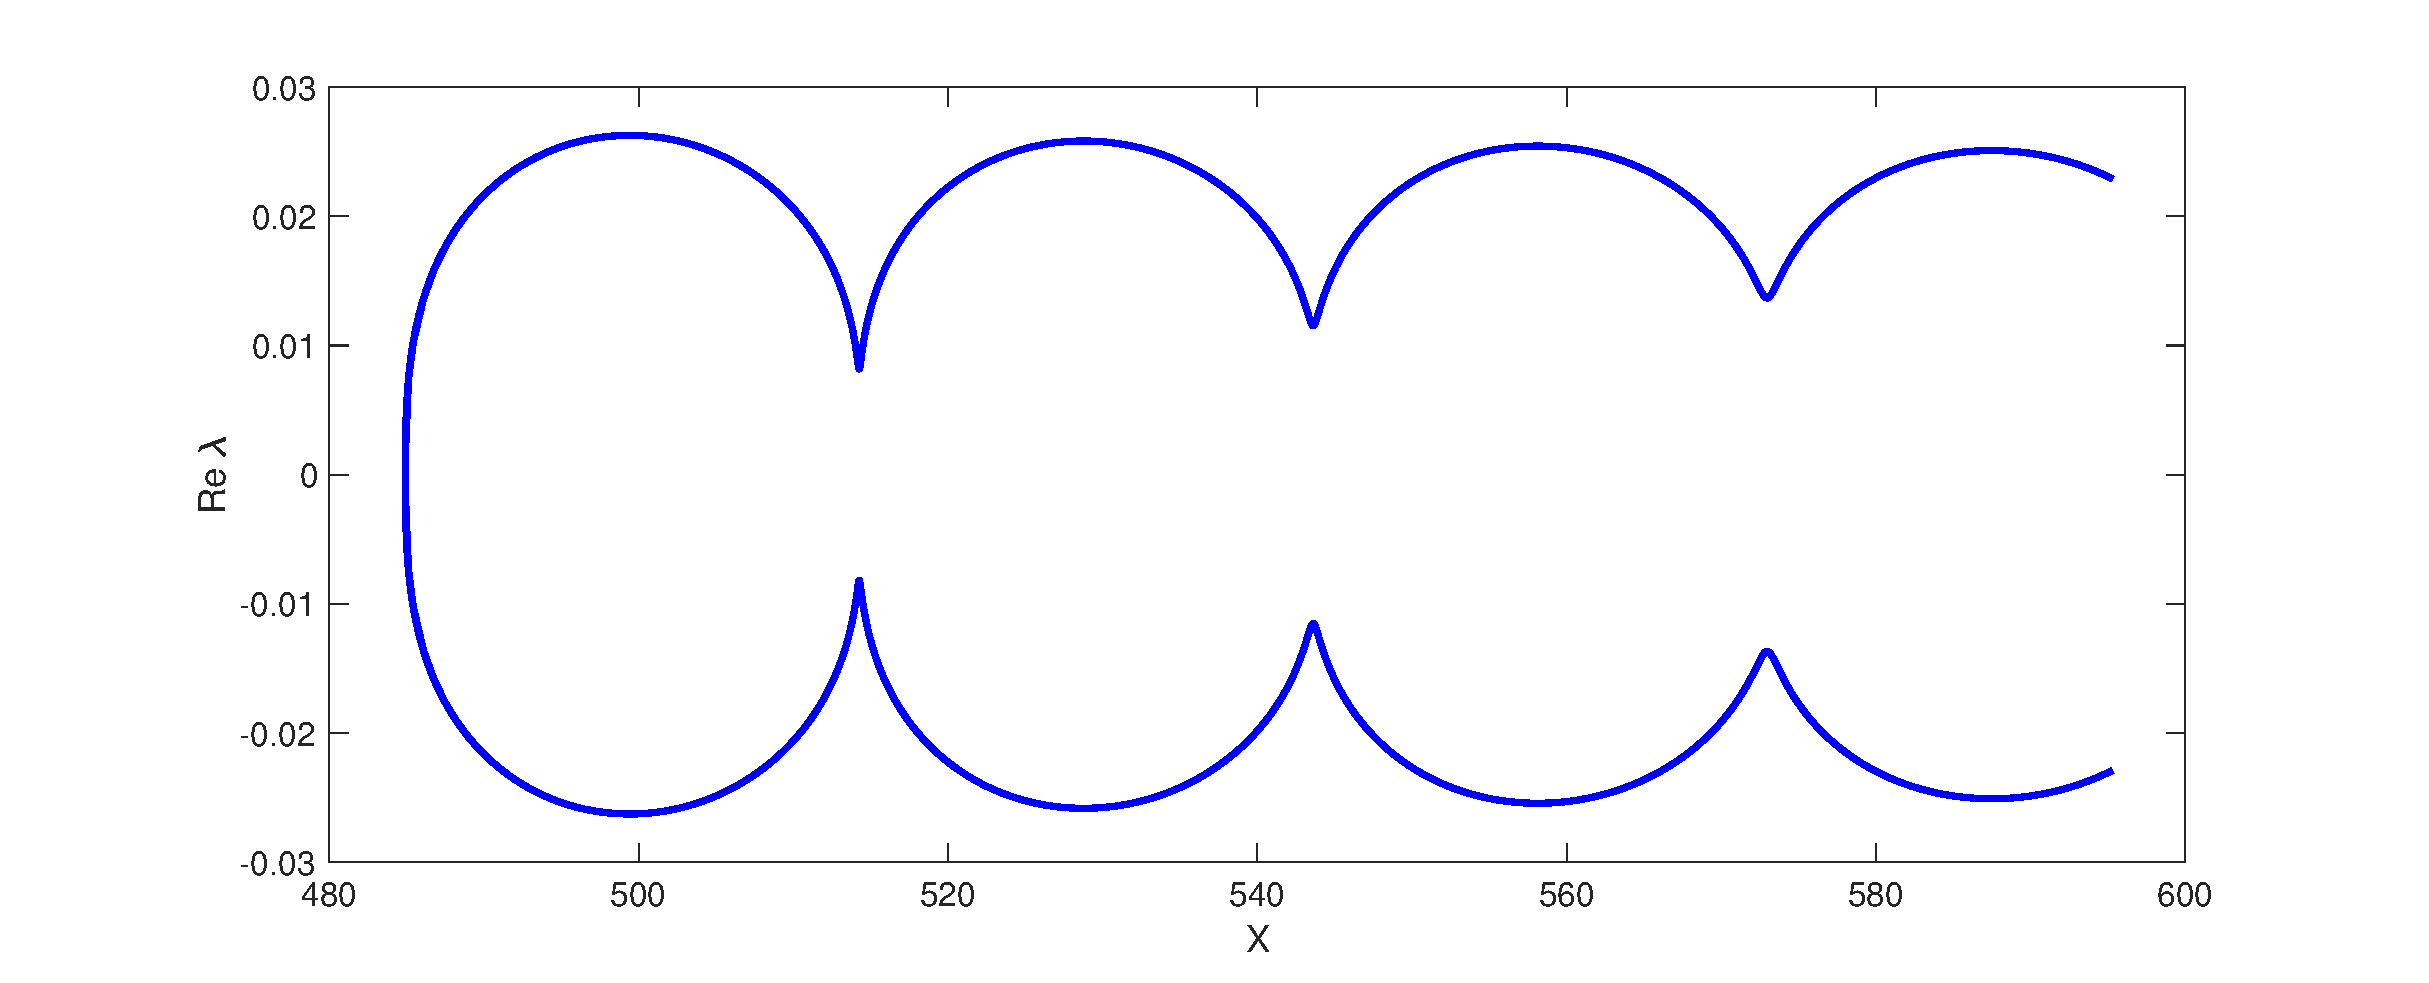
\includegraphics[width=9cm]{images/KreinBubbleCollision.eps}
\end{center}
\caption{Overlapping Krein bubbles as $X$ is increased. Parameter continuation with AUTO, second double pulses with $m_0 = 1$, parameters $p = 6.62$, $c = 10.9561$.}
\label{fig:KreinBubbleCollision}
\end{figure}
\noi After this occurs, we expect that there will always be an eigenvalue with positive real part, thus the periodic double pulses should be unstable for $X > X_c$. As $X$ is further increased, we expect that more than two Krein bubbles will interact and that the eigenvalue behavior will become increasing complicated (this is very difficult to simulate numerically as it involves extremely large domain sizes). In particular, this means that we will cannot generalize the periodic case to obtain the behavior on $\R$ by taking $X\rightarrow \infty$.

\bibliographystyle{amsplain}
\bibliography{kdv5.bib}

\end{document}
